\documentclass[notoc,notitlepage]{tufte-book}
% \nonstopmode % uncomment to enable nonstopmode

\usepackage{classnotetitle}

\title{PMATH351 --- Real Analysis}
\author{Johnson Ng}
\subtitle{Classnotes for Fall 2018}
\credentials{BMath (Hons), Pure Mathematics major, Actuarial Science Minor}
\institution{University of Waterloo}

\setcounter{secnumdepth}{3}
\setcounter{tocdepth}{3}

\renewcommand{\baselinestretch}{1.1}
\usepackage{geometry}
\geometry{letterpaper}
\usepackage[parfill]{parskip}
\usepackage{graphicx}

% Essential Packages
\usepackage{makeidx}
\makeindex
\usepackage{enumitem}
\usepackage[T1]{fontenc}
\usepackage{natbib}
\bibliographystyle{apalike}
\usepackage{ragged2e}
\usepackage{etoolbox}
\usepackage{amssymb}
\usepackage{fontawesome}
\usepackage{amsmath}
\usepackage{mathrsfs}
\usepackage{mathtools}
\usepackage{xparse}
\usepackage{tkz-euclide}
\usetkzobj{all}
\usepackage[utf8]{inputenc}
\usepackage{csquotes}
\usepackage[english]{babel}
\usepackage{marvosym}
\usepackage{pgf,tikz}
\usepackage{pgfplots}
\usepackage{fancyhdr}
\usepackage{array}
\usepackage{faktor}
\usepackage{float}
\usepackage{xcolor}
\usepackage{centernot}
\usepackage{silence}
  \WarningFilter*{latex}{Marginpar on page \thepage\space moved}
\usepackage{tcolorbox}
\tcbuselibrary{skins,breakable}
\usepackage{longtable}
\usepackage[amsmath,hyperref]{ntheorem}
\usepackage{hyperref}
\usepackage[noabbrev,capitalize,nameinlink]{cleveref}

% xcolor (scheme: base16 eighties)
\definecolor{base16-eighties-dark}{HTML}{2D2D2D}
\definecolor{base16-eighties-light}{HTML}{D3D0C8}
\definecolor{base16-eighties-magenta}{HTML}{CD98CD}
\definecolor{base16-eighties-red}{HTML}{F47678}
\definecolor{base16-eighties-yellow}{HTML}{E2B552}
\definecolor{base16-eighties-green}{HTML}{98CD97}
\definecolor{base16-eighties-lightblue}{HTML}{61CCCD}
\definecolor{base16-eighties-blue}{HTML}{6498CE}
\definecolor{base16-eighties-brown}{HTML}{D47B4E}
\definecolor{base16-eighties-gray}{HTML}{747369}

% hyperref Package Settings
\hypersetup{
    bookmarks=true,         % show bookmarks bar?
    unicode=true,          % non-Latin characters in Acrobat’s bookmarks
    pdftoolbar=false,        % show Acrobat’s toolbar?
    pdfmenubar=false,        % show Acrobat’s menu?
    pdffitwindow=true,     % window fit to page when opened
    colorlinks=true,
    allcolors=base16-eighties-magenta,
}

% tikz
\usepgfplotslibrary{polar}
\usepgflibrary{shapes.geometric}
\usetikzlibrary{angles,patterns,calc,decorations.markings}
\tikzset{midarrow/.style 2 args={
        decoration={markings,
            mark= at position #2 with {\arrow{#1}} ,
        },
        postaction={decorate}
    },
    midarrow/.default={latex}{0.5}
}
\def\centerarc[#1](#2)(#3:#4:#5)% Syntax: [draw options] (center) (initial angle:final angle:radius)
    { \draw[#1] ($(#2)+({#5*cos(#3)},{#5*sin(#3)})$) arc (#3:#4:#5); }

% enumitems
\newlist{inlinelist}{enumerate*}{1}
\setlist*[inlinelist,1]{%
  label=(\roman*),
}

% Theorem Style Customization
\setlength\theorempreskipamount{2ex}
\setlength\theorempostskipamount{3ex}

\makeatletter
\let\nobreakitem\item
\let\@nobreakitem\@item
\patchcmd{\nobreakitem}{\@item}{\@nobreakitem}{}{}
\patchcmd{\nobreakitem}{\@item}{\@nobreakitem}{}{}
\patchcmd{\@nobreakitem}{\@itempenalty}{\@M}{}{}
\patchcmd{\@xthm}{\ignorespaces}{\nobreak\ignorespaces}{}{}
\patchcmd{\@ythm}{\ignorespaces}{\nobreak\ignorespaces}{}{}

\renewtheoremstyle{break}%
  {\item{\theorem@headerfont
          ##1\ ##2\theorem@separator}\hskip\labelsep\relax\nobreakitem}%
  {\item{\theorem@headerfont
          ##1\ ##2\ (##3)\theorem@separator}\hskip\labelsep\relax\nobreakitem}
\makeatother

% ntheorem + framed
\makeatletter

% ntheorem Declarations
\theorempreskip{10pt}
\theorempostskip{5pt}
\theoremstyle{break}

\newtheorem*{solution}{\faPencil $\enspace$ Solution}
\newtheorem*{remark}{Remark}
\newtheorem{eg}{Example}[section]
\newtheorem{ex}{Exercise}[section]

    % definition env
\theoremprework{\textcolor{base16-eighties-blue}{\hrule height 2pt}}
\theoremheaderfont{\color{base16-eighties-blue}\normalfont\bfseries}
\theorempostwork{\textcolor{base16-eighties-blue}{\hrule height 2pt}}
\theoremindent10pt
\newtheorem{defn}{\faBook \enspace Definition}

    % definition env no num
\theoremprework{\textcolor{base16-eighties-blue}{\hrule height 2pt}}
\theoremheaderfont{\color{base16-eighties-blue}\normalfont\bfseries}
\theorempostwork{\textcolor{base16-eighties-blue}{\hrule height 2pt}}
\theoremindent10pt
\newtheorem*{defnnonum}{\faBook \enspace Definition}

    % theorem envs
\theoremprework{\textcolor{base16-eighties-magenta}{\hrule height 2pt}}
\theoremheaderfont{\color{base16-eighties-magenta}\normalfont\bfseries}
\theorempostwork{\textcolor{base16-eighties-magenta}{\hrule height 2pt}}
\theoremindent10pt
\newtheorem{thm}{\faCoffee \enspace Theorem}

\theoremprework{\textcolor{base16-eighties-magenta}{\hrule height 2pt}}
\theorempostwork{\textcolor{base16-eighties-magenta}{\hrule height 2pt}}
\theoremindent10pt
\newtheorem{propo}[thm]{\faTint \enspace Proposition}

\theoremprework{\textcolor{base16-eighties-magenta}{\hrule height 2pt}}
\theorempostwork{\textcolor{base16-eighties-magenta}{\hrule height 2pt}}
\theoremindent10pt
\newtheorem{crly}[thm]{\faSpaceShuttle \enspace Corollary}

\theoremprework{\textcolor{base16-eighties-magenta}{\hrule height 2pt}}
\theorempostwork{\textcolor{base16-eighties-magenta}{\hrule height 2pt}}
\theoremindent10pt
\newtheorem{lemma}[thm]{\faTree \enspace Lemma}

\theoremprework{\textcolor{base16-eighties-magenta}{\hrule height 2pt}}
\theorempostwork{\textcolor{base16-eighties-magenta}{\hrule height 2pt}}
\theoremindent10pt
\newtheorem{axiom}[thm]{\faShield \enspace Axiom}

    % theorem envs without counter
\theoremprework{\textcolor{base16-eighties-magenta}{\hrule height 2pt}}
\theoremheaderfont{\color{base16-eighties-magenta}\normalfont\bfseries}
\theorempostwork{\textcolor{base16-eighties-magenta}{\hrule height 2pt}}
\theoremindent10pt
\newtheorem*{thmnonum}{\faCoffee \enspace Theorem}

\theoremprework{\textcolor{base16-eighties-magenta}{\hrule height 2pt}}
\theorempostwork{\textcolor{base16-eighties-magenta}{\hrule height 2pt}}
\theoremindent10pt
\newtheorem*{propononum}{\faTint \enspace Proposition}

\theoremprework{\textcolor{base16-eighties-magenta}{\hrule height 2pt}}
\theorempostwork{\textcolor{base16-eighties-magenta}{\hrule height 2pt}}
\theoremindent10pt
\newtheorem*{crlynonum}{\faSpaceShuttle \enspace Corollary}

\theoremprework{\textcolor{base16-eighties-magenta}{\hrule height 2pt}}
\theorempostwork{\textcolor{base16-eighties-magenta}{\hrule height 2pt}}
\theoremindent10pt
\newtheorem*{lemmanonum}{\faTree \enspace Lemma}

\theoremprework{\textcolor{base16-eighties-magenta}{\hrule height 2pt}}
\theorempostwork{\textcolor{base16-eighties-magenta}{\hrule height 2pt}}
\theoremindent10pt
\newtheorem*{axiomnonum}{\faShield \enspace Axiom}

    % proof env
\theoremprework{\textcolor{base16-eighties-brown}{\hrule height 2pt}}
\theoremheaderfont{\color{base16-eighties-brown}\normalfont\bfseries}
\theorempostwork{\textcolor{base16-eighties-brown}{\hrule height 2pt}}
\newtheorem*{proof}{\faPencil \enspace Proof}

    % note and notation env
\theoremprework{\textcolor{base16-eighties-yellow}{\hrule height 2pt}}
\theoremheaderfont{\color{base16-eighties-yellow}\normalfont\bfseries}
\theorempostwork{\textcolor{base16-eighties-yellow}{\hrule height 2pt}}
\newtheorem*{note}{\faQuoteLeft \enspace Note}

\theoremprework{\textcolor{base16-eighties-yellow}{\hrule height 2pt}}
\theorempostwork{\textcolor{base16-eighties-yellow}{\hrule height 2pt}}
\newtheorem*{notation}{\faPaw \enspace Notation}

    % warning env
\theoremprework{\textcolor{base16-eighties-red}{\hrule height 2pt}}
\theoremheaderfont{\color{base16-eighties-red}\normalfont\bfseries}
\theorempostwork{\textcolor{base16-eighties-red}{\hrule height 2pt}}
\theoremindent10pt
\newtheorem*{warning}{\faBug \enspace Warning}

% more environments
\newtcolorbox{redquote}{
  blanker,enhanced,breakable,standard jigsaw,
  opacityback=0,
  coltext=base16-eighties-light,
  left=5mm,right=5mm,top=2mm,bottom=2mm,
  colframe=base16-eighties-red,
  boxrule=0pt,leftrule=3pt,
  fontupper=\itshape
}
\newtcolorbox{bluequote}{
  blanker,enhanced,breakable,standard jigsaw,
  opacityback=0,
  coltext=base16-eighties-light,
  left=5mm,right=5mm,top=2mm,bottom=2mm,
  colframe=base16-eighties-blue,
  boxrule=0pt,leftrule=3pt,
  fontupper=\itshape
}
\newtcolorbox{greenquote}{
  blanker,enhanced,breakable,standard jigsaw,
  opacityback=0,
  coltext=base16-eighties-light,
  left=5mm,right=5mm,top=2mm,bottom=2mm,
  colframe=base16-eighties-green,
  boxrule=0pt,leftrule=3pt,
  fontupper=\itshape
}
\newtcolorbox{yellowquote}{
  blanker,enhanced,breakable,standard jigsaw,
  opacityback=0,
  coltext=base16-eighties-light,
  left=5mm,right=5mm,top=2mm,bottom=2mm,
  colframe=base16-eighties-yellow,
  boxrule=0pt,leftrule=3pt,
  fontupper=\itshape
}
\newtcolorbox{magentaquote}{
  blanker,enhanced,breakable,standard jigsaw,
  opacityback=0,
  coltext=base16-eighties-light,
  left=5mm,right=5mm,top=2mm,bottom=2mm,
  colframe=base16-eighties-magenta,
  boxrule=0pt,leftrule=3pt,
  fontupper=\itshape
}

% ntheorem listtheorem style
\makeatother
\newlength\widesttheorem
\AtBeginDocument{
  \settowidth{\widesttheorem}{Proposition A.1.1.1\quad}
}

\makeatletter
\def\thm@@thmline@name#1#2#3#4{%
        \@dottedtocline{-2}{0em}{2.3em}%
                   {\makebox[\widesttheorem][l]{#1 \protect\numberline{#2}}#3}%
                   {#4}}
\@ifpackageloaded{hyperref}{
\def\thm@@thmline@name#1#2#3#4#5{%
    \ifx\#5\%
        \@dottedtocline{-2}{0em}{2.3em}%
            {\makebox[\widesttheorem][l]{#1 \protect\numberline{#2}}#3}%
            {#4}
    \else
        \ifHy@linktocpage\relax\relax
            \@dottedtocline{-2}{0em}{2.3em}%
                {\makebox[\widesttheorem][l]{#1 \protect\numberline{#2}}#3}%
                {\hyper@linkstart{link}{#5}{#4}\hyper@linkend}%
        \else
            \@dottedtocline{-2}{0em}{2.3em}%
                {\hyper@linkstart{link}{#5}%
                  {\makebox[\widesttheorem][l]{#1 \protect\numberline{#2}}#3}\hyper@linkend}%
                    {#4}%
        \fi
    \fi}
}

\makeatletter
\def\thm@@thmline@noname#1#2#3#4{%
        \@dottedtocline{-2}{0em}{5em}%
                   {{\protect\numberline{#2}}#3}%
                   {#4}}
\@ifpackageloaded{hyperref}{
\def\thm@@thmline@noname#1#2#3#4#5{%
    \ifx\#5\%
        \@dottedtocline{-2}{0em}{5em}%
            {{\protect\numberline{#2}}#3}%
            {#4}
    \else
        \ifHy@linktocpage\relax\relax
            \@dottedtocline{-2}{0em}{5em}%
                {{\protect\numberline{#2}}#3}%
                {\hyper@linkstart{link}{#5}{#4}\hyper@linkend}%
        \else
            \@dottedtocline{-2}{0em}{5em}%
                {\hyper@linkstart{link}{#5}%
                  {{\protect\numberline{#2}}#3}\hyper@linkend}%
                    {#4}%
        \fi
    \fi}
}

\theoremlisttype{allname}

\AtBeginDocument{\renewcommand\contentsname{Table of Contents}}

% Heading formattings
% chapter format
\titleformat{\chapter}%
  {\huge\rmfamily\itshape\color{base16-eighties-magenta}}% format applied to label+text
  {\llap{\colorbox{base16-eighties-magenta}{\parbox{1.5cm}{\hfill\itshape\huge\textcolor{base16-eighties-dark}{\thechapter}}}}}% label
  {5pt}% horizontal separation between label and title body
  {}% before the title body
  []% after the title body

% section format
\titleformat{\section}%
  {\normalfont\Large\rmfamily\itshape\color{base16-eighties-blue}}% format applied to label+text
  {\llap{\colorbox{base16-eighties-blue}{\parbox{1.5cm}{\hfill\itshape\textcolor{base16-eighties-dark}{\thesection}}}}}% label
  {5pt}% horizontal separation between label and title body
  {}% before the title body
  []% after the title body

% subsection format
\titleformat{\subsection}%
  {\normalfont\large\itshape\color{base16-eighties-green}}% format applied to label+text
  {\llap{\colorbox{base16-eighties-green}{\parbox{1.5cm}{\hfill\textcolor{base16-eighties-dark}{\thesubsection}}}}}% label
  {1em}% horizontal separation between label and title body
  {}% before the title body
  []% after the title body

% Sidenote enhancements
\def\mathmarginnote#1{%
  \tag*{\rlap{\hspace\marginparsep\smash{\parbox[t]{\marginparwidth}{%
  \footnotesize#1}}}}
}

% Custom table columning
\newcolumntype{L}[1]{>{\raggedright\let\newline\\\arraybackslash\hspace{0pt}}m{#1}}
\newcolumntype{C}[1]{>{\centering\let\newline\\\arraybackslash\hspace{0pt}}m{#1}}
\newcolumntype{R}[1]{>{\raggedleft\let\newline\\\arraybackslash\hspace{0pt}}m{#1}}

% Custom math operator
% \DeclareMathOperator{\rem}{rem}
\DeclareMathOperator*{\argmax}{arg\,max}
\DeclareMathOperator*{\argmin}{arg\,min}
\DeclareMathOperator{\re}{Re}
\DeclareMathOperator{\im}{Im}
\DeclareMathOperator{\caparg}{Arg}
\DeclareMathOperator{\Ind}{Ind}
\DeclareMathOperator{\Res}{Res}

% Graph styles
\pgfplotsset{compat=1.15}
\usepgfplotslibrary{fillbetween}
\pgfplotsset{four quads/.append style={axis x line=middle, axis y line=
middle, xlabel={$x$}, ylabel={$y$}, axis equal }}
\pgfplotsset{four quad complex/.append style={axis x line=middle, axis y line=
middle, xlabel={$\re$}, ylabel={$\im$}, axis equal }}

% Shortcuts
\newcommand{\floor}[1]{\lfloor #1 \rfloor}      % simplifying the writing of a floor function
\newcommand{\ceiling}[1]{\lceil #1 \rceil}      % simplifying the writing of a ceiling function
\newcommand{\dotp}{\, \cdotp}			        % dot product to distinguish from \cdot
\newcommand{\qed}{\hfill\ensuremath{\square}}   % Q.E.D sign
\newcommand{\abs}[1]{\left|#1\right|}						% absolute value
\newcommand{\lra}[1]{\langle \; #1 \; \rangle}
\newcommand{\at}[2]{\Big|_{#1}^{#2}}
\newcommand{\Arg}[1]{\caparg #1}
\renewcommand{\bar}[1]{\mkern 1.5mu \overline{\mkern -1.5mu #1 \mkern -1.5mu} \mkern 1.5mu}
\newcommand{\quotient}[2]{\faktor{#1}{#2}}
\newcommand{\cyclic}[1]{\left\langle #1 \right\rangle}
	% highlighting shortcuts
\newcommand{\hlimpo}[1]{\textcolor{base16-eighties-red}{\textbf{#1}}}
\newcommand{\hlwarn}[1]{\textcolor{base16-eighties-yellow}{\textbf{#1}}}
\newcommand{\hldefn}[1]{\textcolor{base16-eighties-blue}{\index{#1}\textbf{#1}}}
\newcommand{\hlnotea}[1]{\textcolor{base16-eighties-green}{\textbf{#1}}}
\newcommand{\hlnoteb}[1]{\textcolor{base16-eighties-lightblue}{\textbf{#1}}}
\newcommand{\hlnotec}[1]{\textcolor{base16-eighties-brown}{\textbf{#1}}}
\newcommand{\WTP}{\textcolor{base16-eighties-brown}{WTP} }
\newcommand{\WTS}{\textcolor{base16-eighties-brown}{WTS} }
\newcommand{\ind}[2]{\Ind_{#2}\left( #1 \right)}
\newcommand{\notimply}{\centernot\implies}
\newcommand{\res}[2]{\underset{#2}{\Res} #1 }
\newcommand{\tworow}[3]{\begin{tabular}{@{}#1@{}} #2 \\ #3 \end{tabular}}
\renewcommand{\epsilon}{\varepsilon}
\newcommand{\lrarrow}{\leftrightarrow}
\newcommand{\larrow}{\leftarrow}
\newcommand{\rarrow}{\rightarrow}
\renewcommand{\atop}[2]{\genfrac{}{}{0pt}{}{#1}{#2}}
\newcommand*\dif{\mathop{}\!d}

  % inspiration from: https://tex.stackexchange.com/questions/8720/overbrace-underbrace-but-with-an-arrow-instead#37758
\newcommand{\overarrow}[2]{
  \overset{\makebox[0pt]{\begin{tabular}{@{}c@{}}#2\\[0pt]\ensuremath{\uparrow}\end{tabular}}}{#1}
}
\newcommand{\underarrow}[2]{
  \underset{\makebox[0pt]{\begin{tabular}{@{}c@{}}\downarrow\\[0pt]\ensuremath{#2}\end{tabular}}}{#1}
}

% Document header formatting
\renewcommand{\chaptermark}[1]{\markboth{#1}{}}
\renewcommand{\sectionmark}[1]{\markright{#1}}
\makeatletter
\pagestyle{fancy}
\fancyhead{}
\fancyhead[RO]{\textsl{\@title} \enspace \thepage}
\fancyhead[LE]{\thepage \enspace \textsl{\leftmark \enspace - \enspace \rightmark}}
\makeatother

% Comment the two lines below if you want to print the document
\pagecolor{base16-eighties-dark}
\color{base16-eighties-light}


\DeclareMathOperator{\lub}{lub }
\DeclareMathOperator{\glb}{glb }
\DeclareMathOperator{\Range}{Range }
\DeclareMathOperator{\Domain}{Domain }
\DeclareMathOperator{\bdy}{bdy }
\DeclareMathOperator{\Lim}{Lim }
\DeclareMathOperator{\diam}{diam }

\newcommand{\norm}[1]{\left\| #1 \right\|}

\begin{document}
\hypersetup{pageanchor=false}
\maketitle
\hypersetup{pageanchor=true}
\begin{fullwidth}
\tableofcontents
\end{fullwidth}

\chapter*{\faBook\ \enspace\ List of Definitions}
\addcontentsline{toc}{chapter}{List of Definitions}
\theoremlisttype{all}
\begin{fullwidth}
\listtheorems{defn}
\end{fullwidth}

\chapter*{\faCoffee\ \enspace\ List of Theorems}
\addcontentsline{toc}{chapter}{List of Theorems}
\theoremlisttype{allname}
\begin{fullwidth}
\listtheorems{axiom,lemma,thm,crly,propo}
\end{fullwidth}

\nocite{bforres2018}

\chapter{Lecture 1 Sep 06th}%
\label{chp:lecture_1_sep_06th}
% chapter lecture_1_sep_06th

\section{Course Logistics}%
\label{sec:course_logistics}
% section course_logistics

No content is covered in today's lecture so this chapter will cover some of the important logistical highlights that were mentioned in class.

\begin{itemize}
  \item Assignments are designed to help students understand the content.
  \item Due to shortage of manpower, not all assignment questions will be graded; however, students are encouraged to attempt all of the questions.
  \item To further motivate students to work on ungraded questions, the midterm and final exam will likely recycle some of the assignment questions.
  \item There are no required text, but the professor has prepared course notes for reading. The course note are self-contained.
  \item The approach of the class will be more interactive than most math courses.
  \item Due to the size of the class, students are encouraged to utilize Waterloo Learn for questions, so that similar questions by multiple students can be addressed at the same time.
\end{itemize}

% section course_logistics (end)

\section{Preview into the Introduction}%
\label{sec:preview_into_the_introduction}
% section preview_into_the_introduction

How do we compare the size of two sets?

\begin{itemize}
  \item If the sets are finite, this is a relatively easy task.
  \item If the sets are infinite, we will have to rely on functions.
    \begin{itemize}
      \item Injective functions tell us that the \hlnoteb{domain is of size that is lesser than or equal to the codomain}.
      \item Surjective functions tell us that the \hlnoteb{codomain is of size that is lesser than or equal to the domain}.
      \item So does a bijective function tell us that the domain and codomain have the same size? Yes, although this is not as intuitive as it looks, as it relies on \hlnotea{Cantor-Schr\"oder-Bernstein Theorem}.
    \end{itemize}
\end{itemize}

Now, given two arbitrary sets, are we guaranteed to always be able to compare their sizes? It is tempting to immediately say yes, but to do that, one would have to agree on the \hlnotea{Axiom of Choice}. Fortunately, within the realm of this course, the Axiom of Choice is taken for granted.

% section preview_into_the_introduction (end)

% chapter lecture_1_sep_06th (end)

\chapter{Lecture 2 Sep 10th}%
\label{chp:lecture_2_sep_10th}
% chapter lecture_2_sep_10th

\section{Basic Set Theory}%
\label{sec:basic_set_theory}
% section basic_set_theory

We shall use the following notations for some of the common set of numbers that we are already familiar with:
\begin{itemize}
  \item $\mathbb{N}$ denotes the set of natural numbers $\{1, 2, 3, \ldots\}$;
  \item $\mathbb{Z}$ denotes the set of integers $\{\ldots, -2, -1, 0, 1, 2, \ldots\}$;
  \item $\mathbb{Q}$ denotes the set of rational numbers $\left\{ \frac{a}{b} \mid a \in \mathbb{Z}, b \in \mathbb{N} \right\}$; and
  \item $\mathbb{R}$ denotes the set of real numbers.
\end{itemize}

We shall start with having certain basic properties of $\mathbb{N}$, $\mathbb{Z}$, and $\mathbb{Q}$.

\newthought{We will use} the notation $A \subset B$ and $A \subseteq B$ interchangably to mean that $A$ is a subset of $B$ with the possibility that $A = B$. When we wish to explicitly emphasize this possibility, we shall use $A \subseteq B$. When we wish to explicitly state that $A$ is a \hlnotea{proper subset} of $B$, we will either specify that $A \neq B$ or simply $A \subsetneq B$.

\begin{defn}[Universal Set]\index{Universal Set}\label{defn:universal_set}\marginnote{This is a hand-wavy definition, but it is not in the interest of this course to further explore on this topic.}
  A universal set, which we shall generally give the label $X$, is a set that contains all the mathematical objects that we are interested in.
\end{defn}

With a universal set in place, we can have the following definitions:

\begin{defn}[Union]\index{Union}\label{defn:union}
  Let $X$ be a set. If ${\{A_\alpha\}}_{\alpha \in I}$ such that $A_{\alpha} \subset X$, then the \hlnoteb{union} for all $A_{\alpha}$ is defined as
  \begin{equation*}
    \bigcup_{\alpha \in I} A_{\alpha} := \{ x \in X \mid \exists \alpha \in I, x \in A_{\alpha} \}.
  \end{equation*}
\end{defn}

\begin{defn}[Intersection]\index{Intersection}\label{defn:intersection}
  Let $X$ be a set. If ${\{A_\alpha\}}_{\alpha \in I}$ such that $A_\alpha \subset X$, then the \hlnoteb{intersection} for all $A_\alpha$ is defined as
  \begin{equation*}
    \bigcap_{\alpha \in I} A_\alpha := \{ x \in X \mid \forall \alpha \in I, x \in A_\alpha \}.
  \end{equation*}
\end{defn}

\begin{defn}[Set Difference]\index{Set Difference}\label{defn:set_difference}
  Let $X$ be a set and $A, B \subseteq X$. The \hlnoteb{set difference} of $A$ from $B$ is defined as
  \begin{equation*}
    A \setminus B := \{ x \in X \mid x \in A, x \notin B \}.
  \end{equation*}
\end{defn}

On a similar notion:

\begin{defn}[Symmetric Difference]\index{Symmetric Difference}\label{defn:symmetric_difference}
Let $X$ be a set and $A, B \subseteq X$. The \hlnoteb{symmetric difference} of $A$ and $B$ is defined as\marginnote{In words, for an element in the symmetric difference of two sets, the element is either in $A$ or $B$ but not both. We can also think of the symmetric difference as
\begin{equation*}
  ( A \cup B ) \setminus (A \cap B)
\end{equation*}
or
\begin{equation*}
  ( A \setminus B ) \cup (B \setminus A).
\end{equation*}
}
  \begin{equation*}
    A \Delta B := \{ x \in X \mid ( x \in A \land x \notin B ) \lor ( x \notin A \land x \in B ) \}.
  \end{equation*}
\end{defn}

We can also talk about the non-members of a set:

\begin{defn}[Set Complement]\index{Set Complement}\label{defn:set_complement}
  Let $X$ be a set and $A \subset X$. The set of all non-members of $A$ is called the \hlnoteb{complement} of $A$, which we denote as
  \begin{equation*}
    A^c := \{ x \in X \mid x \notin A \}.
  \end{equation*}
\end{defn}

\begin{note}
  Note that
  \begin{equation*}
    {\left( A^c \right)}^c = \{ x \in X \mid x \notin A^c \} = \{ x \in X \mid x \in A \} = A.
  \end{equation*}
\end{note}

Now taking a step away from that, we define the following:

\begin{defn}[Empty Set]\index{Empty Set}\label{defn:empty_set}
  An \hlnoteb{empty set}, denoted by $\emptyset$, is a set that contains nothing.
\end{defn}

\begin{note}
  The empty set is set to be a subset of all sets.
\end{note}

\begin{defn}[Power Set]\index{Power Set}\label{defn:power_set}
  Let $X$ be a set. The power set of $X$ is the set that contains all subsets of $X$, i.e.
  \begin{equation*}
    \mathcal{P}(X) := \{ A \mid A \subset X \}.
  \end{equation*}
\end{defn}

\begin{note}
  A power set is always non-empty, since $\emptyset \in \mathcal{P}(\emptyset)$, and since $\emptyset \subset X$ for any set $X$, we have $\emptyset \in \mathcal{P}(X)$.
\end{note}

\begin{eg}
  Let $X = \{1, 2, \ldots, n\}$. There are several ways we can show that the size of $\mathcal{P}(X)$ is $2^n$. One of the methods is by using a characteristic function that maps from $A$ to $\{0, 1\}$, defined by
  \begin{gather*}
    X_A: A \to \{0, 1\} \\
    X_A(x) = \begin{cases}
      1 & x \in A \\
      0 & x \notin A
    \end{cases}.
  \end{gather*}
  Using this function, each element in $X$ have 2 states: one being in the subset, and the other being not in the subset, which are represented by $1$ and $0$ respectively. It is then clear that there are $2^n$ of such configurations.
\end{eg}

\begin{thm}[De Morgan's Laws]\index{De Morgan's Laws}\label{thm:de_morgan_s_laws}
  Let $X$ be a set. Given ${\{A_\alpha\}}_{\alpha \in I} \subset \mathcal{P}(X)$, we have
  \begin{enumerate}
    \item ${\left( \bigcup\limits_{\alpha \in I} A_\alpha \right)}^c = \bigcap\limits_{\alpha \in I} A_\alpha^c$; and
    \item ${\left( \bigcap\limits_{\alpha \in I} A_\alpha \right)}^c = \bigcup\limits_{\alpha \in I} A_\alpha^c$.
  \end{enumerate}
\end{thm}

\begin{proof}
  \begin{enumerate}
    \item Note that
      \begin{align*}
        x \in {\left( \bigcup_{\alpha \in I} A_\alpha \right)}^c &\iff \nexists \alpha \in I \enspace x \in A_\alpha \\
        &\iff \forall \alpha \in I \enspace x \notin A_\alpha \\
        &\iff \forall \alpha \in I \enspace x \in A_\alpha^c \text{ by set complementation } \\
        &\iff x \in \bigcap_{\alpha \in I} A_\alpha^c.
      \end{align*}

    \item Observe that, by part 1,
      \begin{align*}
        {\left( \bigcap_{\alpha \in I} A_\alpha \right)}^c = {\left( {\left( \bigcup_{\alpha \in I} A_{\alpha}^c \right)}^c \right)}^c = \bigcup_{\alpha \in I} A_\alpha^c.
      \end{align*}
  \end{enumerate}\qed\
\end{proof}

\begin{eg}
  Suppose $I = \emptyset$. Then what is $\bigcup\limits_{\alpha \in \emptyset} A_\alpha$? It is sensible to think that all we are left with is simply a union of empty sets, and so
  \begin{equation}\label{eq:union_of_empty_sets}
    \bigcup_{\alpha \in \emptyset} A_\alpha = \emptyset.
  \end{equation}
  And what about $\bigcap\limits_{\alpha \in \emptyset} A_\alpha$? By \cref{thm:de_morgan_s_laws}, it is quite clear from \cref{eq:union_of_empty_sets} that
  \begin{equation*}
    \bigcap_{\alpha \in \emptyset} A_\alpha = X.
  \end{equation*}
\end{eg}

% section basic_set_theory (end)

\section{Products of Sets}%
\label{sec:products_of_sets}
% section products_of_sets

\begin{defn}[Product of Sets]\index{Product of Sets}\label{defn:product_of_sets}
  Given $2$ sets $X$ and $Y$, the \hlnoteb{product} of $X$ and $Y$ is given by
  \begin{equation*}
    X \times Y := \{ (x, y) \mid x \in X , y \in Y \}.
  \end{equation*}
  We often refer to elements of $X \times Y$ as \hldefn{tuples}.
\end{defn}

\begin{note}
  Now if
  \begin{align*}
    X &= \{ x_1, x_2, \ldots, x_n \}, \\
    Y &= \{ y_1, y_2, \ldots, y_m \},
  \end{align*}
  then
  \begin{equation*}
    X \times Y = \{ (x_i, y_j) \mid i = 1, 2, \ldots, n, \; j = 1, 2, \ldots, m \}
  \end{equation*}
  and so the size of $X \times Y$ is $mn$.
\end{note}

Consequently, we can think of tuples as two elements being in some ``relation''.

\begin{defn}[Relation]\index{Relation}\label{defn:relation}
  A \hlnoteb{relation} on sets $X$ and $Y$ is a subset $R$ of the product $X \times Y$. We write
  \begin{equation*}
    xRy \enspace \text{ if } (x, y) \in R \subset X \times Y.
  \end{equation*}
  We call
  \begin{itemize}
    \item $\{ x \in X \mid \exists y \in Y, (x, y) \in R \}$ as the \hldefn{domain} of $R$; and 
    \item $\{ y \in Y \mid \exists x \in X, (x, y) \in R \}$ as the \hldefn{range} of $R$.
  \end{itemize}
\end{defn}

In relation to that, functions are, essentially, relations.

\begin{defn}[Function]\index{Function}\label{defn:function}
  A \hlnoteb{function} from $X$ to $Y$ is a relation $R$ such that
  \begin{equation*}
    \forall x \in X \; \exists! y \in Y \; (x, y) \in R.
  \end{equation*}
\end{defn}

\newthought{Suppose} $X_1, X_2, \ldots, X_n$ are non-empty\sidenote{We are typically only interested in non-empty sets, since empty sets usually lead us to vacuous truths, which are not interesting.} sets. We can define
\begin{equation*}
  X_1 \times X_2 \times \hdots \times X_n = \prod_{i=1}^{n} X_i := \{ (x_1, x_2, \ldots, x_n) \mid x_i \in X_i \}.
\end{equation*}
Now if $X_i = X_j = X$ for all $i, j = 1, 2, \ldots, n$, we write
\begin{equation*}
  \prod_{i=1}^{n} X_i = \prod_{i=1}^{n} X = X^n.
\end{equation*}

\newthought{And now comes the problem}: given a collection ${\{X_\alpha\}}_{\alpha \in I}$ of non-empty sets\sidenote{i.e.\ we now talk about arbitrary $\alpha \in I$.}, what do we mean by
\begin{equation*}
  \prod_{\alpha \in I} X_\alpha?
\end{equation*}

To motivate for what comes next, consider
\begin{equation*}
  \prod_{i=1}^{n} X_i = X_1 \times \hdots \times X_n = \{ (x_1, \ldots, x_n) \mid x_i \in X_i \}.
\end{equation*}
Choose $(x_1, \ldots, x_n) \in \prod\limits_{i=1}^{n} X_i$. This induces a function
\begin{equation*}
  f_{(x_1, \ldots, x_n)} : \{1, \ldots, n\} \to \bigcup_{i=1}^{n} X_i
\end{equation*}
with
\begin{align*}
  f(1) &= x_1 \in X_1 \\
  f(2) &= x_2 \in X_2 \\
       &\vdots \\
  f(n) &= x_n \in X_n
\end{align*}

Now assume for a more general $f$ such that
\begin{equation*}
  f: \{1, \ldots, n\} \to \bigcup_{i=1}^{n} X_i
\end{equation*}
is defined by
\begin{equation*}
  f(i) \in X_i.
\end{equation*}
Then, we have
\begin{equation*}
  ( f(1), f(2), \ldots, f(n) ) \in \prod_{i=1}^{n} X_i,
\end{equation*}
which leads us to the following notion:

\begin{defn}[Choice Function]\index{Choice Function}\label{defn:choice_function}
  Given a collection ${\{X_\alpha\}}_{\alpha \in I}$ of non-empty sets, let
  \begin{equation*}
    \prod_{\alpha \in I} X_\alpha = \left\{ f: I \to \bigcup_{\alpha \in I} X_\alpha \right\}
  \end{equation*}
  such that $f(\alpha) \in X_\alpha$. Such an $f$ is called a \hlnoteb{choice function}.
\end{defn}

And so we may ask a similar question as before: if each $X_\alpha$ is non-empty, is $\prod\limits_{\alpha \in I} X_\alpha$ non-empty? Turns out this is not as easy to show. In fact, it is essentially impossible to show, because this is exactly the \hlnotea{Axiom of Choice}.

% section products_of_sets (end)

% chapter lecture_2_sep_10th (end)

\chapter{Lecture 3 Sep 12th}%
\label{chp:lecture_3_sep_12th}
% chapter lecture_3_sep_12th

\section{Axiom of Choice}%
\label{sec:axiom_of_choice}
% section axiom_of_choice

\newthought{Recall} our final question of last lecture: If ${\{ X_\alpha \}}_{\alpha \in I}$ is a non-empty collection of non-empty sets, is
\begin{equation*}
  \prod_{\alpha \in I} X_\alpha \neq \emptyset \enspace?
\end{equation*}

Turns out this is widely known (in the world of mathematics) as the \hlnotea{Axiom of Choice}.

\begin{axiom}[Zermelo's Axiom of Choice]\index{Zermelo's Axiom of Choice}\index{Axiom of Choice}\label{axiom:zermelo_s_axiom_of_choice}
  If ${\{ X_\alpha \}}_{\alpha \in I}$ is a non-empty collection of non-empty sets, then
  \begin{equation*}
    \prod_{\alpha \in I} X_\alpha \neq \emptyset.
  \end{equation*}
\end{axiom}

An equivalent statement of the above axiom is:

\begin{axiom}[Zermelo's Axiom of Choice v2]\index{Zermelo's Axiom of Choice}\index{Axiom of Choice}\label{axiom:zermelo_s_axiom_of_choice_v2}
  $X \neq \emptyset \implies$
  \begin{equation*}
    \exists f : \mathcal{P}(X) \setminus \{ \emptyset \} \to X \; \forall A \in \mathcal{P}(X) \setminus \{ \emptyset \} \; f(A) \in A
  \end{equation*}
  where $f$ is the \hyperref[defn:choice_function]{choice function}.
\end{axiom}

\begin{ex}
  Prove that \cref{axiom:zermelo_s_axiom_of_choice} and \cref{axiom:zermelo_s_axiom_of_choice_v2} are equivalent.
\end{ex}

\begin{proof}
  \textbf{From \cref{axiom:zermelo_s_axiom_of_choice} to \cref{axiom:zermelo_s_axiom_of_choice_v2}}:

  Since $X \neq \emptyset$, we have that $\mathcal{P}(X) \setminus \{ \emptyset \}$ is a non-empty collection of non-empty sets. Therefore,
  \begin{equation*}
    \prod_{A \in \mathcal{P}(X) \setminus \{ \emptyset \} } A \neq \emptyset.
  \end{equation*}
  So we know that
  \begin{equation*}
    \exists {( x_A )}_{A \in \mathcal{P}(X) \setminus \{ \emptyset \} } \in \prod_{A \in \mathcal{P}(X) \setminus \{ \emptyset \} } A.
  \end{equation*}
  We then simply need to choose the choice function $f : \mathcal{P}(X) \setminus \{ \emptyset \} \to X$ such that
  \begin{equation*}
    f(A) = x_A \in A.
  \end{equation*}

  \noindent\textbf{From \cref{axiom:zermelo_s_axiom_of_choice_v2} to \cref{axiom:zermelo_s_axiom_of_choice}}: 

  Let $X_\alpha \in \mathcal{P}(X)$ for $\alpha \in I$, where $I$ is some index set. We know that not all $X_\alpha = \emptyset$ since $X \neq \emptyset$. Choose $J \subseteq I$ such that ${\{ X_\alpha \}}_{\alpha \in J}$ is a non-empty collection of non-empty sets. Let $f: \mathcal{P}(X) \setminus \{ \emptyset \}$ be any choice function. By \cref{axiom:zermelo_s_axiom_of_choice_v2}, 
  \begin{equation*}
    \forall X_\alpha \in \mathcal{P}(X) \setminus \{ \emptyset \} \quad f(X_\alpha) \in X_\alpha.
  \end{equation*}
  Therefore,
  \begin{equation*}
    {( f(X_\alpha) )}_{\alpha \in J} \in \prod_{\alpha \in J} X_\alpha.
  \end{equation*}\qed\
\end{proof}

% section axiom_of_choice (end)

\section{Relations}%
\label{sec:relations}
% section relations

Now, it is in our interest to start talking about comparisons or relations between the mathematical objects that we have defined.

\begin{defn}[Relations]\index{Relations}\label{defn:relations}
  A relation $R$ on a set $X$ is \sidenote{We can look at this definition as $R \subseteq X \times X$. Under such a definition, we would have
  \begin{itemize}
    \item (\textbf{Reflexive}) $\forall x \in X \enspace (x, x) \in R$;
    \item (\textbf{Symmetric}) $\forall x, y \in X \enspace (x, y) \in R \iff (y, x) \in R$;
    \item (\textbf{Anti-symmetric}) $\forall x, y \in X \enspace (x, y), (y, x) \in R \implies x = y$;
    \item (\textbf{Transitive}) $\forall x, y, z \in X \enspace (x, y), (y, z) \in R \implies (x, z) \in R$.
  \end{itemize}}
  \begin{itemize}
    \item (\hldefn{Reflexive}) $\forall x \in X \enspace xRx$;
    \item (\hldefn{Symmetric}) $\forall x, y \in X \enspace xRy \iff yRx$;
    \item (\hldefn{Anti-symmetric}) $\forall x, y \in X \enspace xRy \land yRx \implies x = y$;
    \item (\hldefn{Transitive}) $\forall x, y , z \in X \enspace xRy \land yRz \implies xRz$.
  \end{itemize}
\end{defn}

\begin{eg}
  Let $X = \mathbb{R}$, and let $xRy \iff x \leq y$, where $\leq$ is the notion of ``less than or equal to'', which we shall assume that it has the meaning that we know. Observe that $\leq$ is:
  \begin{itemize}
    \item reflexive: $\forall x \in \mathbb{R} \enspace x \leq x$ is true;
    \item anti-symmetric: $\forall x, y \in \mathbb{R} \enspace x \leq y \land y \leq x \implies x = y$; and
    \item transitive: $\forall x, y , z \in \mathbb{R} \enspace x \leq y \land y \leq z \implies x \leq z$.
  \end{itemize}
\end{eg}

\begin{eg}
  Let $Y \neq \emptyset, \, X = \mathcal{P}(Y)$, with $ARB \iff A \subseteq B$. Observe that $\subseteq$ is:
  \begin{itemize}
    \item reflexive: $\forall A \in \mathcal{P}(Y) \enspace ARA \iff A \subseteq A$ is true;
    \item anti-symmetric: $\forall A, B \in \mathcal{P}(Y) \enspace ARB \land BRA \iff A \subseteq B \land B \subseteq A \implies A = B$;
    \item transitive: $\forall A, B, C \in \mathcal{P}(Y) \enspace ARB \land BRC \iff A \subseteq B \land B \subseteq C \implies A \subseteq C$.
  \end{itemize}
\end{eg}

\begin{eg}
  Let $Y \neq \emptyset, \, X = \mathcal{P}(Y)$, with $ARB \iff A \supseteq B$. Observe that $\supseteq$ is:
  \begin{itemize}
    \item reflexive: $\forall A \in \mathcal{P}(Y) \enspace ARA \iff A \subseteq A$;
    \item anti-symmetric: $\forall A, B \in \mathcal{P}(Y) \enspace ARB \land BRA \iff A \supseteq B \land B \supseteq A \implies A = B$;
    \item transitive: $\forall A, B, C \in \mathcal{P}(Y) \enspace ARB \land BRC \iff A \supseteq B \land B \supseteq C \implies A \supseteq C$.
  \end{itemize}
\end{eg}

All the above examples are also known as \textit{partially ordered sets}.

\begin{defn}[Partially Ordered Sets]\index{Partially Ordered Sets}\index{Poset}\label{defn:partially_ordered_sets}
The set $X$ with the relation $R$ on $X$ is called a \hlnoteb{partially ordered set} (or a \hlnoteb{poset}) if $R$ is\marginnote{The ``partial'' in `partially ordered'' indicates that not every pair of elements need to be comparable, i.e.\ there may be pairs for which neither precedes the other (anti-symmetry).}
  \begin{itemize}
    \item reflexive;
    \item anti-symmetric; and
    \item transitive.
  \end{itemize}
  We denote a poset by $(X, R)$.
\end{defn}

\begin{note}
  If $(X, R)$ is a poset, then if $A \subseteq X$, and $R_1 = R \restriction_{A \times A}$, then $(A, R_1)$ is also a poset.
\end{note}

\begin{eg}\label{eg:number_of_posets}
  How many possible relations can we define on these sets to make them into posets?
  \begin{enumerate}
    \item $X = \emptyset$
      \begin{solution}
        We have that $R = \emptyset \times \emptyset$, and so the only relation we have is an empty relation. Then it is vacuously true that $(X, R)$ a poset.
      \end{solution}
    \item $X = \{ x \}$
      \begin{solution}
        We have that $R = X \times X = \{ ( x, x ) \}$. It it clear that $(X, R)$ is a poset.
      \end{solution}
    \item $X = \{ x, y \}$
      \begin{solution}
        There are 3 possible relations:\marginnote{
          3 possibilities represented as graphs (known as \href{https://en.wikipedia.org/wiki/Hasse_diagram}{Hasse diagram}\index{Hasse diagram}), separated by lines:

        \begin{tikzpicture}
          \node[circle,fill,inner sep=1pt,label={right:{$x$}}] at (1, 3) {};
          \node[circle,fill,inner sep=1pt,label={right:{$y$}}] at (3, 3) {};

          \draw[-] (0,2.5) -- (4,2.5);

          \node[circle,fill,inner sep=1pt,label={right:{$x$}}] at (1, 2) {};
          \draw[-] (1,2) -- (1,1);
          \node[circle,fill,inner sep=1pt,label={right:{$y$}}] at (1, 1) {};

          \draw[-] (2,2.5) -- (2,0.5);

          \node[circle,fill,inner sep=1pt,label={0:{$y$}}] at (3, 2) {};
          \draw[-] (3,2) -- (3,1);
          \node[circle,fill,inner sep=1pt,label={right:{$x$}}] at (3, 1) {};
        \end{tikzpicture}
        }
        \begin{itemize}
          \item a relation where $xRx$ and $yRy$;
          \item a relation where $xRy$; or
          \item a relation where $yRx$.
        \end{itemize}
      \end{solution}
    \item $X = \{ x, y, z \}$
      \begin{solution}
        The following are all the possibilities represented by graphs, where the underlined numbers represent the number of ways we can rearrange the elements for unique relations:

        \begin{center}
          \begin{tikzpicture}
            \node[circle,fill,inner sep=1pt,label={right:{$x$}}] at (1, 3) {};
            \node[circle,fill,inner sep=1pt,label={right:{$y$}}] at (2, 3) {};
            \node[circle,fill,inner sep=1pt,label={right:{$z$}}] at (3, 3) {};
            \node at (-2,3) {\underline{1}};

            \node[circle,fill,inner sep=1pt,label={right:{$x$}}] at (-1, 2) {};
            \node[circle,fill,inner sep=1pt,label={right:{$y$}}] at (1, 2) {};
            \node[circle,fill,inner sep=1pt,label={right:{$z$}}] at (0, 1) {};
            \draw[-] (-1,2) -- (0,1);
            \draw[-] (1,2) -- (0,1);
            \node at (-2,1.5) {\underline{3}};

            \node[circle,fill,inner sep=1pt,label={right:{$x$}}] at (3, 1) {};
            \node[circle,fill,inner sep=1pt,label={right:{$y$}}] at (5, 1) {};
            \node[circle,fill,inner sep=1pt,label={right:{$z$}}] at (4, 2) {};
            \draw[-] (4,2) -- (3,1);
            \draw[-] (4,2) -- (5,1);
            \node at (6,1.5) {\underline{3}};

            \node[circle,fill,inner sep=1pt,label={right:{$x$}}] at (-1, 0) {};
            \node[circle,fill,inner sep=1pt,label={right:{$y$}}] at (1, 0) {};
            \node[circle,fill,inner sep=1pt,label={right:{$z$}}] at (1, -1) {};
            \draw[-] (1,0) -- (1,-1);
            \node at (-2,-0.5) {\underline{6}};

            \node[circle,fill,inner sep=1pt,label={right:{$x$}}] at (4, 0) {};
            \node[circle,fill,inner sep=1pt,label={right:{$y$}}] at (4, -0.5) {};
            \node[circle,fill,inner sep=1pt,label={right:{$z$}}] at (4, -1) {};
            \draw[-] (4,0) -- (4,-1);
            \node at (6,-0.5) {\underline{6}};
          \end{tikzpicture}
        \end{center}
        Therefore, we see that there are a total of
        \begin{equation*}
          1 + 3 + 3 + 6 + 6 = 19 \text{ relations}.
        \end{equation*}
      \end{solution}
  \end{enumerate}
\end{eg}

\begin{ex}
  How many possible relations can we define on a set of $6$ elements to the set into a poset?

  \begin{solution}
    \hlwarn{to be added}
  \end{solution}
\end{ex}

\begin{defn}[Totally Ordered Sets / Chains]\index{Totally Ordered Sets}\index{Chains}\label{defn:totally_ordered_sets_chains}
  The set $X$ with the relation $R$ on $X$ is called a \hlnoteb{totally ordered set} (or a \hlnoteb{chain}) if $(X, R)$ is a poset with the exception that, for any $x, y \in X$, either $xRy$ or $yRx$ but not both.
\end{defn}

\begin{defn}[Bounds]\label{defn:bounds}
  Let $(X, \leq)$ be a poset. Let $A \subset X$. We say $x_0 \in X$ is an \hldefn{upper bound} for $A$ if
  \begin{equation*}
    \forall a \in A \quad a \leq x_0.
  \end{equation*}
  If $A$ has an upper bound, we say that $A$ is \hldefn{bounded above}. If $A$ is bounded above, then $x_0$ is the \hldefn{least upper bound} (or \hldefn{supremum}) of $A$ is for any $x_1 \in X$ that is an upper bound of $A$, we have
  \begin{equation*}
    x_0 \leq x_1.
  \end{equation*}
  We write $x_0 = \lub (A) = \sup (A)$. If $\sup (A) \in A$, then $\sup (A) = \max (A)$ is the \hldefn{maximum} of $A$.

  We can analogously define for:
  \begin{align*}
    \text{upper bound } &\to \text{ lower bound } \\
    \text{bounded above } &\to \text{ bounded below } \\
    \text{least upper bound, } \lub &\to \text{ greatest lower bound, } \glb \\
    \text{supremum, } \sup &\to \text{ infimum, } \inf \\
    \text{maximum, } \max &\to \text{ minimum, } \min
  \end{align*}
\end{defn}

\begin{note}
  By \hlnotea{anti-symmetry} of posets, we have that $\max, \sup, \min, \inf$ are all unique if they exists.
\end{note}

\begin{eg}[Least Upper Bound Property of $\mathbb{R}$]\index{Least Upper Bound Property of $\mathbb{R}$}
  Let $X = \mathbb{R}$, and $\leq$ be the order that we have defined. Every bounded non-empty subset of $X$ has a supremum.
\end{eg}

\begin{eg}
  Let $Y \neq \emptyset$, and $X = \mathcal{P}(Y)$, and $\subseteq$ the ordering by inclusion. We know that $Y$ is the maximum element of $(X, \subseteq)$. Then the collection ${\{ A_\alpha \}}_{\alpha \in I} \subset \mathcal{P}(Y)$ is bounded above by $Y$, and we have that\marginnote{Now if $Y = \emptyset$, we would end up having
  \begin{gather*}
    \sup \left( {\left\{ A_\alpha \right\}}_{\alpha \in I} \right) = \emptyset \\
    \inf \left( {\left\{ A_\alpha \right\}}_{\alpha \in I} \right) = X
  \end{gather*}
  This makes sense, since the empty set would be the least of upper bounds, and since $X = \mathcal{P}(Y)$ would have to be the greatest of lower bounds.
  }
  \begin{gather*}
    \sup \left( {\left\{ A_\alpha \right\}}_{\alpha \in I} \right) = \bigcup_{\alpha \in I} A_\alpha \\
    \inf \left( {\left\{ A_\alpha \right\}}_{\alpha \in I} \right) = \bigcap_{\alpha \in I} A_\alpha
  \end{gather*}
\end{eg}

% section relations (end)

% chapter lecture_3_sep_12th (end)

\chapter{Lecture 4 Sep 14th}%
\label{chp:lecture_4_sep_14th}
% chapter lecture_4_sep_14th

\section{Zorn's Lemma}%
\label{sec:zorn_s_lemma}
% section zorn_s_lemma

\begin{defn}[Maximal Element]\index{Maximal Element}\label{defn:maximal_element}
  Let $(X, \leq)$ be a poset. An element $x \in X$ is \hlnoteb{maximal} if whenever $y \in X$ is such that $x \leq y$, we must have $y = x$.
\end{defn}

\begin{eg}
  Looking back at \cref{eg:number_of_posets}, on the set $X = \{ x, y, z \}$, we have that the maximal element in each possible poset is/are:\marginnote{This shows to us that the maximal element does not have to be unique.}

  \begin{center}
  \begin{tikzpicture}
    \node[circle,fill,inner sep=1pt,label={right:{$x$}}] at (-1, 3) {};
    \node[circle,fill,inner sep=1pt,label={right:{$y$}}] at (0, 3) {};
    \node[circle,fill,inner sep=1pt,label={right:{$z$}}] at (1, 3) {};
    \node[label={right:{$x, y, z$ are all maximal}}] at (2, 3) {};

    \node[circle,fill,inner sep=1pt,label={right:{$x$}}] at (-1, 2) {};
    \node[circle,fill,inner sep=1pt,label={right:{$y$}}] at (1, 2) {};
    \node[circle,fill,inner sep=1pt,label={right:{$z$}}] at (0, 1) {};
    \draw[-] (-1,2) -- (0,1);
    \draw[-] (1,2) -- (0,1);
    \node[label={right:{$z$ is maximal}}] at (2, 1.5) {};

    \node[circle,fill,inner sep=1pt,label={right:{$x$}}] at (-1, -1) {};
    \node[circle,fill,inner sep=1pt,label={right:{$y$}}] at (1, -1) {};
    \node[circle,fill,inner sep=1pt,label={right:{$z$}}] at (0, 0) {};
    \draw[-] (0,0) -- (1,-1);
    \draw[-] (0,0) -- (-1,-1);
    \node[label={right:{$x, y$ are both maximal}}] at (2, -0.5) {};

    \node[circle,fill,inner sep=1pt,label={right:{$x$}}] at (-1, -2) {};
    \node[circle,fill,inner sep=1pt,label={right:{$y$}}] at (1, -2) {};
    \node[circle,fill,inner sep=1pt,label={right:{$z$}}] at (1, -3) {};
    \draw[-] (1,-2) -- (1,-3);
    \node[label={right:{$x, z$ are both maximal}}] at (2, -2.5) {};

    \node[circle,fill,inner sep=1pt,label={right:{$x$}}] at (0, -4) {};
    \node[circle,fill,inner sep=1pt,label={right:{$y$}}] at (0, -4.5) {};
    \node[circle,fill,inner sep=1pt,label={right:{$z$}}] at (0, -5) {};
    \draw[-] (0,-4) -- (0,-5);
    \node[label={right:{$z$ is maximal}}] at (2, -4.5) {};
  \end{tikzpicture}
  \end{center}
\end{eg}

\begin{eg}
  \begin{itemize}
    \item Given $X \neq \emptyset$, the maximal element of the poset $(\mathcal{P}(X), \subseteq)$ is $X$.
    \item Given $X \neq \emptyset$, the maximal element of the poset $(\mathcal{P}(X), \supseteq)$ is $\emptyset$.
    \item The poset $(\mathbb{R}, \leq)$ has no maximal element.
  \end{itemize}
\end{eg}

\begin{axiom}[Zorn's Lemma]\index{Zorn's Lemma}\label{axiom:zorn_s_lemma}
  If $(X, \leq)$ is a non-empty poset such that every chain $S \subset X$ has an upper bound, then $(X, \leq)$ has a maximal element.
\end{axiom}

\begin{thm}[\imponote Non-Zero Vector Spaces has a Basis]\label{thm:non_zero_vector_spaces_has_a_basis}
  Every non-zero vector space, $V$, has a basis.
\end{thm}
\marginnote{The flow of this proof is a typical approach when Zorn's Lemma is involved.}
\begin{proof}[\faStar]
  Let
  \begin{equation*}
    \mathcal{L} := \{ A \subset V \mid A \text{ is linearly independent } \}.
  \end{equation*}
  Note that $\mathcal{L} \neq \emptyset$ since $V \neq \{ 0 \}$. Now order elements of $\mathcal{L}$ with $\subseteq$. It suffices to show that $(\mathcal{L}, \subseteq)$ has a maximal element, since this maximal element must be a basis. Otherwise, we would contradict the maximality of such an element.\sidenote{This is the key to this proof.}

  Now let $S = \{ A_\alpha \}_{\alpha \in I}$ be a chain in $\mathcal{L}$. Let
  \begin{equation*}
    A_0 = \bigcup_{\alpha \in I} A_\alpha.
  \end{equation*}
  \hlwarn{Require clarification before proceeding…}
\end{proof}

\begin{defn}[Well-Ordered]\index{Well-Ordered}\label{defn:well_ordered}\marginnote{
\begin{ex}
  Prove that well-ordered sets are chains.
\end{ex}
}
\noindent We say that a poset $(X, \leq)$ is \hlnoteb{well-ordered} if every non-empty subset $A \subset X$ has a least/minimal element in $A$.
\end{defn}

\begin{eg}
  $(\mathbb{N}, \leq)$ is well-ordered.
\end{eg}

\begin{axiom}[Well-Ordering Principle]\index{Well-Ordering Principle}\label{axiom:well_ordering_principle}
  Every non-empty set can be well-ordered.
\end{axiom}

\begin{thm}[Axioms of Choice and Its Equivalents]\label{thm:axioms_of_choice_and_its_equivalents}
  TFAE:\marginnote{\begin{ex}Prove \cref{thm:axioms_of_choice_and_its_equivalents}\end{ex}}
  \begin{enumerate}
    \item Axiom of Choice, \cref{axiom:zermelo_s_axiom_of_choice}
    \item Zorn's Lemma, \cref{axiom:zorn_s_lemma}
    \item Well-Ordering Principle, \cref{axiom:well_ordering_principle}.
  \end{enumerate}
\end{thm}

\begin{proof}
  (3) $\implies$ (1) is simple; let the choice function be such that we pick the minimal element from each set among a non-empty collection of non-empty sets. It is clear that the product of these sets will always have an element, in particular the tuple where each component is the minimal element of each set.

  \hlwarn{The rest will be added once I've worked it out}
\end{proof}

\begin{eg}
  Let $X = \mathbb{Q}$. Let $\phi: \mathbb{Q} \to \mathbb{N}$ be defined such that
  \begin{equation*}
    \phi\left(\frac{m}{n}\right) = \begin{cases}
      2^m 5^n    & m > 0 \\
      1          & m = 1 \\
      3^{-m} 7^n & m < 0
    \end{cases}
  \end{equation*}
  By the \hlnotea{unique prime factorization of natural numbers} (or \hlnotea{Fundamental Theorem of Arithmetic}), we have that $\phi$ is injective. In fact,
  \begin{equation*}
    r \leq s \iff \phi(r) \leq \phi(s),
  \end{equation*}
  showing to us that we have a well-ordering on $\mathbb{Q}$.
\end{eg}

% section zorn_s_lemma (end)

\section{Cardinality}%
\label{sec:cardinality}
% section cardinality

\subsection{Equivalence Relation}%
\label{sub:equivalence_relation}
% subsection equivalence_relation

\begin{defn}[Equivalence Relation]\index{Equivalence Relation}\label{defn:equivalence_relation}
  Let $X$ be non-empty set. A relation $\sim$ on $X$ is an \hlnoteb{equivalence relation} if it is
  \begin{itemize}
    \item reflexive; 
    \item symmetric; and
    \item transitive.
  \end{itemize}
\end{defn}

\begin{defn}[Equivalence Class]\index{Equivalence Class}\label{defn:equivalence_class}
  Let $X$ be a non-empty set, and $x \in X$. An \hlnoteb{equivalence class} of $x$ under the equivalence relation $\sim$ is defined as
  \begin{equation*}
    [x] := \{ y \in X \mid x \sim y \}.
  \end{equation*}
\end{defn}

\begin{note}
  Note that we either have $[x] = [y]$ or $[x] \cap [y] = \emptyset$. This is sensible, since if $w \in [x]$, then $w \sim x$. If $w \in [y]$, then we are done. If $w \notin [y]$, suppose $\exists v \in [y]$ such that $w \sim v$, which then implies $w \in [y]$ which is a contradiction.

  This results shows to us that
  \begin{equation*}
    X = \bigcup_{x \in X} [x],
  \end{equation*}
  or in words, equivalence classes \textit{partition} the set.
\end{note}

\begin{defn}[Partition]\index{Partition}\label{defn:partition}
  Let $X \neq \emptyset$. A \hlnoteb{partition} of $X$ is a collection $\{A_{\alpha} \}_{\alpha \in I} \subset \mathcal{P}(X)$ such that
  \begin{enumerate}
    \item $A_\alpha \neq \emptyset$;
    \item $A_{\alpha} \cap A_{\beta} = \emptyset$ if $\alpha \neq \beta$ in $I$; and
    \item $X = \bigcup_{\alpha \in I} A_\alpha$.
  \end{enumerate}
\end{defn}

With this, we have ourselves another method to show that $\sim$ is an equivalence relation.

\begin{propo}[Characterization of An Equivalence Relation]\label{propo:characterization_of_an_equivalence_relation}
  If $\{ A_\alpha \}_{\alpha \in I}$ is a partition of $X$ and $x \sim y \iff x, y \in A_{\alpha}$, then $\sim$ is an equivalence relation.\marginnote{The proof of this statement has been stated above.}
\end{propo}

Similar to when we defined partial orders, we can ask ourselves the following question:

\begin{eg}
  How many equivalence relations are there on the set $X = \{1, 2, 3\}$?\sidenote{By \cref{propo:characterization_of_an_equivalence_relation}, this question is equivalent to asking for the number of partitions we can create from the set $X$. The study of counting partitions is what is covered by \href{https://en.wikipedia.org/wiki/Bell_number}{Bell's Number}.}

\end{eg}

\begin{solution}
  Note that we can partition $X$ as
  \begin{equation*}
    \{ \{1\}, \{2\}, \{3\} \}, \{ \{1, 2, 3\} \},
  \end{equation*}
  and
  \begin{equation*}
    \{ \{1, 2\}, \{3\} \},
  \end{equation*}
  which we can rearrange in 3 different ways. Therefore, there are 5 different equivalence relations that we can define on $X$.
\end{solution}

\begin{eg}\label{eg:same_cardinaliy}
  Let $X$ be any set. Consider $\mathcal{P}(X)$. Define $\sim$ on $\mathcal{P}(X)$ by
  \begin{equation*}
    A \sim B \iff \exists f: A \to B
  \end{equation*}
  such that $f$ is surjective\sidenote{$\sim$ partitions $X$ into sets that have the same number of elements.}. It is easy to verify that $\sim$ is an equivalence relation.
\end{eg}

% subsection equivalence_relation (end)

% section cardinality (end)

% chapter lecture_4_sep_14th (end)

\chapter{Lecture 5 Sep 17th}%
\label{chp:lecture_5_sep_17th}
% chapter lecture_5_sep_17th

\section{Cardinality (Continued)}%
\label{sec:cardinality_continued}
% section cardinality_continued

\begin{defn}[Finite Sets]\index{Finite Sets}\label{defn:finite_sets}
  A set $X$ is \hlnoteb{finite} if $X = \emptyset$ or if $X \sim \{ 1, 2, \ldots, n \}$ for some $n \in \mathbb{N}$, where $\sim$ is the equivalence relation defined in \cref{eg:same_cardinaliy}.
\end{defn}

\begin{defn}[Cardinality]\index{Cardinality}\label{defn:cardinality}
  If $X \sim n$, we say $X$ has \hlnoteb{cardinality} $n$ and write $\abs{X} = n$. We also let $\abs{\emptyset} = 0$.
\end{defn}

\newthought{Now a good question} here is: if $n \neq m$, is $\{1, 2, \ldots, n \} \sim \{ 1, 2, \ldots, m \}$?

\begin{thm}[Pigeonhole Principle]\index{Pigeonhole Principle}\label{thm:pigeonhole_principle}
  The set $\{1, 2, \ldots, n\}$ is not equivalent to any of its proper subset.
\end{thm}

\begin{proof}
  We shall prove this by induction on $n$.\marginnote{This is a \textbf{proof by contradiction}, using the fact that we cannot find an injective function from a ``larger'' set to a ``smaller'' set.
  
  We can assume that the function $f$ is not surjective, since if the larger set is indeed equivalent to the smaller set, then it should not matter if $f$ is surjective or not. In particular, we only require that there be an injective function.}

  \noindent\textbf{Base case}: $\{1\} \nsim \emptyset$.\marginnote{\hlwarn{Requires clarification and confirmation of proof.}}

  \noindent Assume that the statement holds for $\{1, \ldots, k\}$. Suppose we have an injective function
  \begin{equation*}
    f : \{ 1, 2, \ldots, k, k + 1 \} \to \{ 1, 2, \ldots, k, k + 1 \}
  \end{equation*}
  that is not surjective. \\
  \noindent\textbf{Case 1}: $k + 1 \notin \Range(f)$, where $\Range(f)$ is the range of $f$. Then we have\marginnote{Note: $\restriction$ is the restriction sign.}
  \begin{equation*}
    f \restriction_{\{1, \ldots, k\}} : \{1, \ldots, k \} \to \{1, \ldots, k\} \setminus \{ f(k + 1) \}.
  \end{equation*}
  However, $f$ is an injective function and clearly
  \begin{equation*}
    \{1, \ldots, k \} \setminus \{ f(k + 1) \} \subseteq \{1, \ldots, k\},
  \end{equation*}
  a contradition.

  \noindent\textbf{Case 2}: $k + 1 \in \Range(f)$. Then $\exists j_0 \in \{1, \ldots, k, k + 1 \}$ such that $f(j_0) = k + 1$, and since $f$ is not surjective, $\exists m \in \{1, \ldots, k\}$ such that $m \notin \Range(f)$. Then consider a new function $g: \{1, \ldots, k, k + 1\} \to \{1, \ldots, k\}$ such that
  \begin{equation*}
    g(a) = \begin{cases}
      m        & a = k + 1 \\
      f(k + 1) & a = j_0 \\
      f(a)     & a \neq j_0, k + 1
    \end{cases}
  \end{equation*}
\end{proof}

\begin{crly}[Pigeonhole Principle (Finite Case)]\label{crly:pigeonhole_principle_finite_case}
  If the set $X$ is finite, then $X$ is not equivalent to any proper subset.
\end{crly}

\marginnote{
  Sketch of proof:

  \begin{tikzpicture}
    \node at (0, 2) {$\{1, \ldots, n\}$};
    \node at (2, 2) {$\{1, \ldots, n\}$};
    \node at (0, 0) {$X$};
    \node at (2, 0) {$A \subsetneq X$};

    \draw[<->] (0, 1.5) -- (0, 0.5) node[midway,right] {$f$};
    \node[left] at (0,1) {$f^{-1}$};
    \draw[->] (0.5,0) -- (1.5,0) node[midway,above] {$1 - 1$};
    \node[below] at (1,0) {onto};
    \draw[->] (2, 0.5) -- (2, 1.5) node[midway,right] {$f$};
    \draw[->] (0.75, 2) -- (1.25, 2);
  \end{tikzpicture}
}
\begin{ex}
  Prove \cref{crly:pigeonhole_principle_finite_case}.
\end{ex}

\begin{defn}[Infinite Sets]\index{Infinite Sets}\label{defn:infinite_sets}
$X$ is \hlnoteb{infinite} if it is not finite.
\end{defn}

\begin{eg}
  Observe that we can construct a function $f : N \to \{ 2, 3, \ldots \}$ by $f(n) = n + 1$. It is clear that $f$ is a bijective funciton, and so $\mathbb{N} \sim \{2, 3, \ldots \}$.
\end{eg}

\begin{propo}[$\mathbb{N}$ is the Smallest Infinite Set]\label{propo:_n_is_the_smallest_infinite_set}
  Every infinite set contains a subset $A \sim \mathbb{N}$.
\end{propo}

\begin{proof}
  Suppose $X$ is infinite. Let
  \begin{equation*}
    f : \mathcal{P}(X) \setminus \{ \emptyset \} \to X
  \end{equation*}
  such that for $S \subset X$ where $S \neq \emptyset$, $f(S) \in S$ \sidenote{\cref{axiom:zermelo_s_axiom_of_choice_v2} ahoy!}. Let $x_1 = f(X)$. Let $x_2 = f(X \setminus \{ x_1 \})$. Recursively, define
  \begin{equation*}
    x_n = f(X \setminus \{x_1, \ldots, x_{n - 1}\}).
  \end{equation*}
  This gives us a sequence
  \begin{equation*}
    X \supset S = \{x_1, \ldots, x_n, \ldots \}
  \end{equation*}
  which is equivalent to $\mathbb{N}$ via the map $n \mapsto x_n$.\qed
\end{proof}

\begin{crly}[Infinite Sets are Equivalent to Its Proper\- Subsets]\label{crly:infinite_sets_are_equivalent_to_its_proper_subsets}
  Every infinite set $X$ is equivalent to a proper subset of $X$.
\end{crly}

\begin{proof}
  Given such an $X$, we construct a sequence $\{ x_n \}$ as in the previous proof. Define $f : X \to X \setminus \{ x_n \}$ by
  \begin{equation*}
    f(x) = \begin{cases}
      x_{n + 1} & x \in \{x_n\} \\
      x         & x \notin \{ x_n \}.
    \end{cases}
  \end{equation*}
  Clearly so, $f$ is injective.\qed
\end{proof}

\begin{defn}[Countable]\index{Countable}\label{defn:countable}
  We say that a set is \hlnoteb{countable} (or \hldefn{denumerable}) is either $X$ is finite or if $X \sim \mathbb{N}$. If $X \sim \mathbb{N}$, we can say that $X$ is \hlnoteb{countably infinite} and write $\abs{X} = \abs{\mathbb{N}} = \aleph_0$.
\end{defn}

\begin{defn}[Smaller Cardinality]\label{defn:smaller_cardinality}
  Given $2$ sets $X, Y$, we write
  \begin{equation*}
    \abs{X} \leq \abs{Y}
  \end{equation*}
  if $\exists f : X \to Y$ injective.
\end{defn}

\begin{propo}[Injectivity is Surjectivity Reversed]\label{propo:injectivity_is_surjectivity_reversed}
  TFAE
  \begin{enumerate}
    \item $\exists f : X \to Y$ injective
    \item $\exists g : Y \to X$ surjective
  \end{enumerate}
\end{propo}

\begin{proof}
  $(1) \implies (2)$: Define
  \begin{equation*}
    g(y) = \begin{cases}
      x   & \exists x \in X \enspace f(x) = y \\
      x_0 & \text{ any } x_0 \in X
    \end{cases}
  \end{equation*}
  Clearly $g$ is surjective.

  \noindent $(2) \implies (1)$: Since $g$ is surjective, for each $x \in X$, we have that\sidenote{The idea here is to collect the preimages into a set, and use the choice function as an injective map.}
  \begin{equation*}
    g^{-1}(\abs{x}) = \{ y \in Y : g(y) = x \} \neq \emptyset.
  \end{equation*}
  By the \hyperref[axiom:zermelo_s_axiom_of_choice_v2]{Axiom of Choice}, there exists a choice function $h : \mathcal{P}(Y) \setminus \{ \emptyset \} \to Y$ such that for each $A \subset Y$, $h(A) \in A$. Then, let $f : X \to Y$ such that
  \begin{equation*}
    f(x) = h( g^{-1}(\{ x \}) ).
  \end{equation*}
  Clearly so, $f$ is injective.\qed
\end{proof}

\begin{note}
  Note that we have $\abs{\mathbb{N}} \leq \abs{\mathbb{Q}}$, since we can define an injective function $f: \mathbb{N} \to \mathbb{Q}$ such that $f(n) = \frac{n}{1}$.

  We have also shown that $\abs{\mathbb{Q}} \leq \abs{\mathbb{N}}$ using our injective function $g : \mathbb{Q} \to \mathbb{N}$, given by
  \begin{equation*}
    g\left( \frac{m}{n} \right) = \begin{cases}
      2^m 3^n    & m > 0 \\
      1          & m = 0 \\
      5^{-m} 7^n & m < 0
    \end{cases}
  \end{equation*}
\end{note}

\newthought{Question}: Is $\abs{\mathbb{N} = \abs{\mathbb{Q}}}$? In other words, given $\abs{X} \leq \abs{Y} \land \abs{Y} \leq \abs{X}$, is $\abs{X} = \abs{Y}$?

% section cardinality_continued (end)

% chapter lecture_5_sep_17th (end)

\chapter{Lecture 6 Sep 19th}%
\label{chp:lecture_6_sep_19th}
% chapter lecture_6_sep_19th

\section{Cardinality (Continued 2)}%
\label{sec:cardinality_continued_2}
% section cardinality_continued_2

Before delving into resolving our last question in the previous lecture, note the following:

\begin{note}
  Suppose $f : X \to Y$ is bijective. Let $A \subseteq B$, then\marginnote{Prove this observation as an exercise:
  
  \begin{ex}
    Prove the note on the left.
  \end{ex}}
  \begin{equation*}
    f( B \setminus A ) = f(B) \setminus f(A).
  \end{equation*}
\end{note}

\begin{thm}[\vvimponote Cantor-Schr\"{o}der-Bernstein Theorem \-(CSB)]\index{Cantor-Schr\"{o}der-Bernstein Theorem}\label{thm:cantor_schroder_bernstein_theorem}
  Let $A_2 \subset A_1 \subset A_0 = A$. Assume that $A_2 \sim A_0$. Then $A_0 \sim A_1$.
\end{thm}

\begin{proof}
  \begin{marginfigure}
    \begin{tikzpicture}
      \draw[fill,color=be-red] (0, 0) circle(2.2);
      \node at (0, 2.4) {$A_0$};
      \draw[fill,color=be-yellow] (0, 0) circle(1.8);
      \node[color=dark] at (0, 2.0) {$\boldsymbol{A_1}$};
      \draw[fill,color=be-green] (0, 0) circle(1.4);
      \node[color=dark] at (0, 1.6) {$\boldsymbol{A_2}$};
      \draw[fill,color=be-cyan] (0, 0) circle(1.0);
      \node[color=dark] at (0, 1.2) {$\boldsymbol{A_3}$};
      \draw[fill,color=be-blue] (0, 0) circle(0.6);
      \node[color=dark] at (0, 0.8) {$\boldsymbol{A_4}$};
      \draw[fill,color=light] (0, 0) circle(0.2);
      \node[color=dark] at (0, 0.4) {$\boldsymbol{A_5}$};

      \draw[thick,->,color=dark] (1.2,1.59705627484771405856) -- (0.9,0.8797958971132712) node[midway,left] {$\boldsymbol{f}$};
      \draw[thick,->,color=dark] (1.2, 0) -- (0.4, 0) node[midway,below] {$\boldsymbol{f}$};
    \end{tikzpicture}
    \caption{The core idea of the proof for Cantor-Schr\"{o}der-Bernstein Theorem}
    \label{fig:csb_pf}
  \end{marginfigure}
  Let $\phi : A_0 \to A_2$ be bijective, by assumption. Since $A_1 \subset A_1$, let $A_3 = \phi(A_1) \subset A_2$, and since $A_2 \subset A_0$, let $A_4 = \phi(A_2) \subset A_3$. Recursively so, let
  \begin{equation*}
    A_{n + 2} = \phi( A_n )
  \end{equation*}
  Notice that
  \begin{align*}
    A_0 &= (A_0 \setminus A_1) \cup ( A_1 \setminus A_2 ) \cup ( A_2 \setminus A_3 ) \cup ( A_3 \setminus A_4 ) \cup \hdots \bigcap_{n = 0}^{\infty} A_n \\
    A_1 &= (A_1 \setminus A_2) \cup ( A_2 \setminus A_3 ) \cup ( A_3 \setminus A_4 ) \cup ( A_4 \setminus A_5 ) \cup \hdots \bigcap_{n = 1}^{\infty} A_n
  \end{align*}
  Observe that
  \begin{equation*}
    \bigcap_{n = 0}^{\infty} A_n = \bigcap_{n = 1}^{\infty} A_n.
  \end{equation*}
  \sidenote{Here, we employ the idea from \cref{fig:csb_pf}.}Define $f : A \to A_1$ by
  \begin{equation*}
    f(x) = \begin{cases}
      x       & x \in \bigcap_{n = 0}^{\infty} A_n \\
      x       & x \in A_{2k + 1} \setminus A_{2k + 2}, \; k = 0, 1, 2, \ldots \\
      \phi(x) & x \in A_{2k} \setminus A_{2k + 1}, \; k = 0, 1, 2, \ldots
    \end{cases}
  \end{equation*}
\end{proof}

\begin{crly}[Cantor-Schr\"{o}der-Bernstein Theorem - Resta\-ted]\label{crly:cantor_schroder_bernstein_theorem_restated}
  If $A_1 \subset A \land B_1 \subset B \land A \sim B_1 \land B \sim A_1$, then $A \sim B$.\sidenote{This is equivalent to the statement
  \begin{equation*}
    \abs{A} \leq \abs{B} \land \abs{B} \leq \abs{A} \implies \abs{A} = \abs{B}.
  \end{equation*}}
\end{crly}

\begin{proof}
  By assumption, let $f : A \to B_1$ be bijective, and let $g : B \to A_1$ be bijective. Let $A_2 = g(B_1) \subseteq A_1 \subset A$ Let $A_2 = g(B_1) \subseteq A_1 \subset A$. Then the composite function $g \circ f : A \to A_2$ is bijective, and so $A \sim A_2$. By \cref{thm:cantor_schroder_bernstein_theorem}, we have
  \begin{equation*}
    A \sim A_2 \sim A_1 \sim B.
  \end{equation*}\qed
\end{proof}

\begin{eg}
  Our question from last lecture now has an answer: by \cref{thm:cantor_schroder_bernstein_theorem}, we have that $\abs{\mathbb{Q}} = \abs{\mathbb{N}}$.\sidenote{Now that we know that they have the same cardinality:
 \begin{ex}
    Find a bijection between $\mathbb{Q}$ and $\mathbb{N}$.
 \end{ex} }
\end{eg}

\begin{propo}[Denumerability Check]\label{propo:denumerability_check}
  If $X$ is infinite, then
  \begin{equation*}
    \abs{X} = \abs{\mathbb{N}} = \aleph_0 \iff \exists f : X \to \mathbb{N} \text{ bijective. }
  \end{equation*}
\end{propo}

\begin{proof}
  $(\implies)$ is immediate. For $(\impliedby)$, suppose $f : X \to \mathbb{N}$, which implies that $\abs{X} \leq \abs{\mathbb{N}}$. By \cref{propo:_n_is_the_smallest_infinite_set}, $\abs{\mathbb{N}} \leq \abs{X}$. Therefore, $\abs{X} = \abs{bbN} = \aleph_0$.\qed
\end{proof}

\begin{eg}
  $\mathbb{N} \times \mathbb{N}$ is countable. The function
  \begin{equation*}
    f : \mathbb{N} \times \mathbb{N} \times \mathbb{N} \text{ given by } f(m, n) = 2^n 3^m
  \end{equation*}
  is injective.
\end{eg}

\begin{defn}[Uncountable]\index{Uncountable}\label{defn:uncountable}
  A set $X$ is \hlnoteb{uncountable} if it is not countable.
\end{defn}

\begin{thm}[Cantor's Diagonal Argument]\index{Cantor's Diagonal Argument}\label{thm:cantor_s_diagonal_argument}
  $(0, 1)$ is uncountable.
\end{thm}

\begin{proof}
  Suppose, for contradiction, that $(0, 1)$ is countable. Then we can write
  \begin{align*}
    a_1 &=.a_{11} a_{12} a_{13} \ldots \\
    a_2 &=.a_{21} a_{22} a_{23} \ldots \\
        &\vdots \\
    a_n &=.a_{n1} a_{n2} a_{n3} \ldots \\
        &\vdots
  \end{align*}
  in $(0, 1)$. This representation is unique if we do not allow the representation to end in a string of $9$'s. Let $b \in (0, 1)$, expressed as $b =. b_1 b_2 b_3 \ldots$ such that
  \begin{equation*}
    b_i = \begin{cases}
      5 & a_i \neq 5 \\
      2 & a_i = 5
    \end{cases}
  \end{equation*}
  However, $b \notin (0, 1)$, otherwise $b$ would be one of the $a_n$'s, a contradiction.\qed
\end{proof}

\begin{crly}[Uncountability of $\mathbb{R}$]\label{crly:uncountability_of_r}
  $\mathbb{R}$ is uncountable.
\end{crly}

\begin{proof}
  Let $f : (0, 1) \to \mathbb{R}$ be given by
  \begin{equation*}
    f(x) = \tan \left( \pi x - \frac{\pi}{2} \right).
  \end{equation*}
  Clearly so, $(0, 1)$ is bijective.\qed
\end{proof}

\begin{note}
  We denote $\abs{\mathbb{R}} = c$.
\end{note}

\newthought{Question}: Given sets $X, Y$, is it always true that either\sidenote{As compare to $\leq$, $<$ implies that there is no surjection from the set on the LHS to the RHS.}
\begin{enumerate}
  \item $\abs{X} = \abs{Y}$;
  \item $\abs{X} < \abs{Y}$; or
  \item $\abs{Y} < \abs{X}$.
\end{enumerate}

% section cardinality_continued_2 (end)

% chapter lecture_6_sep_19th (end)

\chapter{Lecture 7 Sep 21st}%
\label{chp:lecture_7_sep_21st}
% chapter lecture_7_sep_21st

\section{Cardinality (Continued 3)}%
\label{sec:cardinality_continued_3}
% section cardinality_continued_3

\begin{thm}[\imponote Comparability of Cardinals]\label{thm:comparability_of_cardinals}
  If $X$ and $Y$ are non-empty, then either
  \begin{equation*}
    \abs{X} \leq \abs{Y} \lor \abs{Y} \leq \abs{X}.
  \end{equation*}
\end{thm}

\begin{proof}
  Let
  \begin{equation*}
    S = \{ (A, B, f) \mid A \subseteq X, B \subseteq Y, f : A \to B \text{ bijective } \}.
  \end{equation*}
  Note that $S \neq \emptyset$, since $X$ and $Y$ are non-empty, and so we can have $f(a) = b$ for $A = \{a\} \subset X$ and $B = \{ b \} \subset Y$.\sidenote{We want to use the maximal element to obtain our result. To that end, we need \hyperref[axiom:zorn_s_lemma]{Zorn's Lemma}. So we need $S$ to build this up.} We order $S$ as follows: we say
  \begin{equation*}
    (A_1, B_1, f_1) \leq (A_2, B_2, f_2)
  \end{equation*}
  if
  \begin{equation*}
    A_1 \subseteq A_2, \enspace B_1 \subseteq B_2, \enspace f_1 = f_2 \restriction_{A_1}.
  \end{equation*}
  Let $C = \{ (A_\alpha, B_\alpha, f_\alpha) \}_{\alpha \in I}$ be a chain in $(S, \leq)$. Let $A_0 = \bigcup_{\alpha \in I} A_\alpha$, $B_0 = \bigcup_{\alpha \in I} B_\alpha$, and define $f_0 : A_0 \to B_0$ by
  \begin{equation*}
    f_0(x) = f_{\alpha_0} (x) \text{ if } x \in A_{\alpha_0}.
  \end{equation*}
  Now if $x \in A_{\alpha_1}$, $x \in A_{\alpha_2}$ and
  \begin{equation*}
    (A_{\alpha_1}, B_{\alpha_1}, f_{\alpha_1}) \leq (A_{\alpha_2}, B_{\alpha_2}, f_{\alpha_2}),
  \end{equation*}
  we have that
  \begin{equation*}
    f_{\alpha_1}(x) = f_{\alpha_2} \restriction_{A_{\alpha_1}} (x) = f_{\alpha_2} (x),
  \end{equation*}
  i.e. $f_0$ is well-defined.

  \noindent\underline{Claim 1: $f_0 : A_0 \to B_0$ is injective.}

  Let $x_1, x_2 \in A_0$ such that $x_1 \neq x_2$. \\
  \noindent $\implies \exists \alpha_1, \alpha_2 \in I \enspace x_1 \in A_{\alpha_1} \land x_2 \in A_{\alpha_2} \land A_{\alpha_1} \subseteq A_{\alpha_2}$ (wlog) \\
  \noindent $\implies x_1. x_2 \in A_{\alpha_2}$ \\
  \noindent $\implies ( \because f_{\alpha_2} \text{ injective } \implies f_{\alpha_2}(x_1) \neq f_{\alpha_2}(x) )$ \\
  \noindent $\implies f_0(x_1) \neq f_0(x_2) \implies f_0$ injective.

  \noindent\underline{Claim 2: $f_0 : A_0 \to B_0$ is surjective.}

  Let $y_0 \in B_0$ \\
  \noindent $\implies \exists \alpha_0 \in I \enspace y_0 \in B_{\alpha_0}$ \\
  \noindent $\implies \exists x_0 \in A_{\alpha_0} \enspace f_{\alpha_0}(x_0) = y_0$ ($\because f_{\alpha_0}$ surjective) \\
  \noindent $\implies f_0(x_0) = y_0$

  $\therefore (A_0, B_0, f_0)$ is an upper bound for $C$. Then by \hyperref[axiom:zorn_s_lemma]{Zorn's Lemma}, $(S, \leq)$ has a maximal element $(A, B, f)$.

  \noindent\underline{Case 1:} If $A = X$, then injectivity of $f$ implies $\abs{X} \leq \abs{Y}$.
  
  \noindent\underline{Case 2:} If $B = Y$, then surjectivity of $f$ implies $\abs{Y} \leq \abs{A} \leq \abs{X}$.

  \noindent\underline{Case 3:} If $A \neq X \land B \neq Y$, then $X \setminus A \neq \emptyset \land Y \setminus B \neq \emptyset$. Let $x_0 \in X \setminus A, \, y_0 \in Y \setminus B$. Let $A^* = A \cup \{x_0\}$, $B^* = B \cup \{ y_0 \}$, and $f^* : A^* \to B^*$ such that
  \begin{equation*}
    f^*(x) = \begin{cases}
      f(x) & x \in A \\
      y_0  & x = x_0
    \end{cases}
  \end{equation*}
  Then $(A, B, f) \leq (A^*, B^*, f^*)$, contradicting maximality.\qed
\end{proof}

\subsection{Cardinal Arithmetic}%
\label{sub:cardinal_arithmetic}
% subsection cardinal_arithmetic

\paragraph{Sum of Cardinals} Observe that if $X = \{ x_1, \ldots, x_n\}$, $Y = \{ y_1, \ldots, y_m\}$, and $X \cap Y = \emptyset$, then $\abs{X} = n$, $\abs{Y} = m$ and $\abs{X \cup Y} = n + m$. This motivates us to provide the following definition:

\begin{defn}[Sum of Cardinals]\index{Sum of Cardinals}\label{defn:sum_of_cardinals}
  Assume that $X$ and $Y$ are such that $X \cap Y = \emptyset$. We define
  \begin{equation*}
    \abs{X} + \abs{Y} = \abs{X \cup Y}.
  \end{equation*}
\end{defn}

\newthought{Question}: So what about $\aleph_0 + \aleph_0$?

A thought that motivates us to give the following answer lies in the observation that: if $X$ is the set of even natural numbers and $Y$ the odd natural numbers, then $X \cup Y$ is the set of all natural numbers. All three sets are countably infinite, i.e.\ they have cardinality $\aleph_0$.

\newthought{Question}: What about $c + c$?

A similar motivation comes from the observation that: given $X = (0, 1)$ and $Y = (1, 2)$, we have
\begin{equation*}
  c = \abs{X} \leq \abs{X} + \abs{Y} \leq \abs{R} = c,
\end{equation*}
and so $\abs{X} = \abs{Y} = c \implies \abs{X \cup Y} = c$.

\begin{thm}[Sums of Cardinals]\label{thm:sums_of_cardinals}
  Given sets $X$ and $Y$, if $X$ is infinite, then
  \begin{enumerate}
    \item $\abs{X} + \abs{X} = \abs{X}$
    \item $\abs{X} + \abs{Y} = \max( \abs{X}, \abs{Y} )$
  \end{enumerate}
\end{thm}\marginnote{
\begin{ex}
  Prove \cref{thm:sums_of_cardinals} as an exercise.
\end{ex}
}

\paragraph{Multiplication of Cardinals} Given
\begin{align*}
  X &= \{ x_1, x_2, \ldots, x_n \} \\
  Y &= \{ y_1, y_2, \ldots, y_m \}
\end{align*}
we have that
\begin{equation*}
  X \times Y = \{ (x_i, y_j) \mid i = 1, 2, \ldots, n, \, j = 1, 2, \ldots, m \}
\end{equation*}
and so
\begin{equation*}
  \abs{X \times Y} = nm.
\end{equation*}

\begin{defn}[Multiplication of Cardinals]\index{Multiplication of Cardinals}\label{defn:multiplication_of_cardinals}
  Given sets $X$ and $Y$, define
  \begin{equation*}
    \abs{X} \abs{Y} = \abs{X \times Y}.
  \end{equation*}
\end{defn}

\begin{eg}
  We have $\abs{\mathbb{N} \times \mathbb{N}} = \aleph_0$ since the function $f : \mathbb{N} \times \mathbb{N} \to \mathbb{N}$ given by
  \begin{equation*}
    f(n, m) = 2^n 3^m
  \end{equation*}
  is injective.
\end{eg}

\newthought{Question}: What about $c \cdot c$?

\begin{thm}[Multiplication of Cardinals]\label{thm:multiplication_of_cardinals}
  If $X$ is infinite and $Y \neq \emptyset$, then
  \begin{itemize}
    \item $\abs{X \times X} = \abs{X} \implies \abs{X} \abs{X} = \abs{X}$;
    \item $\abs{X \times Y} = \max(\abs{X}, \abs{Y})$.
  \end{itemize}
\end{thm}\marginnote{
\begin{ex}
  Prove \cref{thm:multiplication_of_cardinals} as an exercise.
\end{ex}}

% subsection cardinal_arithmetic (end)

% section cardinality_continued_3 (end)

% chapter lecture_7_sep_21st (end)

\chapter{Lecture 8 Sep 24th}%
\label{chp:lecture_8_sep_24th}
% chapter lecture_8_sep_24th

\section{Cardinality (Continued 4)}%
\label{sec:cardinality_continued_4}
% section cardinality_continued_4

\subsection{Cardinal Arithmetic (Continued)}%
\label{sub:cardinal_arithmetic_continued}
% subsection cardinal_arithmetic_continued

\paragraph{Exponentiation of Cardinals} Recall if $\{Y_x\}_{x \in X}$ is a collection of non-empty sets, we have\sidenote{This should remind you of \cref{axiom:zermelo_s_axiom_of_choice_v2}}
\begin{equation*}
  \prod_{x \in X} Y_x = \{ f : X \to \bigcup_{x \in X} Y_x \mid f(x) \in Y_x \}.
\end{equation*}
Now if $Y = Y_x$ for all $x \in X$, we have
\begin{equation*}
  Y^X = \prod_{x \in X} = \{ f : X \to Y \}.
\end{equation*}

\begin{eg}
  Given
  \begin{equation*}
    Y = \{ 1, \ldots, m \} \quad X = \{ 1, \ldots, n \}
  \end{equation*}
  we have
  \begin{equation*}
    Y^X = \{ f : \{ 1, \ldots, n \} \to \{ 1, \ldots, m \} \}.
  \end{equation*}
  Observe that $Y^X$ is similar to $Y^n$. So $\abs{Y^X} = m^n$.\sidenote{\hlwarn{Need better explanation.}}
\end{eg}

\begin{defn}[Exponentiation of Cardinals]\index{Exponentiation of Cardinals}\label{defn:exponentiation_of_cardinals}
  Given sets $X$ and $Y$, define
  \begin{equation*}
    \abs{Y}^{\abs{X}} := \abs{Y^X}.
  \end{equation*}
\end{defn}

\begin{thm}[Exponentiation of Cardinals]\label{thm:exponentiation_of_cardinals}
  If $X, Y, Z$ are non-empty sets, then
  \begin{itemize}
    \item $\abs{Y}^{\abs{X}} \cdot \abs{Y}^{\abs{Z}} = \abs{Y}^{\abs{X} + \abs{Z}}$;
    \item $\left( \abs{Y}^{\abs{X}} \right)^{\abs{Z}} = \abs{Y}^{\abs{X} \cdot \abs{Z}}$.
  \end{itemize}
\end{thm}\marginnote{
\begin{ex}
  Prove \cref{thm:exponentiation_of_cardinals}.
\end{ex}}

\begin{thm}[$2^{\aleph_0} = c$]\label{thm:2_aleph_0_c}
We have that $2^{\aleph_0} = c$.
\end{thm}

\begin{proof}\marginnote{This requires closer studying.}
  Note that $2^{\aleph_0} = \abs{\{ 0, 1\}^{\mathbb{N}} }$, where\sidenote{Explain 2nd equality.}
  \begin{equation*}
    \abs{ \{0, 1 \}^{\mathbb{N}} } = \abs{ \{ f : \mathbb{N} \to \{0, 1\} } = \abs{ \{ \{ a_n \}_{n = 1}^{\infty} \mid a_i = 0, 1 \} }
  \end{equation*}

  Given a sequence $\{ a_n \} \in \{ 0, 1 \}^{\mathbb{N}}$, define $\phi : \{ 0, 1 \}^{\mathbb{N}} \to (0, 1)$ such that\sidenote{This is a base 3 representation (\hlwarn{of what?})}
  \begin{equation*}
    \phi\left( \{ a_n \} \right) := \sum_{i=1}^{\infty} \frac{a_n}{3^n}.
  \end{equation*}
  which is injective since there are no trailing $2$'s. Therefore $2^{\aleph_0} \leq c$.

  Given $\alpha \in (0, 1)$, let\sidenote{This is a base 2 representation.}
  \begin{equation*}
    \alpha = \sum_{n=1}^{\infty} \frac{b_n}{2^n},
  \end{equation*}
  where $b_n = 0, 1$. Let $\psi : (0, 1) \to \{0, 1\}^{\mathbb{N}}$ such that
  \begin{equation*}
    \psi(\alpha) = \psi\left( \sum_{i=1}^{\infty} \frac{b_n}{2^n} \right) = \{ b_n \}
  \end{equation*}
  Then $\psi$ is injective, and so $c \leq 2^{\aleph_0}$. Thus $2^{\aleph_0} = c$ as required.\qed
\end{proof}

\begin{eg}
  Find $\abs{\aleph_0^{\aleph_0}}$ and $c^{\aleph_0}$.
\end{eg}

\begin{solution}
  We have that
  \begin{equation*}
    c = 2^{\aleph_0} \leq \aleph_0^{\aleph_0} \leq c^{\aleph_0} = \left( 2^{\aleph_0} \right)^{\aleph_0} = 2^{\aleph_0 \cdot \aleph_0} = 2^{\aleph_0} = c
  \end{equation*}
\end{solution}

\begin{eg}
  Show $\abs{\mathcal{P}(X)} = 2^{\abs{X}} = \abs{2^X}$.
\end{eg}

\begin{solution}
  Given $f : X \to \{ 0, 1 \}$, let\sidenote{$A$ is a collection of all $x$'s that gets mapped to $f$.}
  \begin{equation*}
    A = \{ x \in X \mid f(x) = 1 \} \subset X.
  \end{equation*}
  Define $\Gamma : 2^X \to \mathcal{P}(X)$ by
  \begin{equation*}
    \Gamma(f) = f^{-1}(\abs{1})
  \end{equation*}
  $\Gamma$ is injective\sidenote{\hlwarn{Why?}}.

  Conversely, given $A \subset X$, define the characteristic function
  \begin{equation*}
    \chi_A(x) = \begin{cases}
      1 & x \in A \\
      0 & x \notin A
    \end{cases} \in 2^X.
  \end{equation*}
  Then define $\Phi : P(A) \to 2^X$ such that
  \begin{equation*}
    \Phi(A) = \chi_A.
  \end{equation*}
  Clearly so, $\Phi$ is injective.\qed
\end{solution}

\begin{thm}[Russell's Paradox]\index{Russell's Paradox}\label{thm:russell_s_paradox}
  For any $X$, we have $\abs{X} < \abs{\mathcal{P}(X)} = 2^{\abs{X}}$.
\end{thm}

\begin{proof}
  Let $f : X \to \mathcal{P}(X)$ be $f(X) = \{ x \}$. Clearly, $f$ is injective, and so $\abs{X} < \abs{\mathcal{P}(X)}$.

  \noindent\underline{Claim: $\nexists g : X \to \mathcal{P}(X)$ surjective}.

  Suppose not. Let\sidenote{By the \hlnotea{Bounded Separation Axiom} (see ZF Set Theory), this is a set, and since it is a subset of $X$, it is a valid element of $\mathcal{P}(X)$. Thus, we can consider such a set.}
  \begin{equation*}
     A = \{ x \in X \mid x \notin g(x) \}
  \end{equation*}
  Pick $x_0 \in X$ with $g(x_0) = A$. Now if $x_0 \in A$, then $x_0 \in g(x_0)$, but this implies that $x \notin A$, a contradiction.

  So $x_0 \notin A$, i.e. $x \notin g(x_0)$, which in turn implies that $x \in A$, yet another contradiction. Therefore such a function $g$ cannot exist, as claimed.

  Therefore, we have $\abs{X} < \abs{\mathcal{P}(X)}$ as required.\qed
\end{proof}

\newthought{Question}: Is there anything between $\aleph_0$ and $c$?

\begin{axiom}[Continuum Hypothesis]\index{Continuum Hypothesis}\label{axiom:continuum_hypothesis}
  If $\aleph_0 \leq \gamma \leq c$, then either $\gamma = \aleph_0$ or $\gamma = c$.
\end{axiom}

\begin{axiom}[Generalized Continuum Hypothesis]\index{Generalized Continuum Hypothesis}\label{axiom:generalized_continuum_hypothesis}
  If $\abs{X} \leq \gamma \leq 2^{\abs{X}}$, then either $\gamma = \abs{X}$ or $\gamma = 2^{\abs{X}}$.
\end{axiom}

In this course, we shall assume that the Continuum Hypothesis is true.

% subsection cardinal_arithmetic_continued (end)

% section cardinality_continued_4 (end)

% chapter lecture_8_sep_24th (end)

\chapter{Lecture 9 Sep 26th}%
\label{chp:lecture_9_sep_26th}
% chapter lecture_9_sep_26th

\section{Introduction to Metric Spaces}%
\label{sec:introduction_to_metric_spaces}
% section introduction_to_metric_spaces

\begin{defn}[Metric \& Metric Space]\index{Metric}\index{Metric Space}\label{defn:metric_n_metric_space}
  Given a set $X$, a \hlnoteb{metric} on $X$ is a function $d : X \times X \to \mathbb{R}$ such that\marginnote{
  \begin{remark}
    A metric is an abstract notion of distance.
  \end{remark}
  }
  \begin{enumerate}
    \item (\hlnotea{positive definiteness}) $d(x, y) \geq 0$ and $d(x, y) = 0 \iff x = y$;
    \item (\hlnotea{symmetry}) $d(x, y) = d(y, x)$; and
    \item (\hlnotea{triangle inequality}) $d(x, y) \leq d(x, z) + d(z, y)$.
  \end{enumerate}
  The pair $(X, d)$ is called a \hlnoteb{metric space}.
\end{defn}

\begin{eg}[Standard Metric on $\mathbb{R}$]\label{eg:standard_metric_on_r}\index{Standard Metric}
  Let $X = \mathbb{R}$, and let $d(x, y) = \abs{ x - y }$.

  Clearly so, the first 2 criterias are satisfied:
  \begin{itemize}
    \item $\abs{\cdot} \geq 0$ and $\abs{x - y} = 0 \iff x = y$; and
      \item $\abs{x - y} = \abs{ y - x }$.
  \end{itemize}
  The triangle inequality property is the usual triangle inequality of the absolute value function, i.e.
  \begin{equation*}
    \abs{ x - y } \leq \abs{ x } + \abs{ y }.
  \end{equation*}
\end{eg}

\newthought{Question}: For an arbitrary set $X$, can we define a metric on $X$? The following example shows that we can,

\begin{eg}[Discrete Metric]\label{eg:discrete_metric}\index{Discrete Metric}
  Let $X$ be any set. We can simply define
  \begin{equation*}
    d(x, y) = \begin{cases}
      1 & x \neq y \\
      0 & x = y
    \end{cases}
  \end{equation*}
  This metric clearly satisfies all 3 criterias of being a metric:
  \begin{itemize}
    \item $d : X \times X \to \{ 0, 1 \}$ and so $d(x, y) \geq 0$, and by definition, we have $d(x, y) = 0 \iff x = y$;
    \item By definition, $d(x, y) = d(y, x)$ as it does not matter how the pair is ordered; and
    \item Since $d(x, y) \geq 0$, we have that $d(x, y) \leq d(x, z) + d(y, z)$.
  \end{itemize}
\end{eg}

\begin{eg}[Euclidean Metric / 2-metric on $\mathbb{R}^n$]\label{eg:euclidean_metric}\index{Euclidean Metric}\index{2-metric}
  Let $X = \mathbb{R}^n$. Let $\vec{x} = \{ x_1, x_2, \ldots, x_n \}$ and $\vec{y} = \{ y_1, y_2, \ldots, y_n \}$. Define
  \begin{equation*}
    d_2(\vec{x}, \vec{y}) = \sqrt{ \sum_{i=1}^{n} ( x_i - y_i )^2 }
  \end{equation*}
  Note that in $\mathbb{R}^2$, this is our regular (Euclidean) distance between two points.

  It is not difficult to see that $d_2$ satisfies the first 2 criterion to being a metric:
  \begin{marginfigure}
    \begin{tikzpicture}
      \draw[->] (-.5,0) -- (2.5,0) node[right] {$x$};
      \draw[->] (0,-.5) -- (0,2.5) node[above] {$y$};
      \draw[-latex'] (0, 0) -- (2, 2) node[midway,left] {$\vec{x} + \vec{y}$};
      \draw[-latex'] (0, 0) -- (1.5, 0.7) node[midway,below] {$\vec{x}$};
      \draw[-latex'] (1.5, 0.7) -- (2, 2) node[midway,right] {$\vec{y}$};
    \end{tikzpicture}
    \caption{A visualization of the triangle inequality in $\mathbb{R}^2$.}
    \label{fig:visualize_triangle_inequality_r2}
  \end{marginfigure}
  \begin{itemize}
    \item $d_2$ is the square root of the sum of squares, and so $d_2(\vec{x}, \vec{y}) \geq 0$ for any $\vec{x}, \vec{y} \in \mathbb{R}^n$, and $d_2(\vec{x}, \vec{y}) = 0 \iff \forall i \in \{1, \ldots, n\} \; x_i = y_i \iff \vec{x} = \vec{y}$;
      \item Since $(x_i - y_i)^2 = (y_i - x_i)^2$ for any $x_i, y_i \in \mathbb{R}$, we have that $d_2(\vec{x}, \vec{y}) = d_2(\vec{y}, \vec{x})$.
  \end{itemize}
  However, it is not immediately clear that $d_2$ satisfies the triangle inequality criterion, especially if $n \geq 3$. If $n = 2$, heuristically, the triangle inequality simply tells that the length of any one side of a triangle is less than or equal to the sum of the other two, e.g. \cref{fig:visualize_triangle_inequality_r2}.\marginnote{
  \begin{remark}
    Many of the important examples of metric spaces are vector spaces with an abstract length function, or \hlnotea{norm}.
  \end{remark}
  }
\end{eg}

\begin{defn}[Norm \& Normed Linear Space]\index{Norm}\index{Normed Linear Space}\label{defn:norm_n_normed_linear_space}
  Given a vector space $V$ (usually over $\mathbb{R}$), a \hlnoteb{norm} on $V$ is a function
  \begin{equation*}
    \norm{\cdot} : V \to \mathbb{R}
  \end{equation*}
  such that
  \begin{enumerate}
    \item (\hlnotea{positive definiteness}) $\norm{v} \geq 0$ and $\norm{v} = 0 \iff v = 0$;
    \item (\hlnotea{scalar multiplication}) $\norm{\alpha \cdot v} = \abs{\alpha} \norm{v}$; and
    \item (\hlnotea{triangle inequality}) $\norm{v + w} \leq \norm{v} + \norm{w}$.
  \end{enumerate}
  The pair $(V, \norm{\cdot})$ is called a \hlnoteb{normed linear space}.
\end{defn}

\begin{remark}
  Given a normed linear space $(V, \norm{\cdot})$, a natural metric, $d_{\norm{\cdot}}$, on $V$ induced by $\norm{\cdot}$ can be defined as\marginnote{
  \begin{ex}\label{ex:natural_metric_on_a_normed_linear_space}
    Prove that $d_{\norm{\cdot}}$ is indeed a metric.
  \end{ex}}
  \begin{equation*}
    d_{\norm{\cdot}} (x, y) = \norm{x - y}.
  \end{equation*}
\end{remark}

\begin{proof}[\cref{ex:natural_metric_on_a_normed_linear_space}]
  \begin{enumerate}
    \item (positive definiteness) It is clear from the definition of a norm that $d_{\norm{\cdot}}(x, y) = \norm{x - y} \geq 0$, and $d_{\norm{\cdot}}(x, y) = 0 \iff x - y = 0 \iff x = y$.
    \item (symmetry) Symmetry follows simply from definition, as $\norm{x - y} = \norm{y - x}$.
    \item (triangle inequality) For $x, y, z \in V$, we have
      \begin{align*}
        d_{\norm{\cdot}} (x, y) &= \norm{x - y} = \norm{ x - z + z - y } \\
                                &\leq \norm{x - z} + \norm{ z - y } \enspace \because \text{ triangle inequality of norms } \\
                                &= \norm{x - z} + \norm{ y - z } \enspace \because \text{ symmetry } \\
                                &= d_{\norm{\cdot}}(x, z) + d_{\norm{\cdot}}(y, z)
      \end{align*}
  \end{enumerate}\qed
\end{proof}

\begin{eg}[Euclidean Norm]\label{eg:euclidean_norm}
  Let $X = \mathbb{R}^n$, and $\vec{x} = ( x_1, \ldots, x_n ) \in \mathbb{R}^2$. Define $\norm{\cdot}_2$ such that
  \begin{equation*}
    \norm{(x_1, \ldots, x_n)}_2 = \sqrt{ \sum_{i=1}^{n} x_i^2 }
  \end{equation*}
  From \cref{eg:euclidean_metric}, we are given the triangle inequality property, in which we have yet to prove. Positive definiteness is clear. For scalar multiplication, let $\vec{x} = { x_1, \ldots, x_n }$, and notice that
  \begin{equation*}
    \norm{\alpha \cdot \vec{x}}_2 = \sqrt{ \sum_{i=1}^{n} (\alpha x_i)^2 } = \sqrt{ \alpha^2 \sum_{i=1}^{n} x_i^2 } = \abs{\alpha} \sqrt{ \sum_{i=1}^{n} x_i^2 } = \abs{\alpha} \norm{\vec{x}}_2.
  \end{equation*}
  Thus $\norm{\cdot}_2$ is indeed a norm. We call $\norm\cdot_2$ the \hldefn{2-norm} or the \hldefn{Euclidean norm}.

  We observe that, in comparison with \cref{eg:euclidean_metric}, we have that
  \begin{equation*}
    d_2(\vec{x}, \vec{y}) = \norm{\vec{x} - \vec{y}}_2.
  \end{equation*}
\end{eg}

\begin{eg}[1-norm]\label{eg:1_norm}
  Let $X = \mathbb{R}^n$, and $\vec{x} = ( x_1, \ldots, x_n )$. Define
  \begin{equation*}
    \norm{\vec{x}}_1 := \sum_{i = 1}^{n} \abs{x_i}.
  \end{equation*}
  Clearly so, $\norm\cdot_1$ is a norm:
  \begin{itemize}
    \item (\textbf{positive definiteness}) This is true by the absolute value function, i.e.\ every $\abs{x_i} \geq 0$, and so the sum over these $x_i$'s is also non-negative, and $\sum_{i=1}^{n} \abs{x_i} = 0 \iff \forall i \in \{ 1, \ldots, n\} \; x_i = 0 \iff \vec{x} = 0$.
    \item (\textbf{scalar multiplication}) This uses a similar argument as in the previous example.
    \item (\textbf{triangle inequality}) This is true by, again, the triangle inequality on absolute values.
  \end{itemize}
  We call $\norm\cdot_1$ the \hldefn{1-norm}.

  Thus, we can define
  \begin{equation*}
    d_1(\vec{x}, \vec{y}) = \norm{\vec{x} - \vec{y}}_1
  \end{equation*}
  and it can easily be verified that $d_1$ is indeed a metric.
\end{eg}

\begin{eg}
  Let $X = \mathbb{R}^n$ and $\vec{x} = ( x_1, \ldots, x_n )$. Define
  \begin{equation*}
    \norm{\vec{x}}_\infty = \max \{ \abs{x_i} \}
  \end{equation*}
  Again, it is easy to see that $\norm\cdot_\infty$ is a norm;
  \begin{itemize}
    \item (\textbf{positive definiteness}) $\because \forall i \in \{ 1, \ldots, n \} \; \abs{x_i} \geq 0 \implies \max \{ \abs{x_i \} \geq 0}$ and $\max \{ \abs{x_i} \} = 0 \iff x_i = 0 \iff \vec{x} = 0$.
    \item (\textbf{scalar multiplication}) Notice that
      \begin{equation*}
        \norm{\alpha \cdot \vec{x}}_\infty = \max \{ \abs{\alpha x_i} \} = \abs{\alpha} \max \{ \abs{x_i} \} = \abs{\alpha} \norm{\vec{x}}_\infty.
      \end{equation*}
    \item (\textbf{triangle inequality}) This is once again true by the triangle inequality on the absolute value function, i.e.
      \begin{gather*}
        \because \forall i \in \{ 1, \ldots, n \} \enspace \abs{x_i + y_i} \leq \abs{x_i} + \abs{y_i} \\
        \max \{ \abs{x_i + y_i} \} \leq \max \{ \abs{x_i} \} + \max \{ \abs{y_i} \}.
      \end{gather*}
  \end{itemize}
  We can then define
  \begin{equation*}
    d_\infty(\vec{x}, \vec{y}) = \max \{ \abs{x_i - y_i} \},
  \end{equation*}
  which we can easily verify that it is indeed a metric\sidenote{Symmetry holds by the property of the absolute value function.}.
\end{eg}

\newthought{Here's} an interesting notion: let
\begin{equation*}
  S_i = \{ \vec{x} \in \mathbb{R}^2 \mid \norm{\vec{x}}_i = 1 \}, \quad i = 1, 2, \infty
\end{equation*}
Notice that we would then have the following graph:\begin{figure}[h]
  \begin{center}
  \begin{tikzpicture}
    \draw[-latex'] (-3, 0) -- (3, 0);
    \draw[-latex'] (0, -3) -- (0, 3);
    \draw[-] (2, 2) -- (-2, 2) -- (-2, -2) -- (2, -2) -- (2, 2);
    \draw (0, 0) circle(2);
    \draw[-] (2, 0) -- (0, 2) -- (-2, 0) -- (0, -2) -- (2,0);
    \node[above,right] at (2,2) {$S_\infty$};
    \node[above,right] at (1.4142135623730950488,1.4142135623730950488) {$S_2$};
    \node[above,right] at (1, 1) {$S_1$};
  \end{tikzpicture}
  \end{center}
  \caption{Unit ball depending on $\norm{\vec{x}}_i$}
  \label{fig:unit_ball_depending_on_norm}
\end{figure}
In fact, it is true that if we let $i \in \mathbb{N} \setminus \{ 0 \}$, as suggested by \cref{fig:unit_ball_depending_on_norm}, we would see that the ``diamond'' would grow into a ``circle'' as in $S_2$, and as $i \geq 3$, the unit ball will expand and approach the ``square'', which is $S_\infty$.

Another observation that we can make is if we can show that a set is open for a ``smaller'' $S_i$, then the same set is open for any $S_j$ for $j \geq i$.\marginnote{
Note that if we allow for $0 < i < 1$, then we would have a graph that looks like the following, which is a convex graph, i.e.\ we cannot create well-defined norms.}
\begin{marginfigure}
\begin{center}
\begin{tikzpicture}
  \draw[-latex'] (-2,0) -- (2, 0);
  \draw[-latex'] (0,-2) -- (0, 2);
  \draw (0, 1) arc (180:270:1);
  \draw (1, 0) arc (90:180:1);
  \draw (0, -1) arc (0:90:1);
  \draw (-1, 0) arc (270:360:1);
\end{tikzpicture}
\end{center}
\caption{$\norm\cdot_p$ for $0 < p < 1$}
\end{marginfigure}

If we apply these norms into metrics, we have
\begin{equation*}
  d_\infty \leq d_2 \leq d_1
\end{equation*}
where we say that $d_\infty$ is the \hlnotea{least sensitive}, and $d_1$ being the \hlnotea{most sensitive}\sidenote{For sufficently close points, we see that $d_\infty$ would reflect the least change, while we can see change in $d_1$ for every two points that we take.}.

\begin{eg}
  For $1 < p < \infty$, define on $\mathbb{R}^n$
  \begin{equation*}
    \norm{\vec{x}}_p = \left( \sum_{i=1}^{n} \abs{x_i}^p \right)^\frac{1}{p}
  \end{equation*}
  Continuing with the same idea as in previous examples, we can let
  \begin{equation*}
    d_p(\vec{x}, \vec{y}) = \left( \sum_{i=1}^{n} \abs{x_i - y_i}^p \right)^\frac{1}{p}
  \end{equation*}
  In the next lecture, we will go into proving that this is indeed a norm, and so we can define a metric using this norm.
\end{eg}

% section introduction_to_metric_spaces (end)

% chapter lecture_9_sep_26th (end)

\chapter{Lecture 10 Sep 28th}%
\label{chp:lecture_10_sep_28th}
% chapter lecture_10_sep_28th

\section{Introduction to Metric Spaces (Continued)}%
\label{sec:introduction_to_metric_spaces_continued}
% section introduction_to_metric_spaces_continued

\begin{defn}[$\norm\cdot_p$-norm]\index{$\norm\cdot_p$-norm}\label{defn:p_norm}
  Given $\vec{x} = ( x_1, \ldots, x_n ) \in \mathbb{R}^n$, we define, for $1 < p < \infty$, the $\norm\cdot_p$-norm to be
  \begin{equation*}
    \norm{\vec{x}}_p = \left( \sum_{i=1}^{n} \abs{x_i}^p \right)^{\frac{1}{p}}
  \end{equation*}
\end{defn}

We asked the question: why is $\norm\cdot_p$ a norm?

\begin{lemma}[Young's Inequality]\label{lemma:young_s_inequality}
  If $1 < p < \infty$,
  \begin{equation*}
    \frac{1}{p} + \frac{1}{q} = 1,
  \end{equation*}
  and if $\alpha, beta > 0$, then
  \begin{equation*}
    \alpha \cdot \beta \leq \frac{\alpha^p}{p} + \frac{\beta^q}{q}.
  \end{equation*}
\end{lemma}

\begin{proof}
  Motivated by \cref{fig:young_s_inequality_idea}, using notions from calculus, we have from calculus,
  \begin{marginfigure}
    \begin{tikzpicture}
    \draw[->] (-0.5,0) -- (3,0) node[right] {$t$};
    \draw[->] (0,-0.5) -- (0,3) node[above] {$u$};
    \draw[fill=be-blue!20!dark] (1.5,2.25) -- (0, 2.25) -- (0, 0) -- (1.5, 0) -- cycle;
    \draw[domain=0:1.73205080756887729352] plot ( {\x},{\x^2} ) node[above] {$u = t^{ p - 1 }$};
    \draw[dotted] (1.5, 2.25) -- (0, 2.25) node[left] {$\beta$};
    \draw[dotted] (1.5, 2.25) -- (1.5, 0) node[below] {$\alpha$};
    \end{tikzpicture}
    \caption{Motivation for \cref{lemma:young_s_inequality}.}
    \label{fig:young_s_inequality_idea}
  \end{marginfigure}
  \begin{align*}
    \alpha \beta &\leq \int_{0}^{\alpha} t^{p - 1} \dif{t} + \int_{0}^{\beta} u^{q - 1} \dif{u} \\
                 &= \frac{t^p}{p} \at{0}{\alpha} + \frac{u^q}{q} \at{0}{\beta} \\
                 &= \frac{\alpha^p}{p} + \frac{\beta^q}{q},
  \end{align*}
  where we note that
  \begin{gather*}
    \frac{1}{p} + \frac{1}{q} = 1 \\
    \frac{q}{p} = q - 1 \\
    \frac{p}{q} = p - 1 \\
    1 = (p - 1)(q - 1)
  \end{gather*}\qed
\end{proof}

\begin{thm}[H\"{o}lder's Inequality]\index{H\"{o}lder's Inequality}\label{thm:holder_s_inequality}
  For $1 < p < \infty$, let $\frac{1}{p} + \frac{1}{q} = 1$ \sidenote{We also call $q$ the conjugate of $p$.}. Let
  \begin{equation*}
    \vec{x} = ( x_1, \ldots, x_n ), \quad \vec{y} = ( y_1, \ldots, y_n ).
  \end{equation*}
  Then
  \begin{equation*}
    \sum_{i=1}^{n}  \abs{ x_i y_i } \leq \left( \sum_{i=1}^{n} \abs{x_i}^p \right)^{\frac{1}{p}} \cdot \left( \sum_{i=1}^{n} \abs{y_i}^q \right)^{\frac{1}{q}}.
  \end{equation*}
\end{thm}

\begin{note}
  Note that $p = 2$ is just the \hldefn{Cauchy-Schwarz Inequality}:
  \begin{gather*}
    \sum_{i=1}^{n} \abs{x_i y_i} \leq \left( \sum_{i=1}^{n} \abs{x_i}^2 \right)^{ \frac{1}{2} } \cdot \left( \sum_{i=1}^{n} \abs{y_i}^2 \right)^{\frac{1}{2}} \implies \\
    \left( \sum_{i=1}^{n} \abs{x_i y_i} \right)^2 \leq \left( \sum_{i=1}^{n} \abs{x_i}^2 \right) \cdot \left( \sum_{i=1}^{n} \abs{y_i}^2 \right)
  \end{gather*}
\end{note}

\begin{proof}
  Since if either $\vec{x}$ or $\vec{y}$ is zero, then we have that the inequality is trivially true, we can suppose that $\vec{x} \neq 0 \neq \vec{y}$. Now, note that for $\alpha, \beta \neq 0$, we have that\sidenote{In the second inequality, notice that we can easily get back to the first equation by dividing both sides by $\alpha \beta$.}
  \begin{gather*}
    \sum_{i=1}^{n}  \abs{ x_i y_i } \leq \left( \sum_{i=1}^{n} \abs{x_i}^p \right)^{\frac{1}{p}} \cdot \left( \sum_{i=1}^{n} \abs{y_i}^q \right)^{\frac{1}{q}} \\
    \Updownarrow \\
    \sum_{i=1}^{n}  \abs{ \alpha x_i \cdot \beta y_i } \leq \left( \sum_{i=1}^{n} \abs{\alpha x_i}^p \right)^{\frac{1}{p}} \cdot \left( \sum_{i=1}^{n} \abs{\beta y_i}^q \right)^{\frac{1}{q}}.
  \end{gather*}
  So we can assume that
  \begin{equation}\label{eq:holders_inequality_core}
    \left( \sum_{i=1}^{n} \abs{x_i}^p \right)^\frac{1}{p} = 1 = \left( \sum_{i=1}^{n} \abs{y_i}^q \right)^\frac{1}{q},
  \end{equation}
  and if not, we can simply choose $\alpha, \beta \neq 0$ to scale these values to become one. By \cref{lemma:young_s_inequality}, we have
  \begin{equation*}
    \abs{x_i y_i} \leq \frac{\abs{x_i}^p}{p} + \frac{\abs{y_i}^q}{q}.
  \end{equation*}
  Hence
  \begin{align*}
    \sum_{i=1}^{n} \abs{x_i y_i} &\leq \sum_{i=1}^{n} \frac{\abs{x_i}^p}{p} + \sum_{i=1}^{n} \frac{\abs{y_i}^q}{q} = \frac{1}{p} + \frac{1}{q} \quad \because \cref{eq:holders_inequality_core} \\
                                 &= 1 = \left( \sum_{i=1}^{n} \abs{x_i}^p \right)^\frac{1}{p} \cdot \left( \sum_{i=1}^{n} \abs{y_i}^q \right)^\frac{1}{q}
  \end{align*}
  as required.\qed
\end{proof}

We are now ready to prove our long-awaited result.

\begin{thm}[Minkowski's Inequality]\index{Minkowski's Inequality}\label{thm:minkowshi_s_inequality}
  Let $1 < p < \infty$. If
  \begin{equation*}
    \vec{x} = ( x_1, \ldots, x_n ), \quad \vec{y} = ( y_1, \ldots, y_n )
  \end{equation*}
  in $\mathbb{R}^n$, then
  \begin{equation*}
    \left( \sum_{i=1}^{n} \abs{x_i + y_i}^p \right)^\frac{1}{p} \leq \left( \sum_{i=1}^{n} \abs{x_i}^p \right)^\frac{1}{p} + \left( \sum_{i=1}^{n} \abs{y_i}^p \right)^\frac{1}{p},
  \end{equation*}
  i.e.
  \begin{equation*}
    \norm{\vec{x} + \vec{y}}_p \leq \norm{\vec{x}}_p + \norm{\vec{y}}_p.
  \end{equation*}
\end{thm}

\begin{proof}
  Let
  \begin{equation*}
    \frac{1}{p} + \frac{1}{q} = 1.
  \end{equation*}
  Once again, we may assume that $\vec{x} \neq 0 \neq \vec{y}$, as otherwise the inequality is true trivially so. Now, notice that
  \begin{align*}
    \sum_{i=1}^{n} \abs{x_i + y_i}^p &= \sum_{i=1}^{n} \abs{x_i + y_i} \abs{x_i + y_i}^{p - 1} \\
                                     &\leq \sum_{i=1}^{n} \abs{x_i} \abs{x_i + y_i}^{p - 1} + \sum_{i=1}^{n} \abs{y_i}\abs{x_i + y_i} \enspace \because \overset{\text{triangle}}{\text{inequality}} \\
                                     &\leq \left( \sum_{i=1}^{n} \abs{x_i}^p \right)^\frac{1}{p} \left( \sum_{i=1}^{n} \abs{x_i + y_i}^{(p - 1)q} \right)^\frac{1}{q} \\
                                     & \qquad\quad + \left( \sum_{i=1}^{n} \abs{y_i}^p \right)^\frac{1}{p} \left( \sum_{i=1}^{n} \abs{x_i + y_i}^{(p - 1)q} \right)^\frac{1}{q}
  \end{align*}
  where the last step is by \hyperref[thm:holder_s_inequality]{H\"{o}lder's Inequality}. Note that $\frac{1}{p} + \frac{1}{q} = 1 \implies p = q(p - 1)$. Thus
  \begin{gather*}
    \sum_{i=1}^{n} \abs{x_i + y_i}^p \leq \left[ \left( \sum_{i=1}^{n} \abs{x_i}^p \right)^\frac{1}{p} + \left( \sum_{i=1}^{n} \abs{y_i}^p \right)^{\frac{1}{p}} \right] \cdot \left( \sum_{i=1}^{n} \abs{x_i + y_i}^p \right)^\frac{1}{q} \\
    \implies \left( \sum_{i=1}^{n} \abs{x_i + y_i}^p \right)^{1 - \frac{1}{q}} \leq \left( \sum_{i=1}^{n} \abs{x_i}^p \right)^\frac{1}{p} + \left( \sum_{i=1}^{n} \abs{y_i}^p \right)^\frac{1}{p}
  \end{gather*}\qed
\end{proof}

\begin{note}
  With this we have that $\norm\cdot_p$ satisfies the triangle inequaltiy condition, and so $\norm\cdot_p$ is a norm on $\mathbb{R}^n$.
\end{note}

\begin{note}
  Given $1 \leq p \leq q < \infty$, we have\sidenote{For a visual representation of this result, see \cref{fig:unit_ball_depending_on_norm}.}
  \begin{equation*}
    \norm\cdot_\infty \leq \norm\cdot_q \leq \norm\cdot_p \leq \norm\cdot_1.
  \end{equation*}

  \begin{proof}
    It is quite clear that $\forall p \geq 1$,
    \begin{equation*}
      \norm\cdot_\infty = \max \{ \abs{\cdot} \} \leq \left( \sum \abs{\cdot}^p \right)^{\frac{1}{p}} =\norm\cdot_p.
    \end{equation*}
    For $1 \leq p \leq q < \infty$, consider \hyperref[thm:holder_s_inequality]{Holder's Inequality}, where we have
    \begin{equation*}
      \sum_{i=1}^{n} \abs{a_i} \abs{b_i} \leq \left( \sum_{i=1}^{n} \abs{a_i}^r \right)^{\frac{1}{r}} \cdot \left( \sum_{i=1}^{n} \abs{b_i}^{\frac{r}{r - 1}} \right)^{1 - \frac{1}{r}}.
    \end{equation*}
    Let $\abs{a_i} = \abs{x_i}^p$, $\abs{b_i} = 1$ and $r = \frac{q}{p} \geq 1$ \sidenote{Note that this is true by $p \leq q$.}. Then we have
    \begin{align*}
      \sum_{i=1}^{n} \abs{x_i}^p &\leq \left( \sum_{i=1}^{n} \abs{x_i}^q \right)^{\frac{p}{q}} \cdot \left( \sum_{i=1}^{n} 1^{\frac{q}{q - p}} \right)^{1 - \frac{p}{q}} \\
                                 &= n^{1 - \frac{p}{q}} \cdot \left( \sum_{i=1}^{n} \abs{x_i}^q \right)^\frac{p}{q}
    \end{align*}
    Therefore, for $\vec{x} = (x_1, \ldots, x_n) \in \mathbb{R}$,
    \begin{align*}
      \norm{\vec{x}}_p &= \left( \sum_{i=1}^{n} \abs{x_i}^p \right)^{\frac{1}{p}} \leq \left( n^{1 - \frac{p}{q}} \cdot \left( \sum_{i=1}^{n} \abs{x_i}^q \right)^\frac{p}{q} \right)^{\frac{1}{p}} \\
                       &= n^{\frac{1}{p} - \frac{1}{q}} \cdot \left( \sum_{i=1}^{n} \abs{x_i}^q \right)^{\frac{1}{q}} = n^{\frac{1}{p} - \frac{1}{q}} \cdot \norm{\vec{x}}_q.
    \end{align*}
    Thus, we have
    \begin{equation*}
      \norm\cdot_q \leq \norm\cdot_p.
    \end{equation*}
    The chain of inequality follows.\qed
  \end{proof}
\end{note}

\begin{eg}[Sequence Spaces]\label{eg:sequence_spaces}\index{Sequence Spaces}
  \begin{enumerate}
    \item Let $\ell_1 = \left\{ \{ x_i \} \mid \sum\limits_{i=1}^{\infty} \abs{x_i} < \infty \right\}$. Define
      \begin{equation*}
        \norm{ \{ x_i \} }_1 = \sum_{i=1}^{\infty} \abs{x_i}
      \end{equation*}
      Let $\{ x_i \}, \{ y_i \} \in \ell_1$. Observe that $\forall n \in \mathbb{N}$, we have
      \begin{equation*}
        \sum_{i=1}^{n} \abs{x_i + y_i} \leq \sum_{i=1}^{n} \abs{x_i} + \sum_{i=1}^{n} \abs{y_i} \leq \norm{ \{ x_i \} }_1 + \norm{ \{ y_i \} }_1.
      \end{equation*}
      Then by the \hyperref[thm:monotone_convergence_theorem]{Monotone Convergence Theorem}, we have that
      \begin{equation*}
        \sum_{i=1}^{\infty} \abs{x_i + y_i} \leq \norm{ \{ x_i \} }_1 + \norm{ \{ y_i \} }_1.
      \end{equation*}
      Thus $\{ x_i + y_i \} \in \ell_1$ and
      \begin{equation*}
        \norm{ \{ x_i + y_i \} }_1 \leq \norm{ \{ x_i \} }_1 + \norm{ \{ y_i \} }_1.
      \end{equation*}

      Let $\{ x_n \} \in \ell_1$ and $\alpha \in \mathbb{R}$. Then
      \begin{equation*}
        \sum_{i=1}^{\infty} \abs{ \alpha x_i } = \abs{\alpha} \sum_{i=1}^{\infty} \abs{x_i}.
      \end{equation*}
      Therefore $\{ \alpha x_n \} \in \ell_1$ and $\norm{ \{ \alpha x_n \} }_1 = \abs{\alpha} \norm{ \{ x_n \} }_1$.

      Thus, we have that $\ell_1$ is a vector space, and $(\ell_1, \norm\cdot_1)$ is a normed linear space.

    \item Let $\ell_\infty(\mathbb{N}) = \ell_\infty = \{ \{ x_i \} \mid \{ x_i \} \text{ is bounded } \}$. Define
      \begin{equation*}
        \norm{ \{ x_i \} }_\infty = \sup \{ \abs{ x_1 } \mid i \in \mathbb{N} \}.
      \end{equation*}
      Observe that $\forall \{ x_i \}, \{ y_i \} \in \ell_\infty$, then $\forall i \in \mathbb{N}$, we have
      \begin{equation*}
        \abs{x_i + y_i} \leq \abs{ x_i } + \abs{ y_i } \leq \norm{\{x_i\}}_\infty + \norm{\{y_i\}}_\infty.
      \end{equation*}
      So $\{ x_i + y_i \} \in \ell_\infty$, and
      \begin{equation*}
        \norm{ \{ x_i + y_i \} }_\infty \leq \norm{ \{ x_i\} }_\infty + \norm{ \{ y_i \} }_\infty.
      \end{equation*}
      Consequently so, $\{ \alpha x_i \} \in \ell_\infty$ and
      \begin{equation*}
        \norm{ \{ \alpha x_i \} }_\infty = \abs{ \alpha } \norm{ \{ x_i \} }_\infty.
      \end{equation*}
  \end{enumerate}
\end{eg}

\newthought{Question}: What about $\ell_p(\mathbb{R})$?

% section introduction_to_metric_spaces_continued (end)

% chapter lecture_10_sep_28th (end)

\chapter{Lecture 11 Oct 01st}%
\label{chp:lecture_11_oct_01st}
% chapter lecture_11_oct_01st

\section{Introduction to Metric Spaces (Continued 2)}%
\label{sec:introduction_to_metric_spaces_continued_2}
% section introduction_to_metric_spaces_continued_2

We wondered about $\ell_p(\mathbb{R})$ in the last lecture but let us consider a case that is even more general.

\newthought{Question}: Can we define $\ell_p(\Gamma)$ for any set $\Gamma$?

\begin{eg}\label{eg:l_infty_on_gamma}
  Let $\ell_\infty(\Gamma) = \{ f : \Gamma \to \mathbb{R} \mid f(\Gamma) \text{ is bounded } \}$. If $f \in \ell_\infty(\Gamma)$, define
  \begin{equation*}
    \norm{f}_\infty = \sup \{ \abs{f(x)} \mid x \in \Gamma \}.
  \end{equation*}
  Notice that for $f, g \in \ell_\infty(\Gamma)$, and $\alpha \in \mathbb{R}$, then we have, by the Triangle Inequality,
  \begin{align*}
    \norm{f + g}_\infty &= \sup \{ \abs{ (f + g)(x) } \mid x \in \Gamma \} \\
                        &= \sup \{ \abs{ f(x) + g(x) } \mid x \in \Gamma \} \\
                        &\leq \sup \{ \abs{ f(x) } \mid x \in \Gamma \} + \sup \{ \abs{ g(x) } \mid x \in \Gamma \} \\
                        &= \norm{f}_\infty \norm{g}_\infty.
  \end{align*}
  So $f + g \in \ell_\infty(\Gamma)$, and
  \begin{equation*}
    \norm{f + g}_\infty \leq \norm{f}_\infty + \norm{f}_\infty.
  \end{equation*}
  Also, we have
  \begin{align*}
    \norm{\alpha f}_\infty &= \sup \{ \abs{ (\alpha f)(x) } \mid x \in \Gamma \} \\
                           &= \sup \{ \abs{\alpha} \abs{ f(x) } \mid x \in \Gamma \} \\
                           &= \abs{\alpha} \sup \{ \abs{f(x)} \mid x \in \Gamma \} \\
                           &= \abs{\alpha} \norm{f}_\infty.
  \end{align*}
  So $\alpha f \in \ell_\infty(\Gamma)$, and $\norm{\alpha f}_\infty = \abs{\alpha} \norm{f}$.

  Therefore, $(\ell_\infty(\Gamma), \norm\cdot_\infty)$ is a normed linear space.
\end{eg}

\begin{eg}
  Let $\ell_1(\Gamma) = \{ f : \Gamma \to \mathbb{R} \mid P(f) \}$, where $P(f)$ is the statement\marginnote{\hlwarn{Require clarification} Notice that $\forall f \in \ell_1(\Gamma)$, for each $n \in \mathbb{N}$,
  \begin{equation*}
    A_n = \{ x \in \Gamma \mid \abs{f(x)} \geq \frac{1}{n} \} \text{ is finite. }
  \end{equation*}
  So
  \begin{equation*}
    A_0 = \bigcup_{n = 1}^{\infty} A_n \text{ is countable. }
  \end{equation*}
  and
  \begin{equation*}
    A_0 = \{ x \in \Gamma \mid \abs{ f(x) } \neq \emptyset \}
  \end{equation*}
  }
  \begin{equation*}
    \norm{f}_1 = \sup \left\{ \sum_{i=1}^{n} \abs{f(x_i)} \mid x_1, \ldots, x_n \in \Gamma, n \in \mathbb{N} \setminus \{ 0 \} \right\} < \infty.
  \end{equation*}
  It is clear that $\ell_1(\Gamma) \subseteq \ell_\infty(\Gamma)$, where $\ell_\infty(\Gamma)$ is from \cref{eg:l_infty_on_gamma}. Consequently, $(\ell_1(\Gamma), \norm\cdot_1)$ is a normed linear space.
\end{eg}

We can extend the same idea onto $\ell_p$ spaces.

\begin{eg}
  Let $X = C[a, b] = \{ f : [a, b] \to \mathbb{R} \mid f \text{ is continuous on } [a, b] \}$, and define\sidenote{Note in this case $\sup$ is also $\max$, since we are on a closed interval.}
  \begin{align*}
    \norm{f}_\infty &= \sup \{ \abs{f(x)} \mid x \in [a, b] \} \\
                    &= \max \{ \abs{f(x)} \mid x \in [a, b] \}
  \end{align*}
  By (regular) Triangle Inequality, for any $f, g \in C[a, b]$, we have
  \begin{align*}
    \norm{f + g}_\infty &= \max \{ \abs{ f(x) + g(x) } \mid x \in [a, b] \} \\
                        &\leq \max \{ \abs{f(x)} \mid x \in [a, b] \} + \max \{ \abs{g(x)} \mid x \in [a, b] \} \\
                        &= \norm{f}_\infty + \norm{g}_\infty,
  \end{align*}
  and, for $\alpha \in \mathbb{R}$,
  \begin{align*}
    \norm{\alpha f}_\infty &= \max \{ \abs{ \alpha f(x) } \mid x \in [a, b] \} \\
                           &= \abs{\alpha} \max \{ \abs{f(x)} \mid x \in [a, b] \\
                           &= \abs{\alpha} \norm{f}_\infty.
  \end{align*}
  Thus $\norm\cdot_\infty$ is a norm on $C[a, b]$, and $( C[a, b], \norm\cdot_\infty )$ is a normed linear space\sidenote{This space is complete.}\sidenote{This space is important for us for the purpose of this course.}.

  Also, observe that
  \begin{equation*}
    C[a, b] \subset \ell_\infty( [a, b] ).
  \end{equation*}
\end{eg}

\begin{eg}
  Let $X = C[a, b]$ \sidenote{Some authors also write this as $L'[a, b]$.} have the same definition as the previous example, but this time define
  \begin{equation*}
    \norm{f}_1 = \int_{a}^{b} \abs{f(t)} \dif{t}.
  \end{equation*}
  By \hlnotea{linearity of integration}, both the triangle equality and scalar multiplication hold, and so $(C[a, b], \norm\cdot_1)$ is a normed linear space\sidenote{Compared to the last example, this is not a complete space.}.
\end{eg}

\begin{eg}
  Let $X = C[a, b]$, and $1 < p < \infty$. Define
  \begin{equation*}
    \norm{f}_p = \left( \int_{a}^{b} \abs{f(x)}^p \dif{x} \right)^{\frac{1}{p}}
  \end{equation*}
  Again, by linearity of integration, scalar multiplication holds. However, it is not as easy to show for the triangle inequality; we are now asking the same question as we did before for $\ell_p$, which we solved using \hyperref[thm:holder_s_inequality]{H\"{o}lder's Inequality} and \hyperref[thm:minkowshi_s_inequality]{Minkowski's Inequality}. But now, instead of summations, we have integrations.
\end{eg}

\begin{thm}[H\"{o}lder's Inequality v2]\index{H\"{o}lder's Inequality v2}\label{thm:holder_s_inequality_v2}
  Let $1 < p < \infty$ and $\frac{1}{p} + \frac{1}{q} = 1$. For each $f, g \in C[a, b]$, we have
  \begin{equation*}
    \int_{a}^{b} \abs{f(t)g(t)} \dif{t} \leq \left( \int_{a}^{b} \abs{f(t)}^p \dif{t} \right)^\frac{1}{p} \left( \int_{a}^{b} \abs{g(t)}^q \dif{t} \right)^\frac{1}{q}.
  \end{equation*}
\end{thm}

\begin{proof}
  If either $f(x) = 0$ or $g(x) = 0$ for all $x \in [a, b]$, then the inequality holds trivially so. Thus, we may assume that $\forall x \in [a, b]$, $f(x) \neq 0 \neq g(x)$. By the linearity of integration, we can apply the same reasoning as we did in \cref{thm:holder_s_inequality}, and assume that
  \begin{equation*}
    \int_{a}^{b} \abs{f(t)}^p \dif{t} = 1 = \int_{a}^{b} \abs{g(t)}^q \dif{t} 
  \end{equation*}
  By \cref{lemma:young_s_inequality}, we have
  \begin{equation*}
    \abs{f(t) g(t)} \leq \frac{\abs{f(t)}^p}{p} + \frac{\abs{g(t)}^q}{q}.
  \end{equation*}
  Thus
  \begin{align*}
    \int_{a}^{b} \abs{f(t) g(t)} \dif{t} &\leq \int_{a}^{b} \left( \frac{\abs{f(t)}^p}{p} + \frac{\abs{g(t)}^q}{q} \right) \dif{t} \\
                                         &= \frac{1}{p} + \frac{1}{q} = 1 \\
                                         &= \left( \int_{a}^{b} \abs{f(t)}^p \dif{t} \right)^\frac{1}{p} \left( \int_{a}^{b} \abs{g(t)}^q \dif{t} \right)^\frac{1}{q}
  \end{align*}
  as required.\qed
\end{proof}

\begin{thm}[Minkowski's Inequality v2]\index{Minkowski's Inequality v2}\label{thm:minkowski_s_inequality_v2}
  Let $1 < p < \infty$. If $f, g \in C[a, b]$, then
  \begin{equation*}
    \left( \int_{a}^{b} \abs{(f + g)(t)}^p \dif{t} \right)^\frac{1}{p} \leq \left( \abs{f(t)}^p \dif{t} \right)^\frac{1}{p} \cdot \left( \int_{a}^{b} \abs{g(t)}^p \dif{t} \right)^\frac{1}{p}.
  \end{equation*}
\end{thm}

\begin{proof}
  The proof is similar to the one we had in \cref{thm:minkowshi_s_inequality}; if $\forall x \in [a, b]$, either $f(x) = 0$ or $g(x) = 0$, then the inequality holds trivially so. Thus we may assyme that $\forall x \in [a, b]$, $f(x) \neq 0 \neq g(x)$. Now, notice that by (regular) Triangle Inequality and, later on, \cref{thm:holder_s_inequality_v2},
  \begin{align*}
    &\int_{a}^{b} \abs{(f + g)(t)}^p \dif{t} \\
    &= \int_{a}^{b} \abs{(f + g)(t)} \abs{(f + g)(t)}^{p - 1} \dif{t} \\
    &\leq \int_{a}^{b} \abs{f(t)} \abs{(f + g)(t)}^{p - 1} \dif{t} + \int_{a}^{b} \abs{g(t)} \abs{(f + g)(t)} \dif{t} \\
    &\leq \left( \int_{a}^{b} \abs{f(t)}^p \dif{t} \right)^\frac{1}{p} \left( \int_{a}^{b} \abs{(f + g)(t)}^{q (p - 1)} \dif{t} \right)^\frac{1}{q} \\
    &\qquad + \left( \int_{a}^{b} \abs{g(t)}^p \dif{t} \right)^\frac{1}{p} \left( \int_{a}^{b} \abs{(f + g)(t)}^{q (p - 1)} \dif{t} \right)^\frac{1}{q} \\
    &= \left[ \left( \int_{a}^{b} \abs{f(t)}^p \dif{t} \right)^\frac{1}{p} + \left( \int_{a}^{b} \abs{g(t)}^p \dif{t} \right)^\frac{1}{p} \right] \\
    &\qquad \cdot \left( \int_{a}^{b} \abs{(f + g)(t)}^{p} \right)^\frac{1}{q}
  \end{align*}
  where we note that $\frac{1}{p} + \frac{1}{q} = 1 \implies p = q(p - 1)$. Consequently, since $\frac{1}{p} = 1 - \frac{1}{q}$,
  \begin{equation*}
    \left( \int_{a}^{b} \abs{(f + g)(t)}^p \dif{t} \right)^\frac{1}{p} \leq \left( \abs{f(t)}^p \dif{t} \right)^\frac{1}{p} \cdot \left( \int_{a}^{b} \abs{g(t)}^p \dif{t} \right)^\frac{1}{p},
  \end{equation*}
  as required.\qed
\end{proof}

This shows that our definition of $\norm\cdot_p$ on $C[a, b]$ is indeed a norm, and so $( C[a, b], \norm\cdot_p )$ is a normed linear space.\marginnote{
\begin{ex}
  Show that there exists an injection from $(C[a, b], \norm\cdot_2)$ to $\ell_2(\mathbb{N})$. Note that this does not work for $p \geq 3$.
\end{ex}}

\begin{eg}[Bounded Operator]
  Let $(X, \norm\cdot_X)$ and $(Y, \norm\cdot_Y)$ be normed linear spaces. Let $T : X \to Y$ be linear. Define
  \begin{equation*}
    \norm{T} = \sup \{ \norm{T_X}_Y \mid \norm{x}_X < 1 \}.
  \end{equation*}
  We say that $T$ is bounded if $\norm{T} < \infty$. Let
  \begin{equation*}
    B(X, Y) = \{ T : X \to Y \mid T \text{ is bounded } \}.
  \end{equation*}
  In the next lecture, we shall show that $(B(X, Y), \norm\cdot)$ is a normed linear space.
\end{eg}

\newthought{Question}: Consider the transformation $\begin{bmatrix} 1 & 2 \\ 1 & 1 \end{bmatrix} : \mathbb{R}^2 \to \mathbb{R}^2$. What is a norm $\norm{ \begin{bmatrix} 1 & 2 \\ 1 & 1 \end{bmatrix} }$ that works?

% section introduction_to_metric_spaces_continued_2 (end)

% chapter lecture_11_oct_01st (end)

\chapter{Lecture 12 Oct 03rd}%
\label{chp:lecture_12_oct_03rd}
% chapter lecture_12_oct_03rd

\section{Introduction to Metric Spaces (Continued 3)}%
\label{sec:introduction_to_metric_spaces_continued_3}
% section introduction_to_metric_spaces_continued_3

\begin{eg}[Bounded Operator]
  Let $(X, \norm\cdot_X)$ and $(Y, \norm\cdot_Y)$ be normed linear spaces. Let $T : X \to Y$ be linear. Define\marginnote{In this example, we look at how we can apply a translation of norms from $X$ to $Y$ that preserves the norm.}
  \begin{equation*}
    \norm{T} = \sup \{ \norm{T(x)}_Y \mid \norm{x}_X < 1 \}.
  \end{equation*}
  We say that $T$ is bounded if $\norm{T} < \infty$. Let
  \begin{equation*}
    B(X, Y) = \{ T : X \to Y \mid T \text{ is bounded } \}.
  \end{equation*}
  To show that $B(X, Y)$ is a normed linear space, let $S, T \in B(X, Y)$, and let $\norm{x}_X \leq 1$. Then
  \begin{align*}
    \norm{(S + T)(x)}_Y &= \norm{S(x) + T(x)}_Y \\
                        &\leq \norm{S(x)}_Y + \norm{T(x)}_Y \quad \because \norm\cdot_Y \text{ is a norm } \\
                        &\leq \norm{S} + \norm{T}
  \end{align*}
  and so $S + T \in B(X, Y)$ and $\norm{S + T} \leq \norm{S} + \norm{T}$. For $\alpha \in \mathbb{R}$, we have
  \begin{align*}
    \norm{\alpha S} &= \sup \{ \norm{(\alpha S)(x)}_Y \mid \norm{x}_X \leq 1 \} \\
                    &= \abs{\alpha} \sup \{ \norm{S(x)}_Y \mid \norm{x}_X \leq 1 \} \quad \because \norm\cdot_Y \text{ is a norm } \\
                    &= \abs{\alpha} \norm{S}.
  \end{align*}
  So $(\alpha S) \in B(X, Y)$ and $\norm{\alpha S} = \abs{\alpha} \norm{S}$. It is clear that due to $\norm\cdot_Y$ being a norm, and so $\norm\cdot$ is also positive definite. Thus $B(X, Y)$ is a normed linear space as claimed.
\end{eg}

% section introduction_to_metric_spaces_continued_3 (end)

\section{Topology on Metric Spaces}%
\label{sec:topology_on_metric_spaces}
% section topology_on_metric_spaces

\begin{defn}[Open \& Closed]\label{defn:open_n_closed}
  Let $X(, d)$ be a metric space. If $x_0 \in X$, then
  \begin{equation*}
    B(x_o, \epsilon) = \{ y \in X \mid d(x, y) < \epsilon \}
  \end{equation*}
  is called the \hldefn{open ball} centered at $x_0$ with radius $\epsilon > 0$.
  \begin{equation*}
    B[x_0, \epsilon] = \{ y \in X \mid d(x, y) \leq \epsilon \}
  \end{equation*}
  is called the \hldefn{closed ball} centered at $x_0$ with radius $\epsilon > 0$.

  We say that $U \subset X$ is \hldefn{open} if
  \begin{equation*}
    \forall x \in U \enspace \exists \epsilon_0 > 0 \quad B(x_0, \epsilon_0) \subset U.
  \end{equation*}
  We say that $F \subset X$ is \hldefn{closed} if $F^C$ is open.
\end{defn}

\begin{propo}[Properties of Open Sets]\label{propo:properties_of_open_sets}
  Let $(X, d)$ be a metric space.
  \begin{enumerate}
    \item $X, \emptyset$ are open,
    \item If $\{ U_\alpha \}_{ \alpha \in I }$ is a collection of open sets, then $U = \bigcup_{\alpha \in I}$ is open.
    \item If $\{ U_1, \ldots, U_n \}$ is a collection of open sets, then $U = \bigcap_{i = 1}^{n} U_i$ is open.
  \end{enumerate}
\end{propo}

\begin{proof}
  \begin{enumerate}
    \item If $x_0 \in X$, then $B(x_0, 1) \subseteq X$, and so $X$ is open. The empty set is open vacuously so.
    \item Let $U = \bigcup_{\alpha \in I} U_\alpha$ and $x_0 \in U$. Then $\exists \alpha_0 \in I$ such that $x_0 \in U_{\alpha_0}$. Then $\exists \epsilon_0 > 0$ such that
      \begin{equation*}
        B(x_0, \epsilon_0) \subset U_{\alpha_0} \subset U.
      \end{equation*}
    \item Let $x_0 \in U = \bigcap_{i = 1}^{n}$. Then for each $i \in \{1, \ldots, n\}$, $\exists \epsilon_i > 0$ such that $B(x_0, \epsilon_i) \subset U_i$. Let
      \begin{equation*}
        \epsilon_0 = \min \{ \epsilon_1, \ldots, \epsilon_n \}.
      \end{equation*}
      Then we have that $\forall i \in \{1, \ldots, n\}$, $\epsilon_0 \leq \epsilon_i$. Thus
      \begin{equation*}
        B(x_0, \epsilon_0) \subset B(x_0, \epsilon_i) \subset U_i
      \end{equation*}
      for each $i$. Therefore $B(x_0, \epsilon_0) \subset U$.
  \end{enumerate}\qed
\end{proof}

\begin{crly}[Properties of Closed Sets]\label{crly:properties_of_closed_sets}
  Let $(X, d)$ be a metric space.
  \begin{enumerate}
    \item $X, \emptyset$ are closed.
    \item If $\{ F_\alpha \}_{\alpha \in I}$ is a collection of closed sets, then $F = \bigcap_{\alpha \in I} F_\alpha$ is closed.
    \item If $\{ F_1, \ldots, F_n \}$ is a collection of closed sets, then $F = \bigcup_{i = 1}^{n} F_i$ is closed.
  \end{enumerate}
\end{crly}

\begin{proof}
  The proof follows from \hyperref[thm:de_morgan_s_laws]{De Morgan's Laws}, \cref{propo:properties_of_open_sets}, and by taking set complements.\marginnote{
  \begin{ex}
    Write out the full proof for \cref{crly:properties_of_closed_sets} as an exercise.
  \end{ex}
  }\qed
\end{proof}

\begin{eg}
  Let $X$ be any set and $d$ the discrete metric
  \begin{equation*}
    d(x, y) = \begin{cases}
      1 & x \neq y \\
      0 & x = y
    \end{cases}
  \end{equation*}
  We want to know what sets are open on $X$ under $d$. Notice that any set of just a singleton is open, since
  \begin{equation*}
    B\left(x_0, \frac{1}{2}\right) \subset X.
  \end{equation*}
  Consequently, any $A \in \mathcal{P}(X)$ is an arbitrary union of open sets, i.e.
  \begin{equation*}
    A = \bigcup_{x \in A} \{ x \}.
  \end{equation*}
  Thus by \cref{propo:properties_of_open_sets}, $A$ is open.
\end{eg}

\begin{note}
  On $\mathbb{R}$, only $\emptyset$ and $\mathbb{R}$ itself are both open and closed. This can be proven using the \hldefn{Intermediate Value Theorem}.
\end{note}

\begin{defn}[Topology]\index{Topology}\label{defn:topology}
  Given any $X$, a set $\tau \subset \mathcal{P}(X)$ is called a \hlnoteb{topology} on $X$ is
  \begin{enumerate}
    \item $X, \emptyset \in \tau$
    \item If $\{ U_\alpha \}_{\alpha \in I}$ such that for each $\alpha \in I$, $U_\alpha \in \tau$, then
      \begin{equation*}
        U = \bigcup_{\alpha \in I} U_\alpha \in \tau.
      \end{equation*}
    \item If $\{ U_1, \ldots, U_n \}$ such that $U_i \in \tau$ for each $i \in \{1, \ldots, n\}$, then
      \begin{equation*}
        U = \bigcap_{i = 1}^{n} U_i \in \tau.
      \end{equation*}
  \end{enumerate}
  If $(X, d)$ is a metric space, then
  \begin{equation*}
    \tau_d = \{ U \subset X \mid U \text{ open in } (X, d) \}
  \end{equation*}
  is called a \hldefn{metric topology}, or \hldefn{$d$-topology}, associated with the metric $d$. We call $(X, \tau)$ a \hldefn{topological space}.
\end{defn}

\begin{eg}
  Given $X$,
  \begin{enumerate}
    \item $\mathcal{P}(X)$ is a topology on $X$, and it is called the \hldefn{discrete topology};
    \item $\{ \emptyset, X \}$ is a topology on $X$, and it is called the \hldefn{indiscrete topology}.
  \end{enumerate}
\end{eg}

% section topology_on_metric_spaces (end)

% chapter lecture_12_oct_03rd (end)

\chapter{Lecture 13 Oct 05th}%
\label{chp:lecture_13_oct_05th}
% chapter lecture_13_oct_05th

\section{Topology on Metric Spaces (Continued)}%
\label{sec:topology_on_metric_spaces_continued}
% section topology_on_metric_spaces_continued

\begin{thm}[Open Balls are Open]\label{thm:open_balls_are_open}
  \begin{enumerate}
    \item $B(x_0, \epsilon)$ is open.
    \item $B[x_0, \epsilon]$ is closed.
    \item Every open set is the union of open balls.
    \item $\forall x \in X$, $\{ x \}$ is closed.
  \end{enumerate}
\end{thm}

\begin{proof}
  \begin{enumerate}
    \item Consider $x \in B(x_0, \epsilon)$ and let $r = d(x, x_0)$.
      \begin{marginfigure}
        \begin{center}
        \begin{tikzpicture}
          \draw[dotted] (0, 0) circle(1.5);
          \node[above,circle,fill,inner sep=1pt,label={$x_0$}] at (0, 0) {};
          \draw[<->] (0, 0) -- (1.5, 0) node[midway,above] {$\epsilon$};
          \node[below,circle,fill,inner sep=1pt,label={270:{$x$}}] at (-.5, -.5) {};
          \draw[<->] (0, 0) -- (-.5,-.5) node[midway,above] {$r$};
        \end{tikzpicture}
        \end{center}
        \caption{Idea of proof for 1.\ in $\mathbb{R}^2$.}
      \end{marginfigure}
      Let $\alpha = \epsilon - r$. Assume that $y \in B(x, \alpha)$. By the Triangle Inequality,
      \begin{equation*}
        d(x_0, y) \leq d(x_0, x) + d(x, y) < r + \alpha = \epsilon.
      \end{equation*}

    \item Let $y \in B[x_0, \epsilon]^C$, and let $r = d(x_0, y)$.
      \begin{marginfigure}
        \begin{center}
        \begin{tikzpicture}
          \draw (0, 0) circle(1.5);
          \node[above,circle,fill,inner sep=1pt,label={$x_0$}] at (0, 0) {};
          \draw[<->] (-1.5,0) -- (0,0) node[midway,above] {$\epsilon$};
          \node[above,circle,fill,inner sep=1pt,label={$y$}] at (2, 1) {};
          \draw[<->] (0, 0) -- (2, 1) node[midway,above] {$r$};
          \draw[dotted] (2, 1) circle(.7360679774997896964);
        \end{tikzpicture}
        \end{center}
        \caption{Idea of proof for 2.\ in $\mathbb{R}^2$.}
      \end{marginfigure}
      Let $\alpha = r - \epsilon$. Assume $z \in B(y, \alpha)$, and suppose, for contradiction, that $z \in B[x_0, \epsilon]$. Then
      \begin{equation*}
        r = d(x_0, y) \leq d(x_0, z) + d(z, y) < \epsilon + \alpha = r,
      \end{equation*}
      but $r < r$ contradicts the fact that $r = r$.

    \item Let $U \subset X$ be open. $\forall x \in U$, let $\epsilon_x > 0$ be such that $B(x, \epsilon_x) \subset U$. Then
      \begin{equation*}
        U = \bigcup_{x \in U} B(x, \epsilon_x).
      \end{equation*}

    \item Let $y \in X$ such that $y \neq x$. Let $r = d(y, x)$. Then $x \notin B\left(y, \frac{r}{2}\right)$, and so
      \begin{equation*}
        B\left(y, \frac{r}{2}\right) \subset \{ x \}^C.
      \end{equation*}\qed
  \end{enumerate}
\end{proof}

\begin{eg}[Open Intervals are Open]
  Let $X = \mathbb{R}$, and $d(x, y) = \abs{x - y}$, the standard metric. Let $I = (a, b)$, for some $a, b \in \mathbb{R} \cup \{ \pm \infty \}$. Let $x \in I$. Now let
  \begin{equation*}
    \epsilon = \min \{ 1, \abs{x - a}, \abs{x - b} \}.
  \end{equation*}
  Then, clearly so, $B(x, \epsilon) \subset I$.
\end{eg}

If $U \subset \mathbb{R}$ is open, and if we define $\sim$ on $U$ by $x \sim y$ \sidenote{This is what we did in Q1.}.\ if $(x, y) , (y, x) \subset U$. We proved that $\sim$ is an equivalence relation. Let $I_x = [x]$ be the interval defined by $\sim$. We proved that $I_x$ is an open interval.

Consequently, if we have $U$ being open in $\mathbb{R}$, then $U$ can be expressed as the union of a countable collection $\{ I_\alpha, \alpha \in I \}$ of open intervals, which are pairwise disjoint.

\newthought{Question}: Given $U = \{ (x, y) \mid \abs{x}, \abs{y} < 1 \}$, can we do the same as above, i.e.\ can we use a countable collection of disjoint open sets to express $U$, or, in other words, cover $U$?

\begin{eg}[Cantor Set]\label{eg:cantor_set}
  Let's consider the closed interval $[0, 1]$, of which we shall label as $P_0$.

  \begin{figure}[h]
    \begin{center}
    \begin{tikzpicture}
      \draw[-] (-0.5,0) -- (9.5,0);
      \draw[-] (0,.5) -- (0, -.5) node[below] {$0$};
      \draw[-] (9,.5) -- (9, -.5) node[below] {$1$};

      \node at (1, -.7) {$\frac{1}{9}$};
      \node at (2, -.7) {$\frac{2}{9}$};
      \node at (3, -.7) {$\frac{1}{3}$};
      \node at (6, -.7) {$\frac{2}{3}$};
      \node at (7, -.7) {$\frac{7}{9}$};
      \node at (8, -.7) {$\frac{8}{9}$};

      \draw[{Arc Barb[length=5pt,width=15pt]}-{Arc Barb[length=5pt,width=15pt]},be-blue] (3,0) -- (6,0);
      \draw[{Arc Barb[length=5pt,width=15pt]}-{Arc Barb[length=5pt,width=15pt]},be-blue] (1,0) -- (2,0);
      \draw[{Arc Barb[length=5pt,width=15pt]}-{Arc Barb[length=5pt,width=15pt]},be-blue] (7,0) -- (8,0);

      \draw[{Bracket[length=5pt,width=15pt]}-{Bracket[length=5pt,width=15pt]},be-red] (0, 0) -- (1, 0);
      \draw[{Bracket[length=5pt,width=15pt]}-{Bracket[length=5pt,width=15pt]},be-red] (2, 0) -- (3, 0);
      \draw[{Bracket[length=5pt,width=15pt]}-{Bracket[length=5pt,width=15pt]},be-red] (6, 0) -- (7, 0);
      \draw[{Bracket[length=5pt,width=15pt]}-{Bracket[length=5pt,width=15pt]},be-red] (8, 0) -- (9, 0);
      
      \draw[{Arc Barb[length=5pt,width=15pt]}-{Arc Barb[length=5pt,width=15pt]},be-blue] (0.333333,0) -- (0.666667,0);
      \draw[{Arc Barb[length=5pt,width=15pt]}-{Arc Barb[length=5pt,width=15pt]},be-blue] (2.333333,0) -- (2.666667,0);
      \draw[{Arc Barb[length=5pt,width=15pt]}-{Arc Barb[length=5pt,width=15pt]},be-blue] (6.333333,0) -- (6.666667,0);
      \draw[{Arc Barb[length=5pt,width=15pt]}-{Arc Barb[length=5pt,width=15pt]},be-blue] (8.333333,0) -- (8.666667,0);
    \end{tikzpicture}
    \end{center}
    \caption{Cantor set showing up to $n = 2$, with the excluded interval in $n = 3$ shown.}
    \label{fig:cantor_set}
  \end{figure}

  Define $P_1$ by removing an open interval of length $\frac{1}{3}$ sitting in the middle of $P_0$, i.e.
  \begin{equation*}
    P_1 = [0, 1] \setminus \left(\frac{1}{3}, \frac{2}{3}\right) = \left[0, \frac{1}{3}\right] \cup \left[ \frac{2}{3}, 1 \right]
  \end{equation*}

  Define $P_2$ by removing an open interval of length $\frac{1}{3^2}$ sitting in the middle of each of the $2$ closed intervals in $P_1$, ie.
  \begin{equation*}
    P_2 = \left[0, \frac{1}{9}\right] \cup \left[ \frac{2}{9}, \frac{1}{3} \right] \cup \left[ \frac{2}{3}, \frac{7}{9} \right] \cup \left[ \frac{8}{9}, 1 \right]
  \end{equation*}

  Recursively so, define $P_{n + 1}$ by removing an open interval of length $\frac{1}{3^{n + 1}}$ sitting in the middle of each of the $2^n$ closed intervals in $P_n$.

  Let $P$, the \hldefn{Cantor Set} (or \hldefn{Cantor Ternary Set}), be defined as
  \begin{equation*}
    P = \bigcap_{n = 0}^{\infty} P_n.
  \end{equation*}
  The following are some properties of $P$:
  \begin{enumerate}
    \item $P$ is closed, since it is closed under an arbitrary number of closed sets (see \cref{crly:properties_of_closed_sets}).
    \item We have
      \begin{equation*}
        x \in P \iff x = \sum_{i=1}^{\infty} \frac{a_n}{3^n}
      \end{equation*}
      where $a_n = 0, 2$. In other words, every element of $P$ is a ternary number.
    \item $\abs{P} = 2^{\aleph_0} = c$.
    \item $P_n$ does not contain any interval of length greater than or equal to $\frac{1}{3^n}$.
    \item Consequently, the length of $P$ is $0$.
  \end{enumerate}
\end{eg}

% section topology_on_metric_spaces_continued (end)

% chapter lecture_13_oct_05th (end)

\chapter{Lecture 14 Oct 12th}%
\label{chp:lecture_14_oct_12th}
% chapter lecture_14_oct_12th

\section{Topology on Metric Spaces (Continued 2)}%
\label{sec:topology_on_metric_spaces_continued_2}
% section topology_on_metric_spaces_continued_2

\begin{defn}[Closure]\index{Closure}\label{defn:closure}
  Let $A \subseteq (X, d)$. We define the \hlnoteb{closure} $\bar{A}$ of $A$ to be
  \begin{equation*}
    \bar{A} = \cap \{ F \subset X \mid F \text{ is closed }, A \subset F \}.
  \end{equation*}
  $\bar{A}$ is the smallest closed set that contains $A$.
\end{defn}

\begin{defn}[Interior]\index{Interior}\label{defn:interior}
  Let $A \subseteq (X, d)$. We define the \hlnoteb{interior} $A^\circ$ of $A$ to be
  \begin{equation*}
    A^\circ = \cup \{ U \subset X \mid U \text{ is open }, U \subset A \}.
  \end{equation*}
  $A^\circ$ is the largest open set contained in $A$.
\end{defn}

\begin{remark}
  We have that
  \begin{equation*}
    A^\circ \subset A \subset \bar{A}
  \end{equation*}
\end{remark}

\begin{defn}[Neighbourhood]\index{Neighbourhood}\label{defn:neighbourhood}
  We say that a set $A$ is a \hlnoteb{neighbourhood} of a point $x \in X$ if $x \in A^\circ$.\sidenote{A neighbourhood is \hlimpo{not necessarily open}; the definition applies to elements in the interior after all.}
\end{defn}

\begin{note}
  $A$ is a neighourhood of $x \in X$ if and only if $\exists \epsilon > 0$ such that $B(x, \epsilon) \subset A$.
\end{note}

\begin{defn}[Boundary Point]\index{Boundary Point}\label{defn:boundary_point}
  Given $A \subset (X, d)$, a point $x$ is called a \hlnoteb{boundary point} for $A$ if
  \begin{equation*}
    \forall \epsilon > 0 \quad B(x, \epsilon) \cap A \neq \emptyset \land B(x, \epsilon) \cap A^C \neq \emptyset.
  \end{equation*}
  We denote the collection of all boundary points of $A$ by $\bdy(A)$.
\end{defn}

\begin{propo}[Closed Sets Include Its Boundary Points]\label{propo:closed_sets_include_its_boundary_points}
  Let $(X, d)$ be a metric space and $A \subset X$. Then $A$ is closed $\iff \bdy(A) \subset A$.
\end{propo}

\begin{proof}
  $(1) \implies (2)$: Suppose $x \in A^C$, which is open. Then $\exists \epsilon > 0$ such that $B(x, \epsilon) \subset A^C$. Then $x \notin \bdy(A)$, i.e. $\bdy(A) \subset A$.\sidenote{The idea of this proof is to show that it is impossible for the boundary to be in $A^C$.}

  \noindent$(2) \implies (3)$: \sidenote{To show that $A$ is closed, we should show that $A^C$ is open.}Let $x \in A^C$. Then, by assumption, $x \notin \bdy(A)$. Then $\exists \epsilon > 0$ such that either $B(x, \epsilon) \subset A$ or $B(x, \epsilon) \subset A^C$. But since $x \notin A$, we must have $B(x, \epsilon) \subset A^C$, i.e.\ $A^C$ is open.\qed\
\end{proof}

\begin{propo}[Closures include the Boundary Points of a Set]\label{propo:closures_include_the_boundary_points_of_a_set}
  Given $A \subset (X, d)$, we have $\bar{A} = A \cup \bdy(A)$.
\end{propo}

\begin{proof}
  By definition, $A \subseteq \bar{A}$, so it suffices to show that $\bdy(A) \subset \bar{A}$ to show that $A \cup \bdy(A) \subseteq \bar{A}$.

  \sidenote{Here, we employ the same proof as the previous proposition.}Assume that $x \notin \bar{A}$, i.e. $x \in \bar{A}^C$, which is open since $\bar{A}$ is closed by definition. Then $\exists \epsilon > 0$ such that $B(x, \epsilon) \subset \bar{A}^C$. Since $x \notin A \subset \bar{A}$, we have that $B(x, \epsilon) \cap A = \emptyset$, i.e.\ $x \notin \bdy(A)$. Therefore $\bdy(A) \subset \bar{A}$, and so $A \cup \bdy(A) \subseteq \bar{A}$ as claimed.

  \sidenote{For this part, if we can show that $A \cup \bdy(A)$ is closed, then by definition, $\bar{A} \subseteq A \cup \bdy(A)$ since $\bar{A}$ is the smallest such set that contains $A$. To show that $A \cup \bdy(A)$ is closed, we can either show that ${( A \cup \bdy(A) )}^C$ is open, or use \cref{propo:closed_sets_include_its_boundary_points} to show that $\bdy( A \cup \bdy(A) ) \subset (A \cup \bdy(A))$. We shall show for the more complicated expression.}Let $x \in \bdy( A \cup \bdy(A) )$. Then $\forall \epsilon > 0$, we have
  \begin{gather}
    B(x, \epsilon) \cap (A \cup \bdy(A)) \neq \emptyset \label{eq:closures_n_boundary_eq1} \\
    \land \nonumber \\
    B(x, \epsilon) \cap {(A \cup \bdy(A))}^C \neq \emptyset. \label{eq:closures_n_boundary_eq2}
  \end{gather}
  Note that by \hyperref[thm:de_morgan_s_laws]{De Morgan's Laws}, we have that
  \begin{equation*}
    {( A \cup \bdy(A) )}^C = A^C \cap {\bdy(A)}^C.
  \end{equation*}
  Then~\eqref{eq:closures_n_boundary_eq2} would be
  \begin{equation*}
    B(x, \epsilon) \cap A^C \cap {\bdy(A)}^C \neq \emptyset,
  \end{equation*}
  and so
  \begin{gather}
    B(x, \epsilon) \cap A^C \neq \emptyset \label{eq:closures_n_boundary_eq3} \\
    \land \nonumber \\
    B(x, \epsilon) \cap {\bdy(A)}^C \neq \emptyset. \label{eq:closures_n_boundary_eq4}
  \end{gather}
  From~\eqref{eq:closures_n_boundary_eq1}, we have
  \begin{equation*}
    B(x, \epsilon) \cap A \neq \emptyset \; \lor \; B(x, \epsilon) \cap \bdy(A) \neq \emptyset.
  \end{equation*}
  If $B(x, \epsilon) \cap A \neq \emptyset$, then $\because$ \eqref{eq:closures_n_boundary_eq3}, $x \in \bdy(A)$, and so
  \begin{equation}\tag{$\dagger$}\label{eq:closures_n_boundary_repeated_arg}
    \bdy( A \cup \bdy(A) ) \subseteq ( A \cup \bdy(A) ).
  \end{equation}
  If $B(x, \epsilon) \cap \bdy(A) \neq \emptyset$, let $z \in B(x, \epsilon) \cap \bdy(A)$. $\because z \in B(x, \epsilon)$, let $r = d(x, z)$, and $\alpha = \epsilon - r > 0$. Let $z_0 \in B(z, \alpha)$. Then by the Triangle Inequality
  \begin{equation*}
    d(x, z_0) \leq d(x, z) + d(z, z_0) < r + \alpha = \epsilon.
  \end{equation*}
  Thus $z_0 \in B(x, \epsilon) \implies ( B(z, \alpha) \subseteq B(x, \epsilon) )$. Then $\because z \in \bdy(A)$, we have $B(z, \alpha) \cap A \neq \emptyset$, and so $B(x, \epsilon) \cap A \neq \emptyset$. Then we can just follow the argument we did in~\eqref{eq:closures_n_boundary_repeated_arg} and arrive as the same conclusion. Consequently, by \cref{propo:closed_sets_include_its_boundary_points}, $A \cup \bdy(A)$ is closed as claimed.\qed\
\end{proof}

\begin{eg}
  Let $X = \mathbb{R}$ and $A = [0, 1)$. We have that
  \begin{itemize}
    \item $\bdy(A) = \{0, 1\}$;
    \item $A^\circ = (0, 1)$; and
    \item $\bar{A} = [0, 1]$.
  \end{itemize}
\end{eg}

\begin{eg}\label{eg:bdy_interior_n_closure_of_q}
  Let $X = \mathbb{R}$ and $A = \mathbb{Q}$. We have that
  \begin{itemize}
    \item $\bdy(A) = \mathbb{R}$ since every open ball around $a \in A$ will always contain elements in $\mathbb{Q}$ and ${\mathbb{Q}}^C$;
    \item $A^\circ = \emptyset$ since $A^\circ = A \setminus \bdy(A)$; and
    \item $\bar{A} = \mathbb{R}$ since $\bar{A} = A \cup \bdy(A)$.
  \end{itemize}
\end{eg}

\begin{defn}[Separable]\index{Separable}\label{defn:separable}
  A metric space $(X, d)$ is \hlnoteb{separable} if there exists a countable set $A \subset X$ such that $\bar{A} = X$, and call the metric space \hlnoteb{non-separable} otherwise.
\end{defn}

\begin{eg}
  Every finite metric space $(X, d)$ is separable.

  This is true since every subset $A$ of $X$ is countable since $X$ itself is countable. Consequently, if we pick $A$ to be a subset that takes every other element in $X$, then it is clear that $\bar{A} = X$, and so $(X, d)$ is separable.
\end{eg}

\begin{eg}
  $\mathbb{R}$ is separable as shown in \cref{eg:bdy_interior_n_closure_of_q}.\sidenote{\begin{ex}
      Prove that $\bar{\mathbb{Q}} = \mathbb{R}$ using the \hlnotea{Archimedean Property} of $\mathbb{R}$.
  \end{ex}}
\end{eg}

\begin{eg}
  $\mathbb{R}^n$ is separable if $d_p$ for all $1 \leq p \leq \infty$. We can apply the same argument that we had for \cref{eg:bdy_interior_n_closure_of_q} and apply it component-wise. Consequently, $\bar{\mathbb{Q}^n} = \mathbb{R}^n$. In other words, for any $(x_1, \ldots, x_n) \in (\mathbb{R}^n, d_p)$, we can pick a $(r_1, \ldots, r_n) \in \mathbb{Q}^n$ that is as close to $(x_1, \ldots, x_n)$ as possible.
\end{eg}

\begin{remark}
  Notice that
  \begin{equation*}
    \bar{A} = X \iff \forall x \in X \forall \; \epsilon > 0 \; B(x, \epsilon) \cap A \neq \emptyset.
  \end{equation*}
\end{remark}

\begin{defn}[Dense]\index{Dense}\label{defn:dense}
  $A$ is \hlnoteb{dense} in $(X, d)$ if $\bar{A} = X$. Equivalently, $A$ is dense if for every open set $W \subset X$, $W \cap A \neq \emptyset$.
\end{defn}

\newthought{Question}: Is $(\ell_1, \norm\cdot_1)$ separable? Is $(\ell_\infty, \norm\cdot_\infty)$ separable?

Recall \cref{eg:sequence_spaces}.

% section topology_on_metric_spaces_continued_2 (end)

% chapter lecture_14_oct_12th (end)

\chapter{Lecture 15 Oct 15th}%
\label{chp:lecture_15_oct_15th}
% chapter lecture_15_oct_15th

\section{Topology on Metric Spaces (Continued 3)}%
\label{sec:topology_on_metric_spaces_continued_3}
% section topology_on_metric_spaces_continued_3

\begin{defn}[Limit Points]\index{Limit Points}\label{defn:limit_points}
  Let $(X, d)$ be a metric space, and $A \subset X$. We say that $x_0$ is a \hlnoteb{limit point} for $A$ if for any neighbourhood of $x_0$, we have that
  \begin{equation*}
    N \cap \left( A \setminus \{ x_0 \} \right) \neq \emptyset.
  \end{equation*}
  Equivalently, $\forall \epsilon > 0$, $\exists x \in A$, where $x \neq x_0$, such that $x \in B(x_0, \epsilon)$.\sidenote{This also means that $B(x_0, \epsilon)$ must have infinitely many points close to $x_0$, for otherwise, we would be able to find some $\epsilon > \epsilon_0 > 0$ such that $B(x_0, \epsilon_0) \cap A = \emptyset$.} We sometimes call limit points as \hldefn{cluster points}. We denote the set of limit points of $A$ as $\Lim(A) \subset X$ \sidenote{Note that the set of limit points is not necessarily a subset of $A$.}
\end{defn}

\begin{eg}
  Let $X = \mathbb{R}$, and $A = [0, 1) \subset \mathbb{R}$. We have that
  \begin{equation*}
    \Lim[0, 1) = [ 0, 1 ].
  \end{equation*}
\end{eg}

\begin{eg}
  Let $X = \mathbb{R}$ and $A = \mathbb{N} \subset \mathbb{R}$. Since $\forall n \in \mathbb{N}$, $\exists \epsilon = \frac{1}{2}$ such that $\forall m \in \mathbb{N} \setminus \{ n \}$, we have that $m \notin B\left(n, \frac{1}{2}\right)$, we have
  \begin{equation*}
    \Lim \mathbb{N} = \emptyset.
  \end{equation*}
\end{eg}

\begin{propo}[Closed Sets Include Its Limit Points]\label{propo:closed_sets_include_its_limit_points}
  Let $A \subset (X, d)$. Then
  \begin{enumerate}
    \item $A$ is closed $\iff \Lim(A) \subset A$;
    \item $\bar{A} = A \cup \Lim(A)$.
  \end{enumerate}
\end{propo}

\begin{proof}
  \begin{enumerate}
    \item For the $(\implies)$ direction, suppose $A$ is closed. \sidenote{This uses a reversed way of thinking: if we want to show that $\Lim(A) \subset A$, then instead of trying to directly show the containment, we show that all elements in $A^C$ are in fact not limit points due to $A$ being closed.}Let $x_0 \in A^C$. Then $\exists \epsilon > 0$ such that $B(x_0, \epsilon) \cap A = \emptyset$. Thus, by definition, we have that $x_0 \notin \Lim(A)$ \sidenote{Notice there that there are no elements in $A$ that are \hlnotec{close to} $x_0$, and so it's not a limit point.}. Therefore, $\Lim(A) \subset A$.

      For the $(\impliedby)$ direction, suppose $\Lim(A) \subset A$. Let $x_0 \in A^C$. Then $x_0 \notin \Lim(A)$, which means that $\exists \epsilon > 0$ such that $B(x_0, \epsilon) \cap A = \emptyset$, i.e. $B(x_0, \epsilon) \subset A^C$. Thus $A$ is closed.

    \item \sidenote{This proof is similar to that of \cref{propo:closures_include_the_boundary_points_of_a_set}.}It is clear that $A \subset \bar{A}$. Let $x_0 \in \bar{A}^C$. Then $\exists \epsilon > 0$ such that $B(x_0, \epsilon) \subset \bar{A}^C$. In particular, we have that $B(x_0, \epsilon) \cap A = \emptyset$, i.e. $x_0 \notin \Lim(A)$. Thus $\Lim(A) \subset \bar{A}$.

      Again, it suffices to show that $A \cup \Lim(A)$ is closed to CTP. Let $x_0 \in {\left( A \cup \Lim(A) \right)}^C$ \sidenote{It is clear by De Morgan's Law that $x_0 \in A^C$ and $x_0 \notin \Lim(A)$, which implies that $\Lim(A) \subset A$. But this does not give us a clear geometrical picture of the notion.}. Then $\exists \epsilon > 0$ such that $B(x_0, \epsilon) \cap A = \emptyset$. If $z \in \Lim(A)$ and $z \in B(x_0, \epsilon)$, then we have $B(x_0, \epsilon)$ is a neighbourhood of $z$, and so we must have that $B(x_0, \epsilon) \cap A \neq \emptyset$, which is a contradiction. Thus ${ (A \cup \Lim(A)) }^C$ is open, and so $A \cup \Lim(A)$ is closed, as required.\qed\
  \end{enumerate}
\end{proof}

\begin{propo}[Mixing the notions]\label{propo:mixing_the_notions}
  Let $A \subseteq B \subseteq (X, d)$.\marginnote{\begin{ex}Prove \cref{propo:mixing_the_notions}.\end{ex}}
  \begin{enumerate}
    \item $\bar{A} \subseteq \bar{B}$;
    \item $A^\circ \subset B^\circ$;
    \item $A^\circ = A \setminus \bdy(A)$;
    \item $\bdy(A) = \bdy(A^C)$;
    \item $A^\circ = {\left(\bar{A^C}\right)}^C$.
  \end{enumerate}
\end{propo}

\begin{proof}
  \begin{enumerate}
    \item It is clear that $A \subset B \subset \bar{B}$. Suppose $\Lim(A)$ is not a subset of $\bar{B}$. Then $\exists x \in \Lim(A) \setminus \bar{B}$, i.e. $x \in \bar{B}^C$. Since $\bar{B}$ is closed, $B^C$ is open and so $\exists \epsilon > 0$ such that $B(x, \epsilon) \subset B^C$. Since $x \in \Lim(A)$, $\exists a \in A$ such that $a \in B(x, \epsilon) \subset B^C$, but $A \subset B$, a contracdiction. Thus $\Lim(A) \subset \bar{B}$.

    \item $a \in A^\circ \implies \exists \epsilon > 0 \; B(a, \epsilon) \subset A \subset B \implies a \in B^\circ \dashv$
    \item $x \in A \setminus \bdy(A) \implies \exists \epsilon > 0 \; B(x, \epsilon) \cap A^C = \emptyset \implies x \in A^\circ \dashv$ \\
      $x \in A^\circ \implies \exists \epsilon_0 > 0 \; B(x, \epsilon_0) \subset A$ \\
      Sps $x \in \bdy(A)$. Then $\forall \epsilon > 0 \; B(x, \epsilon) \cap A^C \neq \emptyset \implies B(x, \epsilon_0) \cap A^C = \emptyset \lightning B(x, \epsilon_0) \subset A \dashv$
    \item $x \in \bdy(A) \implies \forall \epsilon > 0 \; B(x, \epsilon) \cap A \neq \emptyset \land B(x, \epsilon) \cap A^C \neq \emptyset$ \\
      $x \notin \bdy(A^C) \implies \exists \epsilon_0 > 0 \; B(x, \epsilon_0) \cap A = \emptyset \lor B(x, \epsilon_0) \cap A^C = \emptyset$ \\
      But $B(x, \epsilon_0) \cap A = \emptyset \; \lightning \; \forall \epsilon > 0 \; B(x, \epsilon) \cap A^C \neq \emptyset$ \\
      and $B(x, \epsilon_0) \cap A^C = \emptyset \; \lightning \; \forall \epsilon > 0 \; B(x, \epsilon) \cap A^C \neq \emptyset$ \\
      $\implies x \in \bdy(A^C) \dashv$. The converse is a similar argument.

    \item ${\left( \bar{A^C} \right)}^C = {\left( A^C \cup \bdy(A^C) \right)}^C = A \cap \bdy{(A)^C} = A \setminus \bdy(A) = A^\circ \dashv$
  \end{enumerate}\qed\
\end{proof}

\begin{propo}[More on Closures and Interiors]\label{propo:more_on_closures_and_interiors}
  Let $A, B \subseteq (X, d)$.\marginnote{\begin{ex} Prove \cref{item:more_on_closures_and_interiors_2} for \cref{propo:more_on_closures_and_interiors}. \end{ex}}
  \begin{enumerate}
    \item $\bar{A \cup B} = \bar{A} \cup \bar{B}$;
    \item ${( A \cap B )}^\circ = A^\circ \cap B^\circ$.\label{item:more_on_closures_and_interiors_2}
  \end{enumerate}
\end{propo}

\begin{proof}
  \begin{enumerate}
    \item We have that $A \subset \bar{A}$ and $B \subset \bar{B}$, so $A \cup B \subset \bar{A} \cup \bar{B}$. Since $\bar{A} \cup \bar{B}$ is closed, we must have that $\bar{A \cup B} \subseteq \bar{A} \cup \bar{B}$. Similarly so, we have
      \begin{gather*}
        A \subseteq A \cup B \implies \bar{A} \subseteq \bar{A \cup B} \\
        B \subseteq A \cup B \implies \bar{B} \subseteq \bar{A \cup B}
      \end{gather*}
      and so $\bar{A} \cup \bar{B} \subseteq \bar{A \cup B}$.

    \item Since $A^\circ \subseteq A$ and $B^\circ \subseteq B$, and $A^\circ \cap B^\circ$ is open, we must have that $A^\circ \cap B^\circ \subseteq {(A \cap B)}^\circ$. On the other hand, since ${(A \cap B)}^\circ \subset A^\circ$ and ${(A \cap B)}^\circ \subset B^\circ$, we have that ${(A \cap B)}^\circ \subseteq A^\circ \cap B^\circ$.
  \end{enumerate}\qed\
\end{proof}

\newthought{Question}: Is $\bar{A \cap B} = \bar{A} \cap \bar{B}$? No.

\begin{eg}
  Let $X = \mathbb{R}$, $A = \mathbb{Q}$ and $B = \mathbb{Q}^C$. We know that $\bar{A} = \mathbb{R} = \bar{B}$. But, observe that
  \begin{equation*}
    \bar{A \cap B} = \emptyset \text{ while } \bar{A} \cap \bar{B} = \mathbb{R}.
  \end{equation*}
\end{eg}

However, we do have that $\bar{A \cap B} \subseteq \bar{A} \cap \bar{B}$.

\newthought{Question}: Given $(X, d)$ a metric space, is
\begin{equation*}
  B(x_0, \epsilon) = B[x_0, \epsilon]
\end{equation*}
true? Again, no.

\begin{eg}
  Let $X$ be a set with $\abs{X} \geq 2$, and $d$ the \hyperref[eg:discrete_metric]{discrete metric}. We have that
  \begin{equation*}
    B(x_0, 1) = \{ x_0 \} \text{ but } B[x_0, 1] = X.
  \end{equation*}
\end{eg}

% section topology_on_metric_spaces_continued_3 (end)

\section{Convergences of Sequences}%
\label{sec:convergences_of_sequences}
% section convergences_of_sequences

\begin{defn}[Convergence]\index{Convergence}\label{defn:convergence}
  Given a sequence $\{ x_n \} \subset (X, d)$ and $x_0 \in X$, we say that the sequence \hlnoteb{converges} to $x_0$ if
  \begin{equation*}
    \forall \epsilon > 0 \; \exists N_0 \in \mathbb{N} \; \forall n \geq N_0 \; d(x_n, x_0) < \epsilon.
  \end{equation*}
  This is equivalent to saying that the sequence $\{ d(x_n, x_0) \}$ converges to $0$ in $X$. We denote this by
  \begin{equation*}
    x_0 = \lim_{n \to \infty} x_n \text{ or } x_n \to x_0.
  \end{equation*}
  If no such $x_0$ exists, we say that the sequence \hldefn{diverges}.
\end{defn}

\begin{thm}[Uniqueness of Limits of Sequences]\label{thm:uniqueness_of_limits_of_sequences}
  If $\{ x_n \}$ is a sequence in $(X, d)$ with $x_n \to x_0$ and $x_n \to y_0$, then $x_0 = y_0$.
\end{thm}

\begin{proof}
  $x_0 \neq y_0 \implies \exists \epsilon = d(x_0, y_0) \implies B\left(x_0, \frac{\epsilon}{2}\right) \cap B\left(y_0, \frac{\epsilon}{2}\right) = \emptyset$
  \begin{marginfigure}
    \centering
    \begin{tikzpicture}
      \draw[dotted] (0, 1) circle(1);
      \draw[dotted] (1.7, 0) circle(1);
      \node[fill,circle,inner sep=1pt,label={180:{$x_0$}}] at (0, 1) {};
      \node[fill,circle,inner sep=1pt,label={0:{$y_0$}}] at (1.7, 0) {};
      \draw[<->] (0, 1) -- (1.7,0) node[midway,above] {$\epsilon$};
    \end{tikzpicture}
    \caption{A geometric representation of the proof for \cref{thm:uniqueness_of_limits_of_sequences}.}\label{fig:a_geometric_representation_of_the_proof_for_uniqueness_of_limits_of_sequences}
  \end{marginfigure}

  However, $\exists N_0 \in \mathbb{N} \; \forall n \geq N_0$ \\
  \begin{equation*}
    x_n \in B\left(x_0, \frac{\epsilon}{2}\right) \land x_n \in B\left(y_0, \frac{\epsilon}{2}\right)
  \end{equation*}
  which is impossible. Thus $x_0 = y_0$.\qed\
\end{proof}

% section convergences_of_sequences (end)

% chapter lecture_15_oct_15th (end)

\chapter{Lecture 16 Oct 17th}%
\label{chp:lecture_16_oct_17th}
% chapter lecture_16_oct_17th

\section{Convergences of Sequences (Continued)}%
\label{sec:convergences_of_sequences_continued}
% section convergences_of_sequences_continued

\begin{eg}
  Let $X = \mathbb{R}^n$, $d = d_p$, for $1 \leq p \leq \infty$, and $\vec{x}_k = \{ ( x_{k, 1}, x_{k, 2}, \ldots, x_{k, n} ) \}$.\\
  \noindent\hlbnoted{Claim}:
  \begin{equation*}
    \vec{X}_k \overset{\ell_p}{\to} \vec{x}_0 = (x_{0, 1}, x_{0, 2}, \ldots, x_{0, n}) \iff \forall j \in \{ 1, \ldots, n \} \; x_{k, j} \to x_{0, j}.
  \end{equation*}
  \hlbnoted{Note}: In general, we have
  \begin{equation*}
    \abs{x_{k, j} - x_{0, j}} \leq \norm{\vec{x}_k - \vec{x}_0}_p
  \end{equation*}
  So it is clear that the $(\implies)$ direction is true, i.e.
  \begin{equation*}
    \vec{X}_k \to \vec{x}_0 \implies \forall j \in \{ 1, \ldots, n \} \; x_{k, j} \to x_{0, j}.
  \end{equation*}

  For the other direction, we look at the different $p$'s to see how it works differently: in all cases, assume that $x_{k, j} \to x_{0, j}$ for all $j$, and that $\epsilon > 0$

  \noindent\hlbnotea{$p = \infty$} : we have that $\exists k_0 \in \mathbb{N}$ such that $\forall k \geq k_0$,
  \begin{equation*}
    \abs{x_{k, j} - x_{0, j}} < \epsilon \text{ for } j \in \{ 1, \ldots, n \},
  \end{equation*}
  and so
  \begin{equation*}
    \norm{\vec{x}_k - \vec{x}_0}_\infty = \max \left\{ \abs{ x_{k, j} - x_{0, j} } : 1 \leq j \leq n \right\} < \epsilon.
  \end{equation*}

  \noindent\hlbnotea{$p = 1$} : if we assume that for each $j$,
  \begin{equation*}
    \abs{ x_{k, j} - x_{0, j} } < \frac{\epsilon}{n},
  \end{equation*}
  then
  \begin{equation*}
    \norm{\vec{x}_k - \vec{x}_0}_1 = \sum_{j=1}^{n} \abs{ x_{k, j} - x_{0, j} } < \sum_{j=1}^{n} \frac{\epsilon}{n} = \epsilon.
  \end{equation*}

  \noindent\hlbnotea{$1 < p < \infty$} : this time, we assume that for each $j$,
  \begin{equation*}
    \abs{ x_{k, j} - x_{0, j} } < \frac{\epsilon}{\sqrt[p]{n}}.
  \end{equation*}
  Then
  \begin{equation*}
    \norm{ \vec{x}_k - \vec{x}_0 }_p = {\left( \sum_{j=1}^{n} {\abs{ x_{k, j} - x_{0, j} }}^p \right)}^{\frac{1}{p}} < {\left( \sum_{j=1}^{n} {\left( \frac{\epsilon}{\sqrt[p]{n}} \right)}^p \right)}^{\frac{1}{p}} = \epsilon.
  \end{equation*}
  This completes the proof of our claim.
\end{eg}

\begin{eg}
  Let $X = ( C[a, b], \norm\cdot_\infty )$. Then
  \begin{equation*}
    f_n \to f \iff \norm{ f_n - f }_\infty \to 0.
  \end{equation*}

  \noindent Notice that for the $(\implies)$ direction,\sidenote{Note that this is \hlnotea{uniform convergence}, which implies \hlnotea{pointwise convergence}.}
  \begin{align*}
    &\left( \forall \epsilon > 0 \; \exists N_0 \in \mathbb{N} \; \forall n \geq N_0 \; \abs{ f_n - f } < \epsilon \right) \\
    &\implies \norm{ f_n - f }_\infty = \max \{ \abs{ f_n(x) - f(x) } : x \in [a, b] \} < \epsilon.
  \end{align*}

  The $(\impliedby)$ direction is easy, since
  \begin{equation*}
    \abs{ f_n(x) - f(x) } \leq \max \{ \abs{ f_n(x) - f(x) } : x \in [a, b] \} < \epsilon.
  \end{equation*}
\end{eg}

\begin{thm}[Sequential Characterizations of Limit Points, Boundaries, and Closedness]\label{thm:sequential_characterizations_of_limit_points_boundaries_and_closedness}
  Given $A \subset (X, d)$,
  \begin{enumerate}
    \item $x_0 \in \Lim(A) \iff \exists \{ x_n \} \subset A \; ( x_n \neq x_0 ) \land ( x_n \to x_0 )$; \label{item:sequential_characterizations_of_limit_points_boundaries_and_closedness_1}
    \item $x_0 \in \bdy(A) \iff \exists \{ x_n \} \subset A, \{ y_n \} \subset A^C \; ( x_n \to x_0 ) \land ( y_n \to x_0 )$;\label{item:sequential_characterizations_of_limit_points_boundaries_and_closedness_2}
      \item $A$ is closed $\iff ( \forall \{ x_n \} \subset A \; x_n \to x_0 \in X \implies x_0 \in A )$\label{item:sequential_characterizations_of_limit_points_boundaries_and_closedness_3}
  \end{enumerate}
\end{thm}

\begin{proof}
  \begin{enumerate}
    \item $x_0 \in \Lim(A) \implies \forall n \in \mathbb{N} \; x_n \in B\left(x_0, \frac{1}{n}\right) \setminus \{ x_0 \} \implies d(x_n, x_0) < \frac{1}{n} \implies x_n \to x_0 \dashv$ \\
      $ $ \\
      $\{ x_n \} \subset A \; ( x_n \to x_0 ) \land ( x_n \neq x_0 ) \implies$ \\
      $\forall \epsilon > 0 \; \exists N_0 \in \mathbb{N} \; \forall n \geq N_0 \; x_n \in B(x_0, \epsilon) \dashv$

    \item $x \in \bdy(A) \implies$ \\
      $( \because \forall \epsilon > 0 \; A \cap B(x, \epsilon) \neq \emptyset ) \; \exists x_n \in A \cap B\left(x, \frac{1}{n}\right) \; \land $ \\
      $(\because \forall \epsilon > 0 \; A^C \cap B(x, \epsilon) \neq \emptyset ) \; \exists y_n \in A^C \cap B\left(x, \frac{1}{n}\right)$ \\
      $\implies ( \{ x_n \} \subset A \land x_n \to x_0 ) \land \left( \{ y_n \} \subset A^C \land y_n \to x_0 \right) \dashv$ \\
      $ $ \\
      $( \{ x_n \} \subset A \land x_n \to x_0 ) \land ( \{ y_n \} \subset A^C \land y_n \to x_0 )$ \\
      $\implies \forall \epsilon > 0 \; \exists N_0 \in \mathbb{N} \; \forall n \geq N_0 \enspace x_n, y_n \in B(x, \epsilon)$ \\
      $\implies x_0 \in \bdy(A) \dashv$

    \item Sps $A$ is closed and $( \{ x_n \} \subset A ) \land ( x_n \to x_0 \in X )$. \\
      $x_0 \in A^C \implies \exists \epsilon > 0 \; B(x_0, \epsilon) \subset A^C \implies x_n \notin B(x_0, \epsilon) \; \lightning \; x_n \to x_0$ \\
      $\implies x_0 \in A$ \\
      $ $ \\
      Sps $A$ is $\neg$ closed $\implies$ ($\because$ \cref{propo:closed_sets_include_its_limit_points}) $\exists x_0 \in \Lim(A) \setminus A$ \\
      $\implies (\because$ \cref{item:sequential_characterizations_of_limit_points_boundaries_and_closedness_1} $) \exists \{ x_n \} \subset A \; (x_n \neq x_0) \land (x_n \to x_0 \notin A)$, showing that RHS is false $\dashv$
  \end{enumerate}\qed\
\end{proof}

\begin{eg}
  Let $X$ be a set and $d$ a discrete metric. Then
  \begin{equation*}
    x_n \to x_0 \iff \exists N \in \mathbb{N} \; \forall ln \geq N \; x_n = x_0.
  \end{equation*}
\end{eg}

\begin{eg}
  Let $c_0 = \left\{ \{ x_n \} \mid \lim_{n \to \infty} x_n = 0 \right\} \subset \ell_\infty$.

  \noindent\hlbnoted{Claim} : $c_0$ is closed in $\ell_\infty$.

  Assume $\vec{x}_k = \{ x_{k, j} \}_{j = 1}^{\infty} \subset c_0$, and let
  \begin{equation*}
    \vec{x}_k \overset{\norm\cdot_\infty}{\to} \vec{x}_0 = \{ x_{0, j} \}_{j = 1}^{\infty} \subset \ell_\infty,
  \end{equation*}
  i.e.
  \begin{equation*}
    \forall \epsilon > 0 \; \exists N_0 \in \mathbb{N} \; \forall k \geq N_0 \enspace \norm{ \vec{x}_k - \vec{x}_0 }_\infty < \frac{\epsilon}{2}
  \end{equation*}
  Let $k_0 \geq N_0$. $\because \vec{x}_{k_0} \in c_0$, $\exists J_0 \in \mathbb{N}$ such that $\forall j \geq J_0$, we have $\abs{ x_{k_0, j} } < \frac{\epsilon}{2}$, and so
  \begin{equation*}
    \abs{x_{0, j}} \leq \abs{ x_{k_0, j} - x_{0, j} } + \abs{ x_{k_0, j} } < \frac{\epsilon}{2} + \frac{\epsilon}{2} = \epsilon.
  \end{equation*}
  Thus we have that
  \begin{equation*}
    \lim_{j \to \infty} x_{0, j} = 0
  \end{equation*}
  and so $\vec{x}_0 \in c_0$. Therefore, by \cref{thm:sequential_characterizations_of_limit_points_boundaries_and_closedness} \cref{item:sequential_characterizations_of_limit_points_boundaries_and_closedness_3}, $c_0$ is closed in $\ell_\infty$.
\end{eg}

Note, however, that $c_{00} \subset \ell_1 \subset c_0$ is not closed. Also $\ell_p$ is not closed in $c_0$.

% section convergences_of_sequences_continued (end)

% chapter lecture_16_oct_17th (end)

\chapter{Lecture 17 Oct 19th}%
\label{chp:lecture_17_oct_19th}
% chapter lecture_17_oct_19th

\section{Induced Metric and Topologies}%
\label{sec:induced_metric_and_topologies}
% section induced_metric_and_topologies

\begin{defn}[Induced Metric \& Induced Topology]\index{Induced Metric}\index{Induced Topology}\label{defn:induced_metric_n_induced_topology}
  Given $(X, d)$ and $A \subset X$, we define the \hlnoteb{induced metric} $d_A$ on $A$ by
  \begin{equation*}
    d_A : A \times A \to \mathbb{R}
  \end{equation*}
  where $d_A(x, y) = d(x, y)$, for all $x, y \in A$, i.e. $d_A = d \restriction_{A \times A}$.

  We define $\tau_A$, the \hlnoteb{induced topology} on $A$ by
  \begin{equation*}
    \tau_A = \{ W \subset A \mid W = U \cap A, U \subset X \text{ is open } \}
  \end{equation*}
\end{defn}

\begin{note}
  Note that $\tau_A$ is indeed a topology: it is clear that $\emptyset \in \tau_A$. Also, $A \in \tau_A$, since $X$ is open and $A = X \cap A$.

  For an arbitrary collection $\{ U_\alpha \}_{\alpha \in I} \subset \tau_A$, we know that each $U_\alpha \subset A$, and so $\bigcup_{\alpha \in I} U_\alpha \subset A$. Since each $U_\alpha \in \tau_A$, $\exists F_\alpha \subset X$ that is an open set such that $U_\alpha = F_\alpha \cap A$. Then
  \begin{equation*}
    \bigcup_{\alpha \in I} U_\alpha = \bigcup_{\alpha \in I} F_{\alpha} \cap A.
  \end{equation*}
  Thus $\bigcup_{\alpha \in I} U_\alpha \in \tau_A$.

  For a finite collection $\{ U_1, U_2, ..., U_n \} \subset \tau_A$, we have that for each $U_i$, $\exists F_i \subset X$ that is open such that $U_i = F_i \cap A$. By \cref{propo:properties_of_open_sets}, we have that
  \begin{equation*}
    \bigcap_{i = 1}^{n} F_i \subset X
  \end{equation*}
  is open, and so
  \begin{equation*}
    \bigcap_{i = 1}^{n} U_i = \bigcap_{i = 1}^{n} F_i \cap A \subset A.
  \end{equation*}
  Therefore, $\bigcap_{i = 1}^{n} U_i \in \tau_A$.
\end{note}

\begin{thm}[The Metric Topology of a Subset is Its Induced Topology]\label{thm:the_metric_topology_of_a_subset_is_its_induced_topology}
  We have
  \begin{equation*}
    \tau_A = \tau_{d_A}.
  \end{equation*}
\end{thm}

\begin{proof}
  \hlbnotea{$\subseteq$} : $W \in \tau_A \implies \exists U \subset X$ open such that $W = U \cap A$ \\
  $\implies \forall x_0 \in W \; \exists > 0 \; B_X(x_0, \epsilon) \subset U$ \\
  $\implies B_A(x_0, \epsilon) = B_X(x_0, \epsilon) \cap A \subset W \implies W \in \tau_{d_A} \dashv$ \\
  $ $ \\
  \noindent\hlbnotea{$\supseteq$} : $W \in \tau_{d_A} \implies \forall x_0 \in W \; \exists \epsilon_x > 0 \; B_A(x_0, \epsilon_x) \subset W$ \\
  $\implies W = \bigcup_{x_0 \in W} B_A(x_0, \epsilon_x)$\\
  Let $U = \bigcup_{x_0 \in W} B_X(x_0, \epsilon_x)$, which is open \\
  $\implies zW = \bigcup_{x_0 \in W} B_X(x_0, \epsilon_0) \cap A = U \cap A$ \\
  $\implies W \in \tau_A \dashv$\qed\
\end{proof}

% section induced_metric_and_topologies (end)

\section{Continuity on Metric Spaces}%
\label{sec:continuity_on_metric_spaces}
% section continuity_on_metric_spaces

\begin{defn}[Continuity]\index{Continuity}\label{defn:continuity}
  Given metric spaces $(X, d_X), (Y, d_Y)$, and $f : X \to Y$, we say that $f$ is \hlnoteb{continuous} at $x_0$ if
  \begin{equation*}
    \forall \epsilon > 0 \; \exists \delta > 0 \; \forall x \in X \; d_X(x, x_0) < \delta \implies d_Y( f(x), f(x_0) ) < \epsilon.
  \end{equation*}
\end{defn}

\begin{thm}[Continuity and Neighbourhoods]\label{thm:continuity_and_neighbourhoods}
  Given metric spaces $(X, d_X)$ and $(Y, d_Y)$, and $f : X \to Y$, then TFAE:
  \begin{enumerate}
    \item $f$ is continuous at $x_0 \in X$;
      \begin{marginfigure}
        \centering
        \begin{tikzpicture}
          \draw (0, 0) circle(1) node[below] {$X$};
          \draw (2.5, 0) circle(1) node[below] {$Y$};
          \draw[->] (0.3, 0.5) -- (2.3,0.5) node[right] {$y_0$};
          \draw[dotted] (2.3,0.5) circle(0.35);
          \draw[dotted] (0.3,0.5) circle(0.4) node[left] {$x_0$};
        \end{tikzpicture}
        \caption{Visual representation of \cref{thm:continuity_and_neighbourhoods}}\label{fig:visual_representation_of_continuity_and_neighbourhoods}
      \end{marginfigure}
    \item if $W$ is a neighbourhood of $f(x_0) \in Y$, then $f^{-1}(W)$ is a neighbourhood of $x_0 \in X$, where
      \begin{equation*}
        f^{-1}(W) = \{ x \in X : f(x) \in W \}.
      \end{equation*}
  \end{enumerate}
\end{thm}

\begin{proof}
  \hlbnotea{$(1) \implies (2)$} : Sps $f$ is continuous at $x_0 \in X$ and $W$ a neighbourhood of $y_0 = f(x_0)$ \\
  $\implies f(x_0) = y_0 \in W^\circ$ \\
  $\implies \exists \epsilon > 0 \; B(f(x_0), \epsilon) \subset W$ \\
  $\because f$ is continuous, \\
  $\exists \delta > 0 \; \forall x \in X \enspace x \in B_X(x_0, \delta) \implies d_Y( f(x ), f(x_0) ) < \epsilon$ \\
  $\implies f(x) \in B_Y(y_0, \epsilon) \subset W$ \\
  $\implies x \in f^{-1}(W) \implies x_0 \in f^{-1}(W)^\circ \dashv$ \\
  $ $ \\
  \noindent\hlbnotea{$(2) \implies (1)$} : Sps $f^{-1}(W)$ is a neighbourhood of $x \in X$ for each neighbourhood $W$ of $y_0 = f(x_0)$ \\
  $\implies \forall \epsilon > 0 \; W = B_Y(f(x_0), \epsilon)$ is a neighbourhood of $f(x_0)$ \\
  $\implies U = f^{-1}(W)$ is a neighbourhood of $x_0 \in X$ \\
  $\implies x_0 \in U$ \\
  $\implies \exists \delta > 0 \; B(x_0, \delta) \subset U = f^{-1}(W)$ \\
  $\implies ( d_X(x, x_0) < \delta \implies d_Y( f(x), f(x_0) ) < \epsilon ) \dashv$\qed\
\end{proof}

\begin{thm}[\imponote\ Sequential Characterization of Continuity]\index{Sequential Characterization of Continuity}\label{thm:sequential_characterization_of_continuity}
  For metric spaces $(X, d_X)$ and $(Y, d_Y)$, and $f : X \to Y$, TFAE
  \begin{enumerate}
    \item $f$ is continuous at $x_0 \in X$;
    \item $\{ x_n \} \subset X \; x_n \overset{X}{\to} x_0 \implies f(x_n) \overset{Y}{\to} f(x_0)$
  \end{enumerate}
\end{thm}

\begin{proof}
  \hlbnotea{$(1) \implies (2)$} : Sps $f$ is continuous at $x_0 \in X$. \\
  $x_n \to x_0 \iff$ \\
  $ \forall \epsilon > 0 \; \exists \delta > 0 \; x \in B_X(x_0, \delta) \implies f(x) \in B_Y(f(x_0), \epsilon)$ \\
  $x_n \to x_0 \implies \exists N_0 \in \mathbb{n} \; \forall n \geq N_0$ \\
  $d_X(x_0, x) < \delta \implies x_n \in B_X(x_0, \delta) \implies f(x) \in B_Y(f(x_0), \epsilon) \dashv$

  \noindent\hlbnotea{$(2) \implies (1)$} (Prove by Contrapositive) : Sps $f$ is $\neg$ continuous at $x_0 \in X$ \\
  $\implies \exists \epsilon_0 > 0 \; \forall \delta > 0 \; (x_\delta \in B_X(x_0, \delta)) \land (f(x_\delta) \notin B_Y(f(x_0), \epsilon_0))$ \\
  $\implies \forall n \in \mathbb{N} \; \exists x_n \in B_X\left(x_0, \frac{1}{n}\right) \land f(x_n) \notin B_Y(f(x_0), \epsilon_0)$ \\
  $\implies x_n \to x_0 \land f(x_n) \not\to f(x_0) \dashv$\qed\
\end{proof}

% section continuity_on_metric_spaces (end)

% chapter lecture_17_oct_19th (end)

\chapter{Lecture 18 Oct 22nd}%
\label{chp:lecture_18_oct_22nd}
% chapter lecture_18_oct_22nd

\section{Continuity on Metric Spaces (Continued)}%
\label{sec:continuity_on_metric_spaces_continued}
% section continuity_on_metric_spaces_continued

\begin{defn}[Continuity on a Space]\index{Continuity on a Space}\label{defn:continuity_on_a_space}
  We say that
  \begin{equation*}
    f : (X, d_X) \to (Y, d_Y)
  \end{equation*}
  is \hlnoteb{continuous} on $X$ if $f$ is continous at each $x_0 \in X$.
  
  We let
  \begin{equation*}
    C(X, Y) := \{ f : X \to Y \mid f \text{ is continous on } X \},
  \end{equation*}
  be the set of all continuous functions on $X$.
\end{defn}

\begin{note}
  In the case where $Y = \mathbb{R}$, we will simply write $C(X, X)$ as $C(X)$.
\end{note}

\begin{remark}
  We can also define the following set
  \begin{equation*}
    C_b(X) = \{ f \in C(X) \mid f \text{ is bounded } \}.
  \end{equation*}
  We can define $\norm\cdot_\infty$ on $C_b(X)$ by
  \begin{equation*}
    \norm{f}_\infty = \sup \{ \abs{ f(x) } \mid x \in X \}.
  \end{equation*}
  Then we have that $C_b(X) \subseteq \ell_\infty(X)$.
\end{remark}

\begin{thm}[Analogue of Sequential Characterization of Continuity on a Space, and Continuity and Neighbourhoods]\label{thm:analogue_of_sequential_characterization_of_continuity_on_a_space_and_continuity_and_neighbourhoods}
  Let $f: (X, d_X) \to (Y, d_Y)$. TFAE
  \begin{enumerate}
    \item $f$ is continuous;
    \item $f^{-1}(W)$ is open for every open set $W \subset Y$;
    \item $x_n \to x_0 \in X \implies f(x_n) \to f(x_0) \in Y$.
  \end{enumerate}
\end{thm}

\begin{proof}
  \hlbnotea{$(1) \implies (2)$} : Let $W \subset Y$ be open, and $V = f^{-1}(W)$. \\
  $x_0 \in V \implies f(x_0) = y_0 \in W \implies W$ is a neighbourhood of $y_0$ \\
  $\implies (\because $ \cref{thm:continuity_and_neighbourhoods} $) V$ is a neighbourhood of $x_0$ \\
  $\implies x_0 \in V^\circ \implies V$ is open $\dashv$

  \noindent\hlbnotea{$(2) \implies (3)$} : $x_n \to x_0 \in X$ \\
  $\implies \forall \epsilon > 0 \; (\because B_Y(f(x_0), \epsilon) $ open $)$ \\ 
  $\implies x_0 \in V = f^{-1}( B_Y(f(x_0), \epsilon) )$, which is open \\
  $\implies \exists \delta > 0 \; B_X(x_0, \delta) \subset V$ \\
  $x_n \to x_0 \implies \exists N_0 \in \mathbb{N} \; \forall n \geq N_0 \; x_n \in B_X(x_0, \delta)$ \\
  $\implies f(x_n) \in B_Y(f(x_0), \epsilon) \implies f(x_n) \to f(x_0) \dashv$

  \noindent\hlbnotea{$(3) \implies (1)$} : Sps $f$ $\neg$ continuous, i.e. \\
  $\exists \epsilon_0 > 0 \; \forall \delta \geq 0 \; \exists x_\delta \in X \quad d_X(x_\delta, x_0) < \delta \land d_Y(f(x_\delta), f(x_0)) > \epsilon_0$ \\
  $\implies \forall n \in \mathbb{N} \; \exists x_n \in d_X(x_0, x_n) < \frac{1}{n} \land d_Y(f(x_0), f(x_n)) > \epsilon_0 \dashv$\qed\
\end{proof}

\begin{remark}
  Note that if $f: X \to Y$ and $B \subset Y$, then
  \begin{equation*}
    {( f^{-1}(B) )}^C = f^{-1}\left( B^C \right).
  \end{equation*}
  Thus we have that $f : (X, d_X) \to (Y, d_Y)$ is continuous iff $f^{-1}(F)$ is closed for each closed $F \subset Y$.
\end{remark}

\newthought{Question}: For the forward direction\sidenote{instead of talking about the pullback}, if $f : (X, d_X) \to (Y, d_Y)$ is continuous, and if $U \subset X$ is open, is $f(U)$ open? \hlimpo{No}.

\begin{eg}
  Consider $f : \mathbb{R} \to \mathbb{R}$ such that $\forall x \in X, \, f(x) = 1$. Then $f(\mathbb{R})$ is not open.
\end{eg}

This motivates us to consider such ``nice'' functions that allow us to bring open sets to open sets, and closed to their closed counterpart.

\begin{defn}[Homeomorphism]\index{Homeomorphism}\label{defn:homeomorphism}
  A function $\phi : (X, d_X) \to (Y, d_Y)$ is a \hlnoteb{homeomorphism} if $\phi$ is bijective and if both $\phi$ and $\phi^{-1}$ are continuous.
\end{defn}

\begin{note}
  If $\phi$ is a homeomorphism, then we have
  \begin{itemize}
    \item $\phi(W) \subset Y$ is open $\iff W \subset X$ is open;
  \item $\phi(F) \subset Y$ is closed $\iff F \subset X$ is closed.
  \end{itemize}
\end{note}

\begin{defn}[Equivalent Metric Spaces]\index{Equivalent Metric Spaces}\label{defn:equivalent_metric_spaces}
  We say that $(X, d_X)$ and $(Y, d_Y)$ are \hlnoteb{equivalent metric spaces} if there exists a bijective $\phi : X \to Y$, and $c_1, c_2 \geq 0$ such that
  \begin{equation*}
    c+1 d_X(x_1, x_2) \leq d_Y(\phi(x_1), \phi(x_2)) \leq c_2 d_X(x_1, x_2).
  \end{equation*}
\end{defn}

\begin{ex}
  Show that the $\phi$ in \cref{defn:equivalent_metric_spaces} is a \hlnotea{homeomorphism}.
\end{ex}

\begin{eg}
  Let $(X, d)$ be a metric space, where $X$ is any set and $d$ is the discrete metric. Let $f : (X, d) \to (Y, d_Y)$, where $(Y, d_Y)$ is another metric space that is arbitrary. Since $(X, d)$ is discrete, it is clear that if $W \subset Y$ is open, then $f^{-1}(W)$ is open.
\end{eg}

\newthought{Question}: Suppose that $f : (\mathbb{R}, \abs\cdot) \to (Y, d)$. When is $f$ continuous?\marginnote{\begin{ex}
  Use the \hlnotea{Intermediate Value Theorem} to prove that the only open and closed sets in $\mathbb{R}$ are $\emptyset$ and $\mathbb{R}$.
\end{ex}}

Let $y_0 \in Y$. We know that $\{ y_0 \}$ is both open and closed. Then if $f$ is continuous, we must have that $f^{-1}( \{ y_0 \} )$ is both open and closed. Therefore, $f$ must be a constant function.

\begin{defn}[Continuity on a set]\index{Continuity}\label{defn:continuity_on_a_set}
  Let $A \subset (X, d)$ and $f : X \to (Y, d_Y)$. We say that $f$ is \hlnoteb{continuous} on $A$ iff $f \restriction_A$ is continuous on $(A, d_A)$, where $d_A$ is the induced metric, and $f \restriction_A$ is the restriction of $f$ on $A$.
\end{defn}

\begin{remark}
  From the sequential characterization of continuity, we have that $(A, d_A)$ is the induced metric iff whenever $\{ x_n \} \subset A$ is a sequence with $x_n \to x_0$, then $f(x_n) \to f(x_0)$.
\end{remark}

% section continuity_on_metric_spaces_continued (end)

% chapter lecture_18_oct_22nd (end)

\chapter{Lecture 19 Oct 24th}%
\label{chp:lecture_19_oct_24th}
% chapter lecture_19_oct_24th

\section{Completeness of Metric Spaces}%
\label{sec:completeness_of_metric_spaces}
% section completeness_of_metric_spaces

\newthought{Question}: Is there an intrinsic way for us to tell if a sequence $\{ x_n \} \subset (X, d)$ converges?

\newthought{Observation} Assume that $x_n \to x_0$. Then
\begin{equation*}
  \forall \epsilon > 0 \; \exists N_0 \in \mathbb{N} \; \forall n \geq N_0 \enspace d(x_0, x_n) < \frac{\epsilon}{2}.
\end{equation*}
Thus if $m, n \geq N_0$, we have
\begin{equation*}
  d(x_m, x_n) < d(x_m, x_0) + d(x_0, x_n) < \epsilon.
\end{equation*}

\begin{defn}[Cauchy]\index{Cauchy}\label{defn:cauchy}
  We say that a sequence $\{ x_n \} \subset (X, d)$ is \hlnoteb{Cauchy} if
  \begin{equation*}
    \forall \epsilon > 0 \; \exists N_0 \in \mathbb{N} \; \forall m, n \geq N_0 \; d(x_m, x_n) < \epsilon.
  \end{equation*}
\end{defn}

\begin{thm}[Convergent Sequences are Cauchy]\index{Convergent Sequences are Cauchy}\label{thm:convergent_sequences_are_cauchy}
  Every convergent sequence is Cauchy.
\end{thm}

We proved this in our observation.

\newthought{Question}: Is the converse true? \hlimpo{No}.

\begin{eg}
  Let $X = (0, 1)$ with the usual metric. Let $x_n = \frac{1}{n}$. It is clear that $\{ x_n \}$ is Cauchy in $(X, d)$, but the sequence does not converge.\sidenote{The flaw here lies in the fact that $X$ is open. Should we have chosen $X = [0, 1]$, then the limit point $0$ would have been included, allowing the sequence to actually converge.}
\end{eg}

\begin{defn}[Complete Metric Spaces]\index{Completeness}\label{defn:complete_metric_spaces}
  A metric space $(X, d)$ is \hlnoteb{complete} if each Cauchy sequence $\{ x_n \} \subset X$ converges in $(X, d)$.
\end{defn}

\subsection{Basic Properties of Cauchy Sequences}%
\label{sub:basic_properties_of_cauchy_sequences}
% subsection basic_properties_of_cauchy_sequences

\newthought{Observation} Given a sequence $\{ x_n \} \subset (X, d)$, it is possible that $\{ x_n \}$ diverges but $\{ x_n \}$ has a subsequence $\{ x_{n, k} \}$ that converges.

\begin{eg}
  The sequence $\{ x_n \}$ defined by $x_n = (-1)^{n - 1}$, i.e. 
  \begin{equation*}
    \{ x_n \} = \{ 1, -1, 1, -1, \ldots \},
  \end{equation*}
  is divergent. However, $x_{2k} \to -1$ and $x_{2k + 1} \to 1$.
\end{eg}

\begin{thm}[\vvimponote\ Convergent Cauchy Subsequences]\label{thm:convergent_cauchy_subsequences}
  Let $\{ x_n \} \subset (X, d)$ be Cauchy and assume $x_{n, k} \to x_0$ for some subsequence $\{ x_{n, k} \}_{k = 1}^{\infty}$. Then $x_n \to x_0$.
\end{thm}

\begin{proof}[\vvimponote]
  $\forall \epsilon > 0 \; \exists N_0 \in \mathbb{N} \; \forall m, n \in N_0 \enspace d(x_n, x_m) < \frac{\epsilon}{2}$ \\
  \noindent $x_n \to x_0 \implies \exists k_0 \in \mathbb{N} \; n_{k_0} \geq N_0 \enspace d(x_0, x_{k_0}) < \frac{\epsilon}{2}$ \\
  \noindent$\therefore n \geq N_0 \implies$
  \begin{equation*}
    d(x_n, x_0) \leq d(x_n, x_{k_0}) + d(x_{k_0}, x_0)< \frac{\epsilon}{2} + \frac{\epsilon}{2} = \epsilon
  \end{equation*}
  \noindent$\therefore x_n \to x_0$\qed\
\end{proof}

\begin{defn}[Boundedness]\index{Boundedness}\label{defn:boundedness}
  Let $A \subset (X, d)$. $A$ is \hlnoteb{bounded} if
  \begin{equation*}
    \exists M > 0 \; \exists x_0 \in X \; A \subset B[x_0, M].
  \end{equation*}
\end{defn}

\begin{propo}[Cauchy Sequences are Bounded]\label{propo:cauchy_sequences_are_bounded}
  If $\{ x_n \} \subset (X, d)$ is Cauchy, then $\{ x_n \}$ is bounded.
\end{propo}

\begin{proof}
  Let $\epsilon = 1$. $\exists N_0 \in \mathbb{N} \; \forall m, n \geq N_0 \enspace d(x_n, x_m) < \epsilon$. In particular, if $n \geq N_0$, then $d(x_n, x_{N_0}) < 1$. Then, let
  \begin{equation*}
    M = \max \{ d\left(x_1, x_{N_0}\right), d\left(x_2, x_{N_0}\right), \ldots, d\left(x_{N_0 - 1}, d_{N_0}\right), 1 \}
  \end{equation*}
  Then it is clear that $\{ x_n \} \subset B[x_{N_0}, M]$.\qed\
\end{proof}

% subsection basic_properties_of_cauchy_sequences (end)

\subsection{Examples of Complete Spaces}%
\label{sub:examples_of_complete_spaces}
% subsection examples_of_complete_spaces

\subsubsection{Completeness of $\mathbb{R}$}%
\label{ssub:completeness_of_r_}
% subsubsection completeness_of_r_

\begin{thm}[Bolzano-Weierstrass]\index{Bolzano-Weierstrass}\label{thm:bolzano_weierstrass}
  Every bounded sequence $\{ x_n \} \subset \mathbb{R}$ has a convergent subsequence.\marginnote{\hlwarn{Be sure to review a proof of this and add it here.}}
\end{thm}

\begin{thm}[$\mathbb{R}$ is complete]\label{thm:r_is_complete}
  $\mathbb{R}$ is complete.
\end{thm}

\begin{proof}
  If $\{ x_n \} \subset \mathbb{R}$ is Cauchy, then it is bounded by \cref{propo:cauchy_sequences_are_bounded}, and so by Bolzano-Weierstrass, $\{ x_n \}$ has a convergent subsequence $\{ x_{n, k} \}$ such that $x_{n, k} \to x_0$. Since $\{ x_n \}$ is Cauchy, by \cref{thm:convergent_cauchy_subsequences}, $x_n \to x_0$.\qed\
\end{proof}

\begin{eg}
  Consider $(\mathbb{R}^n, \norm\cdot_p)$, with $1 \leq p \leq \infty$. Let $\{ \vec{x}_k \} = \{ (x_{k, 1}, x_{k, 2}, \ldots, x_{k, n}) \}$ be Cauchy in $(\mathbb{R}^n, \norm\cdot_p)$. \\
  \noindent$\because \abs{x_{k, j} - x_{m, j} } \leq \norm{\vec{x}_k - \vec{x}_m}_p$ \\
  $\implies \{ x_{k, j} \}$ is Cauchy for each $j = 1, \ldots, n$ \\
  $\implies x_{k, j} \to x_{0, j}$ for each $j = 1, \ldots, n \; \because$ \cref{thm:convergent_cauchy_subsequences} \\
  $\implies \vec{x}_k \to \vec{x}_0 = (x_{0, 1}, x_{0, 2}, \ldots, x_{0, n})$ \\
  $\implies (\mathbb{R}, \norm\cdot_p)$ is complete.
\end{eg}

\begin{eg}
  Let $(X, d)$ be discrete\sidenote{By discrete, we mean a discrete metric space, i.e. $d$ is a discrete metric.}. If $\{ x_n \}$ is Cauchy, then $\exists N_0 \in \mathbb{N}$ such that $\forall m, n \geq N_0$, we have $x_n = x_m$, i.e. $\{ x_n \}$ converges. Therefore, $(X, d)$ is complete.
\end{eg}

\begin{eg}[\imponote]
  Let $X = \left\{ 1, \frac{1}{2}, \frac{1}{3}, \ldots, \frac{1}{n}, \ldots \right\} \subset \mathbb{R}$ with the induced standard metric. Recall that each of the singleton $\{ \frac{1}{n} \}$ is open.

  Note that given $Y = \{ 1, 2, \ldots, n, \ldots \} = \mathbb{N}$ with the discrete metric, if we define $\phi : \mathbb{N} \to \left\{ 1, \frac{1}{2}, \ldots, \frac{1}{n}, \ldots \right\}$ by $\phi(n) = \frac{1}{n}$, then $\phi$ is a \hyperref[defn:homeomorphism]{homeomorphism}, and so $(Y, d)$, where $d$ is the discrete metric, is complete.

  However, as shown before, since $\{ \frac{1}{n} \}$ is Cauchy but not convergent, $X = \left\{ 1, \frac{1}{2}, \ldots, \frac{1}{n}, \ldots \right\}$ is not complete.
\end{eg}

% subsubsection completeness_of_r_ (end)

% subsection examples_of_complete_spaces (end)

% section completeness_of_metric_spaces (end)

% chapter lecture_19_oct_24th (end)

\chapter{Lecture 20 Oct 26th}%
\label{chp:lecture_20_oct_26th}
% chapter lecture_20_oct_26th

\section{Completeness of Metric Spaces (Continued)}%
\label{sec:completeness_of_metric_spaces_continued}
% section completeness_of_metric_spaces_continued

\subsection{Examples of Complete Spaces (Continued)}%
\label{sub:examples_of_complete_spaces_continued}
% subsection examples_of_complete_spaces_continued

\subsubsection{Completeness of $\ell_p$}%
\label{ssub:completeness_of_ell_p_}
% subsubsection completeness_of_ell_p_

\begin{thm}[\imponote\ Completeness of $\ell_p$]\label{thm:completeness_of_ell_p_}
  $\ell_p$ is complete for every $1 \leq p \leq \infty$.
\end{thm}

\begin{proof}
  \hlbnotea{$p = \infty$}: Let $\{ \vec{x}_k \} \subset \ell_\infty$ be Cauchy in $\norm\cdot_\infty$. We have
  \begin{equation*}
    \vec{x}_k = \{ x_{k, 1}, x_{k, 2}, \ldots, x_{k, j}, \ldots \}
  \end{equation*}
  $\implies \forall \epsilon > 0 \; \exists N_0 \in \mathbb{N} \; \forall m, n \geq N_0 \enspace \norm{\vec{x}_n - \vec{x}_m}_\infty < \frac{\epsilon}{2}$ \\
  $\because \abs{ x_{n, j} - x_{m, j} } \leq \norm{\vec{x}_n - \vec{x}_m}_\infty < \frac{\epsilon}{2}$,\\
  each of the $\vec{x}_k$, for $k \geq N_0$, is Cauchy in $\mathbb{R}$. \\
  $\implies \exists x_{0, j} \in \mathbb{R} \; x_{k, j} \to x_{0, j} \enspace \because \mathbb{R}$ is complete \\
  Let $\vec{x}_0 = \{ x_{0, 1}, x_{0, 2}, \ldots, x_{0, j}, \ldots \}$ and $x_{0, j} = \lim\limits_{k \to \infty} x_{k, j}$. \\ By our argument on Line 4, we have that
  \begin{equation}\label{eq:completeness_of_lp_eq1}
    \abs{x_{n, j} - x_{0, j}} = \lim_{m \to \infty} \abs{ x_{n, j} - x_{m, j} } \leq \frac{\epsilon}{2} < \epsilon
  \end{equation}

  $\implies \{ x_{n, j} - x_{0, j} \}_{j = 1}^{\infty} \in \ell_\infty$ \\
  $\implies \{ x_{0, j} \}_{j = 1}^{\infty} \in \ell_\infty$ \\
  Also, by \cref{eq:completeness_of_lp_eq1}, we have
  \begin{equation*}
    \norm{\vec{x}_n - \vec{x}_0}_\infty \leq \frac{\epsilon}{2} < \epsilon,
  \end{equation*}

  so $\vec{x}_k \to \vec{x}_0$. $\dashv$.

  \noindent\hlbnotea{$1 \leq p < \infty$}: Let $\{ \vec{x}_k \} \subset \ell_p$ be Cauchy. By the same argument as above, $\abs{x_{n, j} - x_{m, j}} \leq \norm{\vec{x}_n - \vec{x}_m}_p \implies \left\{ x_{k, j} \right\}_{j = 1}^{\infty}$ is Cauchy for each $j$. Since $\mathbb{R}$ is complete, let $x_{0, j} = \lim_{k \to \infty} x_{k, j}$, and
  \begin{equation*}
    \vec{x}_0 = \{ x_{0, 1}, x_{0, 2}, \ldots, x_{0, j}, \ldots \}.
  \end{equation*}
  Now $\forall \epsilon > 0 \; \exists N_0 \in \mathbb{N} \; \forall n, m \geq N_0 \enspace \norm{\vec{x}_n - \vec{x}_m} < \frac{\epsilon}{2}$. Thus for $j \in \mathbb{N}$,
  \begin{equation*}
    \left( \sum_{i=1}^{j} \abs{ x_{n, i} - x_{m, i} }^p \right)^\frac{1}{p} \leq \norm{\vec{x}_n - \vec{x}_m}_p < \frac{\epsilon}{2}.
  \end{equation*}
  Then for $n \geq N_0$,
  \begin{equation*}
    \left( \sum_{i=1}^{j} \abs{ x_{k, i} - x_{0, i} }^p \right)^\frac{1}{p} = \lim_{m \to \infty} \left( \sum_{i=1}^{j} \abs{ x_{n, i} - x_{m, i} }^p \right)^\frac{1}{p} \leq \frac{\epsilon}{2}
  \end{equation*}
  for each $j$, and so
  \begin{equation*}
    \lim_{j \to \infty} \left( \sum_{i=1}^{j} \abs{ x_{n, i} - x_{0, i} }^p \right)^\frac{1}{p} \leq \frac{\epsilon}{2}
  \end{equation*}
  $\implies \vec{x}_0 \in \ell_p$ and $\norm{\vec{x}_n - \vec{x}_0}_p \leq \frac{\epsilon}{2} < \epsilon$.\qed\
\end{proof}

% subsubsection completeness_of_ell_p_ (end)

\subsubsection{Completeness of $(C_b(X), \norm\cdot_\infty)$}%
\label{ssub:completeness_of_c_b_x_norm_cdot_infty}
% subsubsection completeness_of_c_b_x_norm_cdot_infty

\begin{defn}[Convergence of Functions]\label{defn:convergence_of_functions}
  A sequence of functions $f_n : (X, d_X) \to (Y, d_Y)$ is said to \hldefn{converge pointwise} to some function $f_0 : (X, d_X) \to (Y, d_Y)$ if for each $x_0 \in X$,
  \begin{equation*}
    \forall \epsilon > 0 \; \exists N_0 \in \mathbb{N} \; \forall n \geq N_0 \enspace d_Y( f_n(x_0) - f_0(x_0) ) < \epsilon.
  \end{equation*}
  The sequence $f_n$ is said to \hldefn{converge uniformly} if
  \begin{equation*}
    \forall \epsilon > 0 \; \exists N_0 \in \mathbb{N} \; \forall n \geq N_0 \; \forall x \in X \enspace d_Y(f_n(x) - f_)(x)) < \epsilon.
  \end{equation*}
\end{defn}

\begin{remark}
  It is clear that uniform convergence implies pointwise convergence.
\end{remark}

\begin{eg}[Pointwise Convergent but not Uniformly Convergent]
  Let $X = [0, 1]$, $Y = \mathbb{R}$, $f_n(x) = x^n$ for each $n \in \mathbb{N}$. It is quite clear that
  \begin{equation*}
    f_n(x) \to f_0(x) = \begin{cases}
      0 & x \in [0, 1) \\
      1 & x = 1
    \end{cases}.
  \end{equation*}
  $f_n$ is pointwise convergent but not uniformly convergent; just take $\epsilon = \frac{1}{2}$.
\end{eg}

\begin{thm}[\vvimponote\ Uniformly Convergent Pointwise Continuous Functions have a Pointwise Continuous Limit]\label{thm:uniformly_convergent_pointwise_continuous_functions_have_a_pointwise_continuous_limit}
  Assume that $f_n : (X, d_X) \to (Y, d_Y)$ converges uniformly to $f_0 : (X, d_X) \to (Y, d_Y)$. If each $f_n$ is continuous at $x_0 \in X$, then $f_0$ is continuous at $x_0$.\marginnote{This is a classic $\frac{\epsilon}{3}$ argument.}
\end{thm}

\begin{proof}
  $\forall \epsilon > 0 \; \exists N_0 \in \mathbb{N} \; \forall n \geq N_0 \; \forall x \in X \enspace d_Y(f_n(x) - f_0(x)) < \frac{\epsilon}{3}$ \\
  \noindent$f_n$ is continuous at $x_0 \implies \exists \delta > 0 \; \forall x \in X \enspace x \in B(x_0, \delta)$ \\
  $\implies \forall n_0 \geq N_0 \enspace d_Y(f_{n_0}(x) - f_{n_0}(x_0)) < \frac{\epsilon}{3}$
  \begin{align*}
    \implies &d_Y \left( f_0(x), f_0(x_0) \right) \\
             &\leq d_Y \left( f_0(x), f_{n_0}(x) \right) + d_Y \left( f_{n_0}(x), f_{n_0}(x_0) \right) + d_Y \left( f_{n_0}(x_0), f_0(x_0) \right) \\
             &< \epsilon
  \end{align*}
  $\implies f_0$ is continuous at $x_0$.\qed\
\end{proof}

% subsubsection completeness_of_c_b_x_norm_cdot_infty (end)

% subsection examples_of_complete_spaces_continued (end)

% section completeness_of_metric_spaces_continued (end)

% chapter lecture_20_oct_26th (end)

\chapter{Lecture 21 Oct 31st}%
\label{chp:lecture_21_oct_31st}
% chapter lecture_21_oct_31st

\section{Completeness of Metric Spaces (Continued 2)}%
\label{sec:completeness_of_metric_spaces_continued_2}
% section completeness_of_metric_spaces_continued_2

\subsection{Examples of Complete Spaces (Continued 2)}%
\label{sub:examples_of_complete_spaces_continued_2}
% subsection examples_of_complete_spaces_continued_2

\subsubsection{Completeness of $(C_b(X), \norm\cdot_\infty)$ (Continued)}%
\label{ssub:completeness_of_c_b_x_norm_cdot_infty_continued}
% subsubsection completeness_of_c_b_x_norm_cdot_infty_continued

\begin{note}
  A normed linear space $V$ is called a \hldefn{Banach space}  if $(V, \norm\cdot)$ is complete with respect to $d_V$.
\end{note}

\begin{thm}[\vvimponote\ Completeness for $C_b(X)$]\label{thm:completeness_for_c_b_x_}
  The space $(C_b(X), \norm\cdot_\infty)$ is Banach (i.e. complete).\marginnote{\hlimpo{This will come out in the final.}}
\end{thm}

\begin{proof}
  Let $\{ f_n \} \subset C_b(X)$ be Cauchy.
  \begin{equation}\tag{$*$}\label{eq:completeness_of_for_c_b_x_eq1}
    \implies \forall \epsilon > 0 \; \exists N_0 \in \mathbb{N} \; \forall n, m \geq N_0 \enspace \norm{ f_n - f_m }_\infty < \frac{\epsilon}{2},
  \end{equation}
  and
  \begin{equation*}
    \forall x \in X \enspace \abs{ f_n(x) - f_m(x) } \leq \norm{ f_n - f_m }_\infty < \frac{\epsilon}{2}.
  \end{equation*}
  $\therefore \{ f_n(x) \}$, for every $x \in X$ is Cauchy, and so $\{ f_n (x) \}$ is complete. \\
  Let $f_0(x) = \lim\limits_{n \to \infty} f_n(x)$, and in particular, $\forall n \geq N_0$, $\forall x \in X$, we have
  \begin{equation*}
    \abs{ f_n(x) - f_0(x) } = \lim_{m \to \infty} \abs{ f_n(x) - f_m(x) } \leq \frac{\epsilon}{2} < \epsilon.
  \end{equation*}
  So $f_n \to f_0$ uniformly. By \cref{thm:uniformly_convergent_pointwise_continuous_functions_have_a_pointwise_continuous_limit}, $f_0$ is continuous. \\
  It remains to show that $f_0$ is bounded: we have that $\{ f_n \}$ is bounded. \\
  Let $M > 0$ such that $\norm{ f_n }_\infty \leq M$ for all $n \in \mathbb{N}$. Let $x \in X$. \\
  From \eqref{eq:completeness_of_for_c_b_x_eq1}, we can find $n_0 \in \mathbb{N}$ such that $\abs{ f_{n_0}(x) - f_0(x) } \leq 1$. \\
  $\implies \abs{ f_0(x) } \leq \abs{ f_0(x) - f_{n_0}(x) } + \abs{ f_{n_0} } \leq 1 + M$ \\
  $\therefore f_0(x) \in C_b(X)$.\qed\
\end{proof}

\begin{note}
  Given any set $X$, if $(X, d)$ is a metric space with the discrete metric, then
  \begin{equation*}
    \left( C_b(X), \norm\cdot_\infty \right) = \left( \ell_\infty, \norm\cdot_\infty \right).
  \end{equation*}
\end{note}

% subsubsection completeness_of_c_b_x_norm_cdot_infty_continued (end)

% subsection examples_of_complete_spaces_continued_2 (end)

\subsection{Characteriztions of Completeness}%
\label{sub:characteriztions_of_completeness}
% subsection characteriztions_of_completeness

We shall state the following without proving it, although the proof is straightforward: view $\{ a_n \}$ and $\{ b_n \}$ as increasing and decreasing sequences respectively and use the monotone convergence theorem.

\begin{thm}[Nested Interval Theorem]\index{Nested Interval Theorem}\label{thm:nested_interval_theorem}
  If $\{ [ a_n, b_n ] \}$ with $[ a_{n + 1}, b_{n + 1} ] \subset [ a_n, b_n ]$, then
  \begin{equation*}
    \bigcap_{n = 1}^{\infty} [ a_n, b_n ] \neq \emptyset.
  \end{equation*}
\end{thm}

We know that this works for $\mathbb{R}$, but does this work for $(X, d)$? In particular, we conjecture that:

\begin{quotebox}{be-magenta}{light}
  If $\{ F_n \}$ is a sequence of non-empty closed sets in $(X, d)$, with $F_{n + 1} \subseteq F_n$, then
  \begin{equation*}
    \bigcap_{n = 1}^{\infty} F_n \neq \emptyset.
  \end{equation*}
\end{quotebox}

However, this is not true, as shown in the following example.

\begin{eg}
  Let $X = \mathbb{R}$, and $F_n [ n, \infty )$, and $F_{n + 1} \subsetneq F_n$. Note that $F_n$ is indeed closed since its complement, $(-\infty, n)$, is open. We notice that
  \begin{equation*}
    \bigcap_{n = 1}^{\infty} F_n = \emptyset.
  \end{equation*}
\end{eg}

\begin{eg}
  Let $X = (0, 1)$, and $F_n \left(0, \frac{1}{n}\right]$, which is closed in $X$, and that $F_{n + 1} \subsetneq F_n$. However, once again, we notice that
  \begin{equation*}
    \bigcap_{n = 1}^{\infty} F_n = \emptyset.
  \end{equation*}
\end{eg}

Of course, one would ask the question as to why does such a property not hold. The following notion will explain why.

\begin{defn}[Diameter of a Set]\index{Diameter}\label{defn:diameter_of_a_set}
  Given a subset $A \subset (X, d)$, we define the \hlnoteb{diameter} of $A$ as
  \begin{marginfigure}
    \centering
    \begin{tikzpicture}
      \draw[dashed] (0, 0) circle(2);
      \draw[dashed,color=be-red] (1.4142135623730950488,1.4142135623730950488) -- (-1.4142135623730950488,-1.4142135623730950488);
      \node[draw,fill,circle,inner sep=1pt] at (1.4142135623730950488,1.4142135623730950488) {};
      \node[draw,fill,circle,inner sep=1pt] at (-1.4142135623730950488,-1.4142135623730950488) {};
      \draw[dashed,color=be-red] (0, 2) -- (0, -2);
      \node[draw,fill,circle,inner sep=1pt] at (0, 2) {};
      \node[draw,fill,circle,inner sep=1pt] at (0, -2) {};
      \draw[dashed,color=be-cyan] (2, 0) -- (0, -2);
      \draw[dashed,color=be-cyan] (1,1.73205080756887729352) -- (-1.73205080756887729352,-1);
    \end{tikzpicture}
    \caption{Intuitive illustration of \cref{defn:diameter_of_a_set}. Red lines are the diameters, as captured by the $\sup$ function. Blue lines are other possible candidates, but none of them can be a supremum.}\label{fig:intuitive_illustration_of_diameter_of_a_set}
  \end{marginfigure}
  \begin{equation*}
    \diam(A) = \sup \{ d(x, y) \mid x, y \in A \}.
  \end{equation*}
\end{defn}

\begin{propo}[Diameters of Subsets]\label{propo:diameters_of_subsets}
  Let $A \subseteq B \subset (X, d)$. Then
  \begin{enumerate}
    \item $\diam(A) \leq \diam(B)$;
    \item $\diam(A) = \diam(\bar{A})$.
  \end{enumerate}
\end{propo}

\begin{proof}
  \begin{enumerate}
    \item If $A = B$, then there is nothing to proof. Suppose $A \subsetneq B$. Suppose to the contrary that $\diam(A) > \diam(B)$. Let $x_A, y_A \in A$ such that $d(x_A, y_A) = \diam(A)$ and $x_B, y_B \in B$ such that $d(x_B, y_B)$. By our assumption, we have
      \begin{equation*}
        d(x_A, y_A) > d(x_B, y_B).
      \end{equation*}
      However, $x_A, y_A \in A \subseteq B$, and by definition of a diameter, we have
      \begin{equation*}
        d(x_B, y_B) \geq d(x_A, y_A),
      \end{equation*}
      which is a contradiction. This proves the statement.
    \item If $\diam(A) = \infty$, then we must have $\diam(\bar{A}) = \infty$ since $A \subseteq \bar{A}$. Thus WMA $\diam(A) = d < \infty$. Let $x_0, y_0 \in \bar{A}$. Then given any $\epsilon > 0$, by definition of limits, we can find $x_1, y_1 \in A$ such that
      \begin{equation*}
        d(x_0, x_1) < \frac{\epsilon}{2} \text{ and } d(y_0, y_1) < \frac{\epsilon}{2}.
      \end{equation*}
      Hence
      \begin{align*}
        d(x_0, y_0) &\leq d(x_0, x_1) + d(x_1, y_1) + d(y_1, y_0) \\
                    &< \frac{\epsilon}{2} + d + \frac{\epsilon}{2} = d + \epsilon.
      \end{align*}
      Thus $\diam(\bar{A}) \leq d + \epsilon$, for any $\epsilon > 0$. Therefore by the earlier part,
      \begin{equation*}
        \diam(\bar{A}) \leq d = \diam(A) \leq \diam(\bar{A}).
      \end{equation*}
  \end{enumerate}\qed\
\end{proof}

With this notion, we have a partial equivalence to the nested interval theorem, of which we shall prove in the next lecture.

% subsection characteriztions_of_completeness (end)

% section completeness_of_metric_spaces_continued_2 (end)

% chapter lecture_21_oct_31st (end)

\chapter{Lecture 22 Nov 02nd}%
\label{chp:lecture_22_nov_02nd}
% chapter lecture_22_nov_02nd

\section{Completeness of Metric Spaces (Continued 3)}%
\label{sec:completeness_of_metric_spaces_continued_3}
% section completeness_of_metric_spaces_continued_3

\subsection{Characterizations of Completeness (Continued)}%
\label{sub:characterizations_of_completeness_continued}
% subsection characterizations_of_completeness_continued

We are now ready to prove the following statement.

\begin{thm}[Cantor's Intersection Principle]\index{Cantor's Intersection Principle}\label{thm:cantor_s_intersection_principle}
  Let $(X, d)$ be a metric space. TFAE:
  \begin{enumerate}
    \item $(X, d)$ is complete.
    \item If $\{ F_n \}$ is a sequence of non-empty closed subsets such that $F_{n + 1} \subset F_n$ for all $n \in \mathbb{N}$, and if $\lim\limits_{n \to \infty} \diam(F_n) = 0$, then
      \begin{equation*}
        \bigcap_{n = 1}^{\infty} F_n \neq \emptyset.
      \end{equation*}
  \end{enumerate}
\end{thm}

\begin{proof}
  \hlbnoted{$(1) \implies (2)$}: \sidenote{Since we have a sequence of non-empty closed subsets, we can, by using \cref{axiom:zermelo_s_axiom_of_choice}, form a sequence of elements in $X$ from each of the $F_n$'s. By proving that this sequence of elements is Cauchy, we obtain a limit point from the assumption that $X$ is complete. From there, it remains to show that the limit point lives in all of the $F_n$'s.}For each $n \in \mathbb{N}$, pick $x_n \in F_n$. Let $\{ x_n \}_{n = 1}^{\infty}$ be a sequence formed from these $x_n$'s. \\
  By the assumption that $\lim_{n \to \infty} \diam(F_n) = 0$, we have that
  \begin{equation*}
    \forall \epsilon > 0 \; \exists N_0 \in \mathbb{N} \; \diam \left( F_{N_0} \right) < \epsilon.
  \end{equation*}
  In particular, for $n, m \geq N_0$, we have that $x_n, x_m \in F_{N_0}$, as $F_n, F_m \subset F_{N_0}$, and so
  \begin{equation*}
    d(x_n, x_m) \leq \diam \left( F_{N_0} \right) < \epsilon.
  \end{equation*}
  Thus $\{ x_n \}$ is Cauchy. By assumption that $(X, d)$ is complete, $x_n \to x_0 \in X$. Thus $\exists N_1 \in \mathbb{N}$ such that $\forall n \geq N_1$, $d(x_n, x_0) < \epsilon$. Thus, for any such $n$, since $F_{n + 1} \subset F_n$, $\{ x_n, x_{n + 1}, x_{n + 2}, \ldots \} \subset F_n$, and the sequence converges to $x_0$. Since $F_n$ is closed, we must have $x_0 \in F_n$. This forces $x_0 \in F_n$ for every $n \in \mathbb{N}$. This completes $(\implies)$.

  \noindent\hlbnoted{$(2) \implies (1)$}: Let $\{ x_n \} \subset X$ be Cauchy. Let $F_n = \{ x_n, x_{n + 1}, x_{n + 2}, \ldots \}$. We have that $F_n$ is closed: given any $y \notin F_n$, we can pick $\delta = \frac{1}{2} \min \{ d(x_i, x_j) : n \leq i < j \}$ and we would have that $B(y, \delta) \cap F_n = \emptyset$. \\
  Note that $F_{n + 1} \subset F_n$. \\
  $\because \{ x_n \}$ is Cauchy, $\forall \epsilon > 0 \; \exists N_0 \in \mathbb{N} \; \forall n, m \geq N_0 \enspace d(x_n, x_m) < \frac{\epsilon}{2}$.
  Consequently,
  \begin{equation*}
    \diam\left( \{ x_{N_0}, x_{N_0 + 1}, \ldots \right) = \diam\left( F_{N_0} \right) \leq \frac{\epsilon}{2} < \epsilon.
  \end{equation*}
  $\therefore \diam(F_n) \to 0$, which, along with assumption, implies that\sidenote{Note that the intersection can only contain one element, since $\diam(F_n) \to 0$.}
  \begin{equation*}
    \bigcap_{n=1}^{\infty} F_n = \{ x_0 \}.
  \end{equation*}
  Also, since $\diam(F_n) \to 0$, we have that for any $k > 0$, $F_{i_k} \subseteq B \left( x_0, \frac{1}{k} \right)$ \sidenote{Otherwise, $x_0$ cannot be a limit point.}. This implies that for each $k$, $B \left( x_0, \frac{1}{k} \right)$ contains the tail of the sequence $\{ x_n \}$. Then, inductively so, we have
  \begin{align*}
    k = 1 &\implies \exists n_1 > 0 \enspace x_{n_1} \in B \left( x_0, 1 \right) \\
    k = 2 &\implies \exists n_2 > 0 \enspace x_{n_2} \in B \left( x_0, \frac{1}{2} \right) \\
          &\vdots \\
    k = m &\implies \exists n_m > 0 \enspace x_{n_m} \in B \left( x_0, \frac{1}{m} \right) \\
          &\vdots
  \end{align*}
  $\therefore x_{n_m} \to x_0$. \\
  Then since $\{ x_n \}$ is Cauchy, and $\{ x_{n_m} \}$ is a subsequence of $\{ x_n \}$, we have $x_n \to x_0$.\qed\
\end{proof}

\begin{defn}[Formal Sum]\index{Formal Sum}\label{defn:formal_sum}
  Let $(X, \norm\cdot)$ be a normed linear space. A series in $X$ is called a \hlnoteb{formal sum}, expressed as
  \begin{equation}\label{eq:formal_sum}
    \sum_{n=1}^{\infty} x_n = x_1 + x_2 + \hdots + x_n + \hdots ,
  \end{equation}
  where $\{ x_n \} \subseteq X$. For each $k \in \mathbb{N}$, the $k$\textsuperscript{th} \hldefn{partial sum} of \cref{eq:formal_sum} is
  \begin{equation*}
    S_k = \sum_{n=1}^{k} x_n = x_1 + x_2 + \hdots + x_k.
  \end{equation*}
  We say that $\sum_{n=1}^{\infty} x_n$ converges in $(X, \norm\cdot)$ if $\{ S_k \}_{k = 1}^{\infty}$ converges. In this case, we write
  \begin{equation*}
    \sum_{n=1}^{\infty} = \lim_{k \to \infty} S_k.
  \end{equation*}
  Otherwise, $\sum_{n=1}^{\infty} x_n$ is said to diverge.
\end{defn}

\begin{thm}[\vimponote\ Weierstrass M-test]\index{Weierstrass M-test}\label{thm:weierstrass_m_test}
  Let $(X, \norm\cdot)$ be a normed linear space. TFAE:
  \begin{enumerate}
    \item $(X, \norm\cdot)$ is complete, i.e. $(X, \norm\cdot)$ is a Banach space.
    \item If $\sum_{n=1}^{\infty} x_n$ is such that $\sum_{n=1}^{\infty} \norm{x_n}$ converges, then $\sum_{n=1}^{\infty} x_n$ converges.
  \end{enumerate}
\end{thm}

\begin{proof}
  \hlbnoted{$(1) \implies (2)$}: Given $\sum_{n=1}^{\infty} x_n$, let
  \begin{equation*}
    S_k = \sum_{n=1}^{k} x_n \text{ and } T_k = \sum_{n=1}^{k} \norm{ x_n }.
  \end{equation*}
  Suppose $T_k$ converges. Then in particular, $\{ T_k \}$ is Cauchy. Thus
  \begin{gather*}
    \forall \epsilon > 0 \; \exists N_0 \in \mathbb{N} \; \forall n > m \geq N_0 \\
    T_n - T_m = \sum_{k=1}^{n} \norm{ x_k } - \sum_{k=1}^{m} \norm{ x_k } = \sum_{k = m + 1}^{n} \norm{ x_k } < \epsilon.
  \end{gather*}
  $\therefore N_0 \leq m < n \implies$
  \begin{align*}
    \norm{ S_n - S_m } &= \norm{ \sum_{k=1}^{n} x_k - \sum_{k=1}^{m} x_k } = \norm{ \sum_{k=m + 1}^{n} x_k } \\
                       &\leq \sum_{k=m + 1}^{n} \norm{ x_k } \quad \because \text{ Triangle Ineq. } \\
                       &< \epsilon.
  \end{align*}
  $\therefore \{ S_k \}$ is Cauchy, and since $(X, \norm\cdot)$ is complete, $\{ S_k \}$ is convergent.

  \noindent
  \hlbnoted{$(2) \implies (1)$}: Suppose $\{ x_n \}$ is Cauchy in $(X, \norm\cdot)$. We can find an increasing sequence
  \begin{equation*}
    N_0 < n_1 < n_2 < \hdots < n_j < \hdots \in \mathbb{N},
  \end{equation*}
  for some $N_0 \in \mathbb{N}$ such that
  \begin{equation*}
    \norm{ x_{n_j} - x-{n_{ j + 1 }} } < \frac{1}{2^j}.
  \end{equation*}
  Then by the \hlnotea{infinite geometric series},
  \begin{equation*}
    \sum_{j=1}^{\infty} \norm{ x_{n_j} - x_{n_{j + 1}} } \leq \sum_{j=1}^{\infty} \frac{1}{2^j} < \infty.
  \end{equation*}
  $\therefore \sum\limits_{j=1}^{\infty} ( x_{n_j} - x_{n_{j + 1}} )$ converges to some $x_0 \in X$. In particular, notice that the partial sums are \hlnotea{telescoping series}:
  \begin{equation*}
    S_k = \sum_{j=1}^{k} \left( x_{n_j} - x_{n_{j + 1}} \right) = x_{n_1} - x_{n_{k + 1}} \to x_0.
  \end{equation*}
  It follows that as $k \to \infty$,
  \begin{equation*}
    x_{n_{k + 1}} \to x_{n_1} - x_0.
  \end{equation*}
  We have that the subsequence $\{ x_{n_k} \}$ of our Cauchy sequence $\{ x_n \}$ has a limit point.\qed\
\end{proof}

% subsection characterizations_of_completeness_continued (end)

% section completeness_of_metric_spaces_continued_3 (end)

% chapter lecture_22_nov_02nd (end)

\chapter{Lecture 23 Nov 05th}%
\label{chp:lecture_23_nov_05th}
% chapter lecture_23_nov_05th

\section{Completeness of Metric Spaces (Continued 4)}%
\label{sec:completeness_of_metric_spaces_continued_4}
% section completeness_of_metric_spaces_continued_4

\subsection{Characterizations of Completeness (Continued 2)}%
\label{sub:characterizations_of_completeness_continued_2}
% subsection characterizations_of_completeness_continued_2

\begin{eg}
  Let
  \begin{equation*}
    \phi(x) = \begin{cases}
      x     & x \in [0, 1] \\
      2 - x & x \in [1, 2]
    \end{cases}.
  \end{equation*}
  Extend $\phi$ to $\mathbb{R}$ by
  \begin{equation*}
    \phi ( x + 2 ) = \phi(x) \quad \text{ for all } x \in \mathbb{R}.
  \end{equation*}
  \begin{marginfigure}
    \centering
    \begin{tikzpicture}
      \draw[->] (-2,0) -- (2, 0) node[right] {$x$};
      \draw[->] (0,-0.5) -- (0, 2) node[above] {$\phi(x)$};
      \draw[-] (-2,0) -- (-1.5, 1) -- (-1, 0) -- (-.5,1) -- (0,0) -- (0.5,1) -- (1, 0) -- (1.5,1) -- (2,0);
    \end{tikzpicture}
    \caption{Sawtooth-like graph from $\phi$}\label{fig:sawtooth_like_graph_from_phi_}
  \end{marginfigure}
  \noindent
  Define
  \begin{equation*}
    f(x) = \sum_{n=1}^{\infty} \left( \frac{3}{4} \right)^n \phi \left( 4^n x \right).
  \end{equation*}
  \begin{figure}
    \centering
    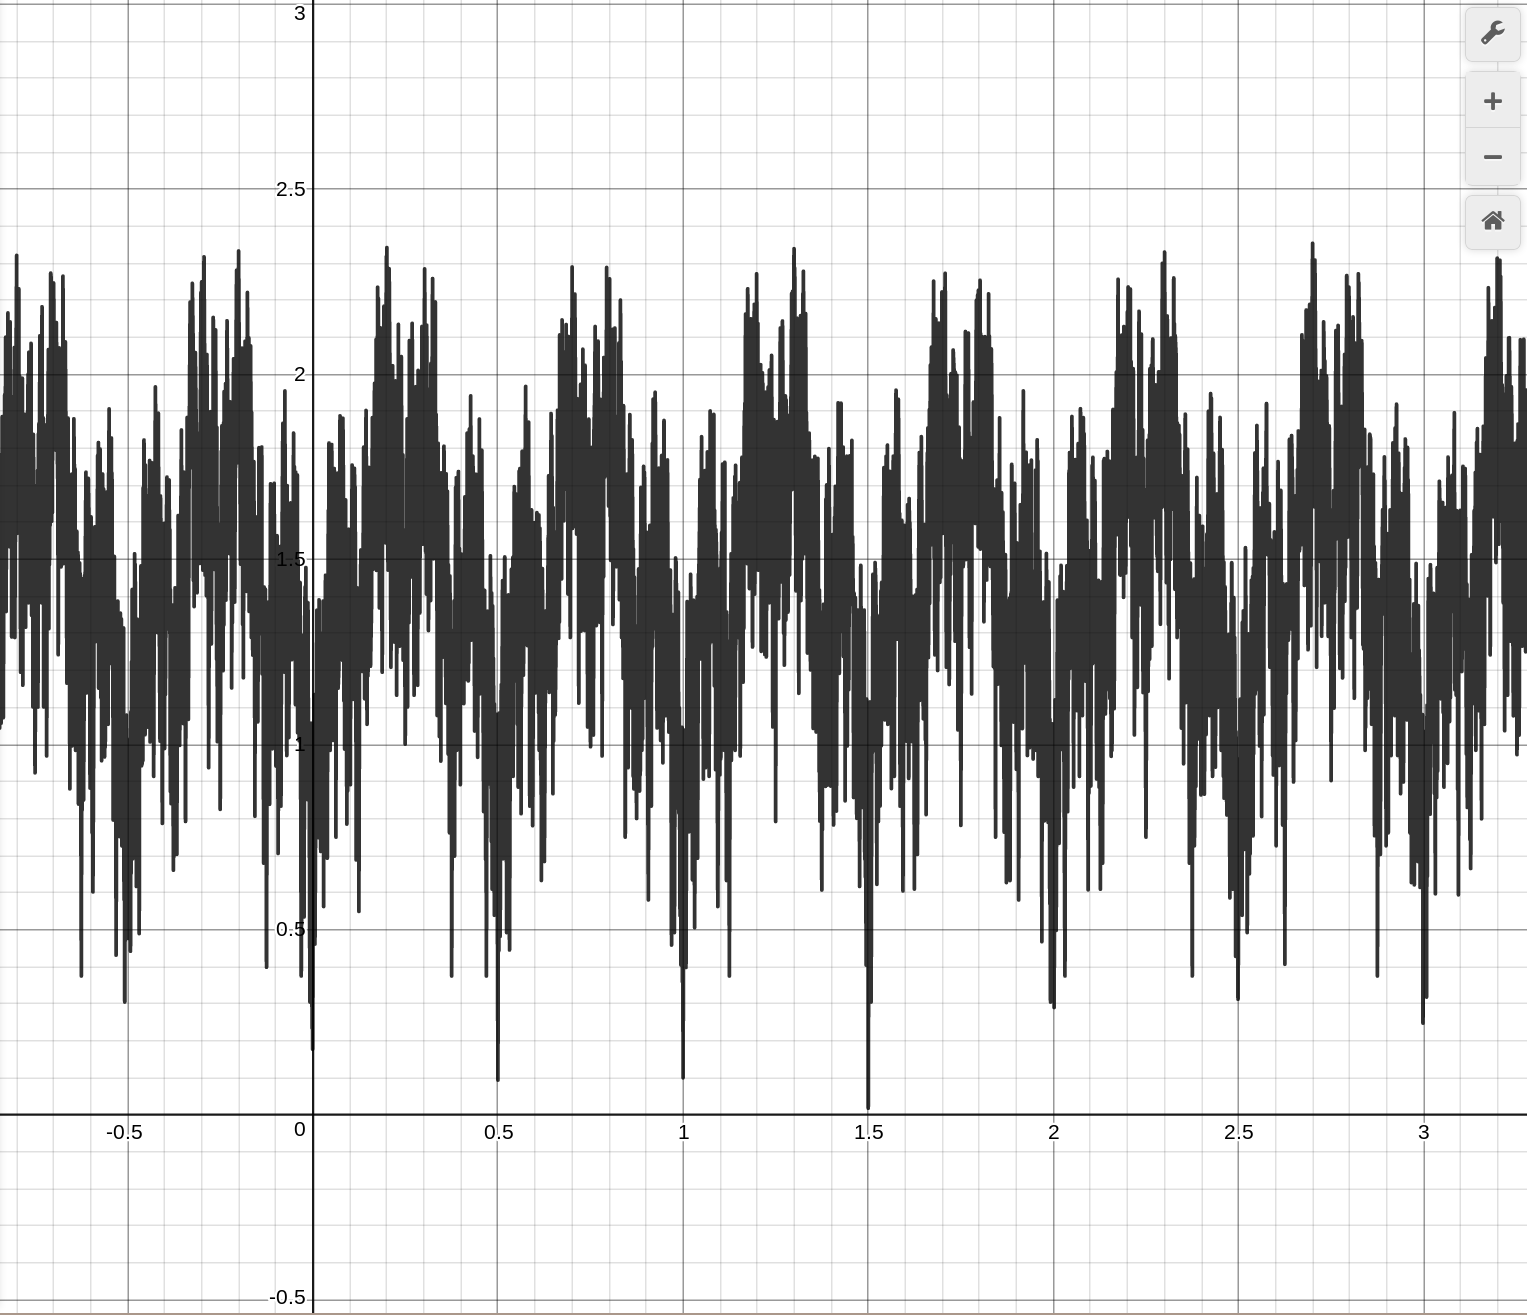
\includegraphics[width=8cm]{weierstrass.png}
    \caption{Function of $f$ as generated on Desmos. See it \href{https://www.desmos.com/calculator/rj9r0x5jyu}{live}.}\label{fig:function_of_f_as_generated_on_desmos}
    \setfloatalignment{b}% forces caption to be bottom-aligned
  \end{figure}

  \cref{fig:function_of_f_as_generated_on_desmos} is a simplified graph of $f$, drawn using the online tool \href{https://www.desmos.com}{Desmos}.

  It is clear that $\phi \in C_b(\mathbb{R})$, and $\norm{ \phi }_\infty = 1$. Thus
  \begin{equation*}
    \sum_{n=1}^{\infty} \norm{ \left( \frac{3}{4} \right)^n \phi \left( 4^n x \right)}_\infty = \sum_{n=1}^{\infty} \left( \frac{3}{4} \right)^n < \infty,
  \end{equation*}
  and so
  \begin{equation*}
    f(x) = \lim_{L \to \infty} \sum_{n=1}^{L} \left( \frac{3}{4} \right)^n \phi \left( 4^n x \right) = \lim_{L \to \infty} S_L(x),
  \end{equation*}
  uniformly so. Since the partial sums are continuous, $f \in C_b(\mathbb{R})$.

  However, $f$ is not \hlnotea{differentiable}. Let $x \in \mathbb{R}$. For each $m \in \mathbb{N}$, we can find $k \in \mathbb{Z}$ such that
  \begin{equation*}
    k \leq 4^m x \leq k + 1.
  \end{equation*}
  Let
  \begin{equation*}
    p_m = \frac{k}{4^m} \text{ and } q_m = \frac{k + 1}{4^m},
  \end{equation*}
  and for any $n \in \mathbb{N}$,
  \begin{equation*}
    \alpha = 4^n p_m = 4^{n - m} k \text{ and } \beta = 4^n q_m = 4^{ n - m } ( k + 1 ).
  \end{equation*}
  Now
  \begin{itemize}
    \item if $n > m$, then since $\alpha$ and $\beta$ differ by an even integer, $\abs{ \phi ( \alpha ) - \phi ( \beta ) } = 0$;
    \item if $n = m$, then $\alpha$ and $\beta$ differs by $1$, and so $\abs{ \phi(\alpha) - \phi(\beta) } = 1$;
    \item if $n < m$, then there are no integers between $\alpha$ and $\beta$, and so
      \begin{equation*}
        \abs{ \phi(\alpha) - \phi(\beta) } = \abs{ 4^n p_m - 4^n q_m } \footnotemark = \abs{ 4^{n - m} k - 4^{n - m} ( k + 1 ) } = 4^{n - m}.
      \end{equation*}
      \footnotetext{Note that if we have $1 \leq \alpha, \beta \leq 2$, we still get the same formula.}
  \end{itemize}

  For large enough $m$, consider
  \begin{align}
    \abs{ f\left( p_m \right) - f \left( q_m \right) }
      & = \abs{ \sum_{n=1}^{\infty} \left( \frac{3}{4} \right)^n \left( \phi \left( 4^n p_m \right) - \phi \left( 4^n q_m \right) \right) } \nonumber \\
      &= \abs{ \sum_{n=1}^{m} \left( \frac{3}{4} \right)^n \left( \phi \left( 4^n p_m \right) - \phi \left( 4^n q_m \right) \right) } \label{eq:weierstrass_fn_eq1} \\
      &\geq \abs{ \left( \frac{3}{4} \right)^n - \sum_{n=1}^{m - 1} \left( \frac{3}{4} \right)^n \abs{ \phi \left( 4^n p_m \right) - \phi \left( 4^n q_m \right) } } \label{eq:weierstrass_fn_eq2} \\
      &= \abs{ \left( \frac{3}{4} \right)^n - \sum_{n=1}^{m - 1} \left( \frac{3}{4} \right)^n 4^{n - m} } \label{eq:weierstrass_fn_eq3} \\
      &= \abs{ \left( \frac{3}{4} \right)^n - \frac{1}{4^m} \sum_{n=1}^{m - 1} 3^n } \nonumber \\
      &= \abs{ \left( \frac{3}{4} \right)^n - \frac{1}{4^m} \left[ \frac{3^m - 1}{2} \right] } \label{eq:weierstrass_fn_eq4} \\
      &= \frac{1}{4^m} \left[ \frac{3^m + 1}{2} \right] > \frac{1}{2} \cdot \left( \frac{3}{4} \right)^m \nonumber
  \end{align}
  where we note that
  \begin{itemize}
    \item[\eqref{eq:weierstrass_fn_eq1}] terms after $m$ are eliminated as they are $0$ as argued previously;
    \item[\eqref{eq:weierstrass_fn_eq2}] by the reverse Triangle ineq. and the case where $n = m$;
    \item[\eqref{eq:weierstrass_fn_eq3}] using the argument for when $n < m$;
    \item[\eqref{eq:weierstrass_fn_eq4}] using the formula for a finite geometric sum.
  \end{itemize}
  Hence we observe that
  \begin{equation*}
    \frac{\abs{ f(p_m) - f(q_m) }}{\abs{ p_m - q_m }} > 4^m \cdot \frac{3^m}{2 \cdot 4^m} = \frac{3^m}{2}.
  \end{equation*}
  Now if $p_m = x$, then
  \begin{equation*}
    \frac{\abs{ f(x) - f(q_m) }}{\abs{ x - q_m }} > \frac{3^m}{2}.
  \end{equation*}
  If $p_m \neq x$, then
  \begin{align*}
    \frac{3^m}{2} &< \frac{\abs{ f(p_m) - f(q_m) }}{\abs{ p_m - q_m }} \leq \frac{\abs{ f(p_m) - f(x) } + \abs{ f(x) - f(q_m) }}{\abs{ p_m - q_m }} \\
                  &\leq \frac{\abs{ f(p_m) - f(x) }}{\abs{ p_m - x }} + \frac{\abs{ f(x) - f(q_m) }}{\abs{ x - q_m }},
  \end{align*}
  which implies that either
  \begin{equation*}
    \frac{\abs{ f(x) - f(q_m) }}{\abs{ x - q_m }} > \frac{3^m}{2},
  \end{equation*}
  or
  \begin{equation*}
    \frac{\abs{ f(p_m) - f(x) }}{\abs{ p_m - x }} > \frac{3^m}{2}.
  \end{equation*}
  Then for any sequence $\{ t_m \}$ such that $t_m \to x$, and $t_m \neq x$, we have that
  \begin{equation*}
    \frac{\abs{ f(x) - f(t_m) }}{\abs{ x - t_m }} \geq \frac{3^m}{4} \to \infty
  \end{equation*}
  as $m \to \infty$. Thus the function $f$ is not differentiable at any $x$.
\end{eg}

% subsection characterizations_of_completeness_continued_2 (end)

% section completeness_of_metric_spaces_continued_4 (end)

% chapter lecture_23_nov_05th (end)

\chapter{Lecture 24 Nov 07th}%
\label{chp:lecture_24_nov_07th}
% chapter lecture_24_nov_07th

\section{Completions of Metric Spaces}%
\label{sec:completions_of_metric_spaces}
% section completions_of_metric_spaces

\begin{defn}[Isometry]\index{Isometry}\label{defn:isometry}
  A map $\phi : (X, d_X) \to (Y, d_Y)$ is called an \hlnoteb{isometry} if
  \begin{equation*}
    d_Y( \phi(x_1), \phi(x_2) ) = d_X(x_1, x_2).
  \end{equation*}
\end{defn}

\begin{defn}[Completion]\index{Completion}\label{defn:completion}
  A \hlnoteb{completion} of a metric space $(X, d)$ is a pair $\left( \left(Y, d_Y\right), \phi \right)$ where $\left(Y, d_Y\right)$ is a complete metric space, $\phi : X \to Y$ is an isometry, and $\bar{\phi(X)} = Y$.
\end{defn}

\begin{propo}[Subsets of Complete Spaces are Complete if they are Closed]\label{propo:subsets_of_complete_spaces_are_complete_if_they_are_closed}
  Let $(X, d)$ be a complete metric space. Let $A \subset X$. Then $(A, d_A)$ is complete iff $A$ is closed.
\end{propo}

\begin{proof}
  \hlbnoted{$(\implies)$}: $(A, d_A)$ is complete \\
  $\implies \{ x_n \} \subset A$ Cauchy $\implies x_n \to x_0$
  $\implies x_0 \in A \implies \Lim(A) \subseteq A$ \\
  $\implies A$ is closed.

  \noindent
  \hlbnoted{$(\impliedby)$} Let $\{ x_n \} \subset A$ be Cauchy in $(A, d_A)$ \\
  $\implies \{ x_n \}$ is Cauchy in $(X, d)$ \\
  $\implies x_n \to x_0 \in X$ \\
  $\implies (\because A \text{ is closed }) x_0 \in A$ \\
  $\implies (A, d_A)$ is complete.\qed\
\end{proof}

A natural question arises: does every space have a completion?

To answer this, we need the following concept:

\begin{defn}[Uniformly Continuous Functions]\index{Uniform Continuity}\label{defn:uniformly_continuous_functions}
  We say that a function $f : (X, d_X) \to (Y, d_Y)$ is \hlnoteb{uniformly continuous} if
  \begin{gather*}
    \forall \epsilon > 0 \; \exists \delta > 0 \; \forall x_1, x_2 \in X \\
    d_X(x_1, x_2) < \delta \implies d_Y \left( f(x_1) , f(x_2) \right) < \epsilon.
  \end{gather*}
\end{defn}

\begin{eg}
  Given $(X, d)$, and $x_0 \in X$, define
  \begin{equation*}
    g_{x_0}(x) = d(x, x_0).
  \end{equation*}
  Note that $\abs{ d(x_0, x) - d(x_0, y) } \leq d(x, y)$.\sidenote{Proved in A3} Thus
  \begin{equation*}
    \abs{ g_{x_0}(x_1) - g_{x_0}(x_2) } \leq d(x_1, x_2).
  \end{equation*}
  Then $\forall \epsilon > 0 \; \exists \delta = \epsilon > 0$, we have
  \begin{equation*}
    d(x_1, x_2) < \delta \implies \abs{ g_{x_0}(x_1) - g_{x_0}(x_2) } < \epsilon.
  \end{equation*}
  Thus $g_{x_0}$ is uniformly continuous.
\end{eg}

\begin{thm}[Completion Theorem]\index{Completion Theorem}\label{thm:completion_theorem}
  Every metric space $(X, d)$ has a completion.
\end{thm}

\begin{proof}
  Let $a \in X$. Define $\phi : X \to C_b(X)$ by
  \begin{equation*}
    \left( \phi(u) \right)(x) = f_u(x) = d(u, x) - d(x, a).
  \end{equation*}
  By our earlier example, $\phi(u)$ is continuous. Notice that we have
  \begin{equation*}
    \abs{ f_u(x) } = \abs{ d(u, x) - d(x, a) } \leq d(u, a).
  \end{equation*}
  Thus $\phi(u) in C_b(X)$, proving that $\phi$ is well-defined.

  WTS $\phi$ is an isometry. Let $u, v \in X$. Then
  \begin{align*}
    \abs{ f_u(x) - f_v(x) } &= \abs{ d(u, x) - d(x, a) - d(v, x) - + d(x, a) } \\
                            &= \abs{ d(u, x) - d(v, x) } \\
                            &\leq d(u, v).
  \end{align*}
  Thus $\norm{ f_u - f_v }_\infty \leq d(u, v)$ by definition of $\norm\cdot_\infty$. Notice that
  \begin{equation*}
    \abs{ f_u(v) - f_v(v) } = d(u, v),
  \end{equation*}
  which gives us the greatest possible value. Thus
  \begin{equation*}
    \norm{ \phi(u) - \phi(v) }_\infty = \norm{ f_u - f_v }_\infty = d(u, v).
  \end{equation*}
  Thus $\phi$ is an isometry.

  Since $(C_b(X), \norm\cdot_\infty)$ is a complete metric space, let $Y = \bar{\phi(X)}$. The proof is complete by \cref{propo:subsets_of_complete_spaces_are_complete_if_they_are_closed}.\qed\
\end{proof}

\newthought{Question}: If $(X, d)$ has 2 completions, how are they related?

Suppose $(X, d)$ is a metric space that has 2 completions through the functions $\phi$ and $\psi$.

\begin{figure}[!ht]
  \centering
  \begin{tikzpicture}
    \node (X) at (0,0) {$X$};
    \draw (X) circle(1);
    \node (phiX) at (3,1) {$\phi(X)$};
    \draw (phiX) circle(1);
    \node (psiX) at (2,-2) {$\psi(X)$};
    \draw (psiX) circle(1);

    \draw[->] (0.5, 0.5) -- (2.5, 1) node[midway,above] {$\phi$};
    \draw[->] (0.5, -0.5) -- (1.5, -1.5) node[midway,below,left] {$\psi$};
  \end{tikzpicture}
  \caption{Relation of the 2 completions of a metric space.}
  \label{fig:relation_2_completions_metric_space}
\end{figure}

Since we have that $\phi$ is bijective from $X$ to $\phi(X)$, we can take its inverse. Consequently, we have that the function $\Gamma = \psi \circ \phi^{-1}$ is an isometry.

Now for some $\{ x_n \} \subset X$ that is Cauchy, we know that in $\phi(X)$, $\phi(x_n) \to y_0 \in \phi(X)$. Note that $y_0$ is a limit point of $\phi(X)$. Through $\Gamma$, we have that
\begin{equation*}
  \Gamma( \phi(x_n) ) = \psi( x_n ).
\end{equation*}
If $\psi(x_n) \to z_0 \in \psi(X)$, then we must have
\begin{equation*}
  \Gamma(y_0) = z_0,
\end{equation*}
and in particular $z_0$ is a limit point of $\psi(X)$. This forces limits point of $\phi(X)$ to also be limit points of $\psi(X)$, and interior to interior. Thus the two completions are isomorphic.

% section completions_of_metric_spaces (end)

\section{Banach Contractive Mapping Theorem}%
\label{sec:banach_contractive_mapping_theorem}
% section banach_contractive_mapping_theorem

\newthought{Question}: Does there exist a function $f \in C[0, 1]$ such that
\begin{equation}\label{eq:weird_looking_function}
  f(x) = e^x + \int_{0}^{x} \frac{\sin t}{2} f(t) \dif{t} \quad ?
\end{equation}

Let $\Gamma : C[0, 1] \to C[0, 1]$ such that
\begin{equation*}
  \Gamma (f) (x) = e^x + \int_{0}^{x} \frac{\sin t}{2} f(t) \dif{t}.
\end{equation*}
Then $f_0$ is a solution to \cref{eq:weird_looking_function} iff $\Gamma(f_0) = f_0$.

This is known as an \hlnotea{integral transform}.

\begin{defn}[Fixed Point]\index{Fixed Point}\label{defn:fixed_point}
  Given $(X, d)$, $\Gamma : X \to X$, we say that $x_0$ is a fixed point of $\Gamma$ if $\Gamma(x_0) = x_0$.
\end{defn}

% section banach_contractive_mapping_theorem (end)

% chapter lecture_24_nov_07th (end)

\chapter{Lecture 25 Nov 09th}%
\label{chp:lecture_25_nov_09th}
% chapter lecture_25_nov_09th

\section{Banach Contractive Mapping Theorem (Continued)}%
\label{sec:banach_contractive_mapping_theorem_continued}
% section banach_contractive_mapping_theorem_continued

\begin{defn}[Lipschitz]\index{Lipschitz}\label{defn:lipschitz}
  A function $f : (X, d_X) \to (Y, d_Y)$ is said to be Lipschitz if there exists $\alpha \geq 0$ such that $\forall x_1, x_2 \in X$,
  \begin{equation*}
    d_Y( f(x_1), f(x_2) ) \leq \alpha d_X(x_1, x_2)
  \end{equation*}
\end{defn}

\begin{defn}[Contraction]\index{Contraction}\label{defn:contraction}
  A function $f : X \to Y$ is called a \hlnoteb{contraction} if there exists $0 \leq k < 1$ with
  \begin{equation*}
    d_Y( f(x_1), f(x_2) ) \leq k d_X(x_1, x_2)
  \end{equation*}
  for all $x_1, x_2 \in X$.
\end{defn}

\begin{note}
  Notice that a Lipschitz function is uniformly continuous: choose $\delta = \frac{\epsilon}{\alpha}$.
\end{note}

\begin{ex}
  Prove that if $f : [a, b] \to \mathbb{R}$ and $f'$ is continuous, then by the \hlnotea{Extreme Value Theorem} and the \hlnotea{Mean Value Theorem}, $f$ is Lipschitz.
\end{ex}

\begin{thm}[Banach Contractive Mapping Theorem]\index{Banach Contractive Mapping Theorem}\label{thm:banach_contractive_mapping_theorem}
  Assume that $(X, d)$ is complete. If $\Gamma : X \to X$ is contractive, then there exists a unique $x_0 \in X$ such that $\Gamma (x_0) = x_0$.
\end{thm}

\begin{proof}
  Pick $x_1 \in X$. Then, let
  \begin{equation*}
    x_2 = \Gamma(x_1), \, x_3 = \Gamma(x_2), \, \ldots , \, x_{n + 1} = \Gamma(x_n), \, \ldots .
  \end{equation*}

  \noindent
  \hlbnoted{Claim}: $\{ x_n \}$ is Cauchy\sidenote{This will CTP since $(X, d)$ is complete, i.e. it will give us a limit point at which $\Gamma$ must converge to, and thus forcing its iteration to be terminated at the limit point due to $\Gamma$ being contractive.}

  Let $k \in \mathbb{R}$ such that $0 < k < 1$, so that we have
  \begin{equation*}
    d \left( \Gamma(x), \Gamma(y) \right) \leq k d(x, y)
  \end{equation*}
  for any $x, y \in X$. Then
  \begin{align*}
    d(x_3, x_2) &= d( \Gamma(x_2), \Gamma(x_1) ) \leq k d(x_2, x_1) \\
    d(x_4, x_3) &= d( \Gamma(x_3), \Gamma(x_1) ) \leq k d(x_3, x_2) \leq k^2 d(x_2, x_1) \\
                & \vdots \\
    d(x_{n + 1}, x_n) &= d( \Gamma(x_{n + 1}), \Gamma(x_n) ) \leq k^{n - 1} d(x_2, x_1) \\
                      & \vdots
  \end{align*}
  Also, notice that if $m > n$, then
  \begin{align*}
    d(x_m, x_n) &\leq d(x_m, x_{m - 1}) + d(x_{m - 1}, x_{m - 2}) + \hdots + d(x_{n + 1}, x_n) \\
                &\leq k^{m - 2} d(x_2, x_1) + k^{m - 3} d(x_2, x_1) + \hdots + k^{n - 1} d(x_2, x_1) \\
                &= \sum_{j=n-1}^{m-2} k^j d(x_2, x_1) = \frac{k^{n - 1}}{1 - k} d(x_2, x_1).
  \end{align*}
  Since $k^{n - 1} \to 0$, we have that $\{ x_n \}$ is Cauchy. Since $(X, d)$ is complete, $\exists x_0 \in X$ such that $x_n \to x_0$.

  In particular, we have that $x_{n + 1} \to x_0$, i.e. $\Gamma(x_n) \to x_0$. Since $\Gamma$ is continuous, we mst have that $\Gamma(x_n) \to \Gamma(x_0)$. Therefore $\Gamma(x_0) = x_0$ as required.

  \hlbnotea{(Uniqueness)} Suppose there exists another point $y_0 \in X$ such that $\Gamma(y_0) = y_0$. Then
  \begin{equation*}
    d(x_0, y_0) = d(\Gamma(x_0), \Gamma(y_0)) \leq kd(x_0, y_0),
  \end{equation*}
  which implies that $d(x_0, y_0) = 0$.\qed\
\end{proof}

\begin{eg}
  Show that the equation
  \begin{equation*}
    f_0(x) = e^{x} + \int_{0}^{x} \frac{\sin t}{2}f_0(t) \dif{t}
  \end{equation*}
  has a unique solution in $C[0, 1]$.
\end{eg}

\begin{solution}
  Define $\Gamma : C[0, 1] \to C[0, 1]$ by
  \begin{equation*}
    \Gamma(f)(x) = e^x + \int_{0}^{x} \frac{\sin t}{2} f(t) \dif{t}.
  \end{equation*}
  Let $f, g \in C[0, 1]$. We have that
  \begin{align*}
    \abs{ \Gamma(f)(x) - \Gamma(g)(x) }
      &= \abs{ \int_{0}^{x} \frac{\sin t}{2} f(t) \dif{t} - \int_{0}^{x} \frac{\sin t}{2} g(t) \dif{t} } \\
      &= \abs{ \int_{0}^{x} \frac{\sin t}{2} \left( f(t) - g(t) \right) \dif{t} } \\
      &\leq \int_{0}^{x} \abs{ \frac{\sin t}{2} } \abs{ f(t) - g(t) } \dif{t} \\
      &\leq \norm{ f - g }_\infty \int_{0}^{1}  \frac{1}{2} \dif{t} \\
      &= \frac{1}{2} \norm{ f - g }_\infty
  \end{align*}
  Thus $\norm{ \Gamma(f) - \Gamma(g) }_\infty \leq \frac{1}{2} \abs{ f - g }_\infty$. Thus $\Gamma$ is contractive. By \cref{thm:banach_contractive_mapping_theorem}, the unique fixed point is the solution.
\end{solution}

\begin{eg}
  Show that the equation
  \begin{equation}\label{eq:banach_contractive_map_eg2}
    f(x) = x + \int_{0}^{x} t^2 f(t) \dif{t}
  \end{equation}
  has a unique solution.
\end{eg}

\begin{solution}
  Let $\Gamma(f)(x) = x + \int_{0}^{x} t^2 f(t) \dif{t}$. Then
  \begin{align*}
    \abs{ \Gamma(f)(x) - \Gamma(g)(x) } &= \leq \int_{0}^{1} t^2 \norm{ f - g }_\infty \dif{t}  \\
                                        &= \frac{1}{3}\norm{ f - g }_\infty.
  \end{align*}
  By the Banach Contractive Mapping Theorem, \cref{eq:banach_contractive_map_eg2} has a unique solution. In particular,
  \begin{align*}
    f_1(x) &= x \\
    f_2(x) &= \Gamma(f_1)(x) = x + \int_{0}^{x} t^2 t_1(t) \dif{t} \\
           &= x + \int_{0}^{x} t^3 \dif{t} = x + \frac{1}{4}x^4 \\
    f_3(x) &= \Gamma(f_2)(x) = x + \int_{0}^{x} t^2 \left( t + \frac{1}{4} t^4 \right) \dif{t} \\
           &= x + \int_{0}^{x} t^3 + \frac{1}{4} t^6 \dif{t} = x + \frac{1}{4} x^4 + \frac{1}{4 \cdot 7} x^7 \\
           &\vdots \\
    f_n(x) &= \frac{x}{1} + \frac{x^4}{4} + \frac{x^7}{4 \cdot 7} + \hdots + \frac{x^{3n - 2}}{4 \cdot 7 \cdot \hdots \cdot (3n - 2)}
  \end{align*}
  and so the limit is
  \begin{equation*}
    f_0(x) = \sum_{k=1}^{\infty} \frac{x^{3k - 2}}{4 \cdot 7 \cdot \hdots \cdot (3k - 2)}.
  \end{equation*}
\end{solution}

\begin{eg}[Other Applications]
  \begin{enumerate}
    \item \href{https://en.wikipedia.org/wiki/Newton%27s_method}{Newton's Method}.
      \item (\hldefn{Picard's Theorem}) Let $f : [a, b] \times \mathbb{R} \to \mathbb{R}$ be Lipschitz in $\mathbb{R}$, i.e. $\exists \alpha \geq 0$ such that
        \begin{equation*}
          \abs{ f(t, y_1) - f(t, y_2) } \leq \alpha \abs{ _1 - y_2 }
        \end{equation*}
        for any $y_1, y_2 \in \mathbb{R}$. If $y_0 \in \mathbb{R}$, then there exists a unique $\phi \in C[a, b]$ such that
        \begin{equation*}
          \phi'(t) = f(t, \phi(t))
        \end{equation*}
        for all $t \in (a, b)$ with $\phi(a) = y_0$.
  \end{enumerate}
\end{eg}

% section banach_contractive_mapping_theorem_continued (end)

\section{Baire Category Theorem}%
\label{sec:baire_category_theorem}
% section baire_category_theorem

\begin{eg}[Dirchlet Function]
  Consider the function
  \begin{equation*}
    f(x) = \begin{cases}
      0           & x \in \mathbb{R} \setminus \mathbb{Q}\\
      1           & x = 0 \\
      \frac{1}{m} & x \in \mathbb{Q}
    \end{cases}
  \end{equation*}
  The function $g$ is continuous at each $x \in \mathbb{R} \setminus \mathbb{Q}$, and discontinuous otherwise.
\end{eg}

\newthought{Question}: Does there exist a function function $f$ such that $f$ is continuous on $\mathbb{Q}$ but not on $\mathbb{R} \setminus \mathbb{Q}$? \hlimpo{No!}

However, to prove that there is need no such function, we need more machinery. In particular, the set of discontinuities of a function $f : (X, d) \to \mathbb{R}$ has a particular topological nature.

\begin{defn}[Points of Discontinuity]\index{Points of Discontinuity}\label{defn:points_of_discontinuity}
  Let $f : X \to \mathbb{R}$. For each $n \in \mathbb{N}$, the \hlnoteb{points of discontinuity} is a set defined as
  \begin{equation*}
    D_N(f) = \left\{ x_0 \in X : \forall \delta > 0 \; \exists x_1, y_1 \in B(x_0, \delta) \; \abs{ f(x_1) - f(y_1) } \geq \frac{1}{n} \right\}.
  \end{equation*}
\end{defn}

\begin{note}
  \begin{enumerate}
    \item For each $n \in \mathbb{N}$, $D_n$ is closed.
    \item $f$ is continuous at $x_0 \iff x_0 \notin \bigcap_{n = 1}^{\infty} D_n$.
  \end{enumerate}
\end{note}

\begin{remark}
  Recall the definition of an $F_\sigma$-set from the midterm (definition also provided in next lecture).

  The set
  \begin{equation*}
    D(f) = \{ x_0 \in X \mid f \text{ is discontinuous at } x_0 \} = \bigcap_{n = 1}^{\infty} D_n(f)
  \end{equation*}
  is an $F_\sigma$-set.
\end{remark}

A natural question to ask is:

\newthought{Question}: Is $\mathbb{R} \setminus \mathbb{Q}$ an $F_\sigma$-set?

% section baire_category_theorem (end)

% chapter lecture_25_nov_09th (end)

\chapter{Lecture 26 Nov 12th}%
\label{chp:lecture_26_nov_12th}
% chapter lecture_26_nov_12th

\section{Baire Category Theorem (Continued)}%
\label{sec:baire_category_theorem_continued}
% section baire_category_theorem_continued

\begin{defn}[$F_\sigma$ Sets]\index{$F_\sigma$ Sets}\label{defn:_f_sigma_sets}
  Let $(X, d)$ be a metric space. We say that $A \subseteq X$ is \hlnoteb{$F_\sigma$} if there exists a sequence $\{ F_n \}_{n = 1}^{\infty}$ of closed sets with
  \begin{equation*}
    A = \bigcup_{n=1}^{\infty} F_n.
  \end{equation*}
\end{defn}

\begin{defn}[$G_\delta$ Sets]\index{$G_\delta$ Sets}\label{defn:_g_delta_sets}
  Let $(X, d)$ be a metric space. We say that $A \subseteq X$ is \hlnoteb{$G_\delta$} if there exists a sequence $\{ U_n \}_{n = 1}^{\infty}$ of open sets such that
  \begin{equation*}
    A = \bigcap_{n=1}^{\infty} U_n.
  \end{equation*}
\end{defn}

\begin{eg}
  The interval $[0, 1) \subset \mathbb{R}$ is $G_\delta$, since
  \begin{equation*}
    [0, 1) = \bigcap_{n=1}^{\infty} \left( \frac{1}{n}, 1 \right)
  \end{equation*}
\end{eg}

\begin{remark}
  $A$ is $F_\sigma$ iff $A^C$ is $G_\delta$.
\end{remark}

Recall the definition of a \hyperref[defn:dense]{dense set}. We have the following complementary definition.

\begin{defn}[Nowhere Dense]\index{Nowhere Dense}\label{defn:nowhere_dense}
  Given a metric space $(X, d)$, we say that $A \subseteq X$ is \hlnoteb{nowhere dense} if $\bar{A}^\circ = \emptyset$.
\end{defn}

\begin{remark}
  The above definition is equivalent to saying that $\bar{A}^C$ is dense.
\end{remark}

\begin{defn}[First Category]\index{First Category}\label{defn:first_category}
  We say that a set $A$ is of \hlnoteb{first category} if
  \begin{equation*}
    A = \bigcup_{n=1}^{\infty} A_n
  \end{equation*}
  where each $A_n$ is nowhere dense.
\end{defn}

\begin{defn}[Second Category]\index{Second Category}\label{defn:second_category}
  We say that $A$ is of \hlnoteb{second category} is $A$ is not of first category.
\end{defn}

\begin{remark}
  We colloquially refer to a set of first category as being \hlnotea{topologically thin}, and a set of second category as being \hlnotea{topologically thick}.
\end{remark}

\begin{defn}[Residual]\index{Residual}\label{defn:residual}
  We say that $A \subseteq (X, d)$ is a \hlnoteb{residual} in $X$ if $A^C$ is of first category.
\end{defn}

\begin{thm}[Set of Points of Discontinuity is $F_\sigma$]\label{thm:set_of_points_of_discontinuity_is_f_sigma_}
  Let $f : (X, d_X) \to (Y, d_Y)$. Then for each $n \in \mathbb{N}$, $D_N(f)$ is closed in $X$. Moreover,
  \begin{equation*}
    D(f) = \bigcup_{n=1}^{\infty} D_N(f).
  \end{equation*}
  In particular, $D(f)$ is $F_\sigma$.
\end{thm}

\begin{ex}
  Prove \cref{thm:set_of_points_of_discontinuity_is_f_sigma_}.
\end{ex}

\begin{eg}
  If $F \subset (X, d)$ is closed, then $f$ is $G_\delta$. In particular, notice that
  \begin{equation*}
    F = \bigcap_{n=1}^{\infty} \left( \bigcup_{x \in F} B \left( x, \frac{1}{n} \right) \right),
  \end{equation*}
  where we note that each of the $B \left( x, \frac{1}{n} \right)$ is $F_\delta$.
\end{eg}

\begin{thm}[Baire Category Theorem I]\index{Baire Category Theorem I}\label{thm:baire_category_theorem_i}
  Let $(X, d)$ be complete. Let $\{ U_n \}_{n = 1}^{\infty}$ be a countable collection of dense open sets. Then\sidenote{Note that we have ourselves a dense $G_\delta$ set.}
  \begin{equation*}
    \bigcap_{n=1}^{\infty} U_n \text{ is dense in } X.
  \end{equation*}
  In particular, it is not empty.
\end{thm}

\begin{proof}
  Assume that $\{ U_n \}_{n = 1}^{\infty}$ is a sequence of open and dense sets. Let $W \subset X$ be open and non-empty. Since $U_1$ is dense, we have that $W \cap U_1 \neq \emptyset$. Then $\exists x_1 \in W \cap U_1$ such that $\exists 0 < r_1 \leq 1$ so that
  \begin{equation*}
    B(x_1, r_1) \subset B(x_1, r_1) \subset W \cap U_1.
  \end{equation*}
  Similarly,
  \begin{marginfigure}
    \centering
    \begin{tikzpicture}
      \draw (0, 0) circle(1) node[above,left] at (-0.5, 1) {$W$};
      \draw (0.5,-0.5) circle(1) node[below,right] at (1.5, -0.5) {$U_1$};
      \draw[dashed] (0.3,-0.3) circle(0.5) node {$B(x_1, r_1)$};
    \end{tikzpicture}
    \caption{Visualization of proof for Baire Category Theorem I}\label{fig:visualization_of_proof_for_baire_category_theorem_i}
  \end{marginfigure}
  we can find $x_2 \in X$ such that for some $0 < r_2 \leq \frac{1}{2}$,
  \begin{equation*}
    B ( x_2 , r_2 ) \subset B [ x_2, r ] \subset B(x_1, r_1) \cap U_2.
  \end{equation*}
  We can proceed recursively and find, for $n \in \mathbb{N}$, an $x_{n} \in X$ with $0 < r_{n} \leq \frac{1}{n}$ such that
  \begin{equation*}
    B ( x_n, r_n ) \subset B [ x_n, r_n ] \subset B ( x_{n - 1}, r_{n - 1} ) \cap U_{n}.
  \end{equation*}
  Now since $(X, d)$ is complete, $\{ \diam( B [x_n, r_n] ) \} = \{ r_n \}$ is a decreasing sequence such that $r_n \to 0$, by \hyperref[thm:cantor_s_intersection_principle]{Cantor's Intersection Principle},
  \begin{equation*}
    \exists x_0 \in \bigcap_{n=1}^{\infty} B[x_n, r_n].
  \end{equation*}
  Then by this construction, we must have $x_0 \in B[x_1, r_1] \subset W \cap U_1$, and $x_0 \in B[ x_n, r_n ] \subset U_n$ for each $n \in \mathbb{N}$. Thus
  \begin{equation*}
    x_0 \in W \cap \left( \bigcap_{n=1}^{\infty} U_n \right).
  \end{equation*}\qed\
\end{proof}

Note that the statement does not hold if we have an uncountable collection of dense open sets.

\begin{eg}
  Consider $U_x = \mathbb{R} \setminus \{ x \}$, where $x \in \mathbb{R}$. This is clearly a dense and open set. Notice, however, that
  \begin{equation*}
    \bigcap_{x \in \mathbb{R}} U_x = \emptyset.
  \end{equation*}
\end{eg}

\begin{remark}
  \cref{thm:baire_category_theorem_i} shows that given a countable sequence $\{ U_n \}_{n = 1}^{\infty}$ of open dense sets of $X$, the countable intersection of these sets, $\bigcap_{n=1}^{\infty} U_n$, is a dense $G_\delta$.
\end{remark}

\begin{thm}[\imponote\ Baire Category Theorem II]\index{Baire Category Theorem II}\label{thm:baire_category_theorem_ii}
  If $(X, d)$ is complete, then $X$ is of second category.
\end{thm}

\begin{proof}
  Suppose to the contrary that $X = \bigcup_{n=1}^{\infty} A_n$ where each $A_n$ is nowhere dense. Note that by definition of being nowhere dense, we have that $A_n = \bar{A_n}$. Let $U_n = \bar{A_n}^C$, which would then be open and dense. However, by \hyperref[thm:de_morgan_s_laws]{De Morgan's Laws}, we have that
  \begin{equation*}
    \left( \bigcap_{n=1}^{\infty} U_n \right)^C = \bigcup_{n=1}^{\infty} U_n^C = \bigcup_{n=1}^{\infty} \bar{A_n} = X
  \end{equation*}
  and so
  \begin{equation*}
    \bigcup_{n=1}^{\infty} U_n = \emptyset,
  \end{equation*}
  which is impossible by \cref{thm:baire_category_theorem_i}.\qed\
\end{proof}

\begin{eg}
  $\mathbb{R}$ and $\mathbb{R} \setminus \mathbb{Q}$ are of second category. In fact, $\mathbb{R} \setminus \mathbb{Q}$ is a residual, since $\mathbb{Q}$ is of first category.
\end{eg}

\newthought{Question}: Is
\begin{equation*}
  Q = \bigcap_{k=1}^{\infty} \bigcup_{n=1}^{\infty} \left( r_n - \frac{1}{2^{k + n}}, r_n + \frac{1}{2^{k + n}} \right),
\end{equation*}
where $Q = \{ r_1, r_2, \ldots \}$, $\mathbb{Q}$? No. Notice that this is fairly close, but it is not.\sidenote{It should be $\mathbb{R}$?}

\begin{crly}[$\mathbb{Q}$ is not $G_\delta$]\label{crly:_q_is_not_g_delta_}
  $\mathbb{Q}$ is not a $G_\delta$ set.
\end{crly}

\begin{proof}
  Suppose to the contrary that $\mathbb{Q}$ is $G_\delta$, i.e. there exists a countable sequence of open sets $\{ U_n \}$ such that
  \begin{equation*}
    \mathbb{Q} = \bigcap_{n=1}^{\infty} U_n.
  \end{equation*}
  Let $F_n = U_n^C$. Since $\mathbb{Q}$ is dense, it follows that each of the $U_n$'s is also dense. Thus $F_n$ is nowhere dense and closed.

  Let $\mathbb{Q} = \{ r_1, r_2, \ldots \}$, an enumeration on $\mathbb{Q}$, and $S_n = F_n \cup \{ r_n \}$. Then $S_n$ is closed and nowhere dense. However, we would then have
  \begin{equation*}
    \mathbb{R} = \bigcup_{n=1}^{\infty} S_n,
  \end{equation*}
  which contradicts the fact that $\mathbb{R}$ is of second category.\qed\
\end{proof}

Consequently:

\begin{crly}[There are no Functions Discontinuous on all Irrational Numbers]\label{crly:there_are_no_functions_discontinuous_on_all_irrational_numbers}
  There is no function $f : \mathbb{R} \to \mathbb{R}$ for which $D(f) = \mathbb{R} \setminus \mathbb{Q}$.
\end{crly}

We are now able to show that for a sequence $\{ f_n \} \subset C[a, b]$ that converges pointwise, the limit function must be continuous at each point on a residual set. We require the following notion:

\begin{defn}[Uniformly Convergent Sequence of Functions on a Point]\label{defn:uniformly_convergent_sequence_of_functions_on_a_point}
  We say that a sequence of functions $\{ f_n \}$ where,
  \begin{equation*}
    f_n : (X, d_X) \to (Y, d_Y),
  \end{equation*}
  \hlnoteb{converges uniformly} at $x_0 \in X$ if
  \begin{gather*}
    \forall \epsilon > 0 \; \exists \delta > 0 \; \exists N \in \mathbb{N} \; \forall n, m \geq N \\
    x \in B(x_0, \delta) \implies d_Y(f_n(x), f_m(x)) < \epsilon.
  \end{gather*}
\end{defn}

The proof of the following theorem is left as an exercise.

\begin{thm}[Limit of Sequence of Continuous Functions that Converges Pointwise is Continuous]\label{thm:limit_of_sequence_of_continuous_functions_that_converges_pointwise_is_continuous}
  Let $(X, d_X)$ and $)Y, d_Y)$ be metric spaces. Let $\{ f_n : X \to Y \}$ be a sequence of functions that converges pointwise on $X$ to $f_0$. Assume that $\{ f_n \}$ converges uniformly at $x_0 \in X$. If each $f_n$ is continuous at $x_0$, then so is $f_0$.
\end{thm}

% section baire_category_theorem_continued (end)

% chapter lecture_26_nov_12th (end)

\chapter{Lecture 27 Nov 14th}%
\label{chp:lecture_27_nov_14th}
% chapter lecture_27_nov_14th

\section{Baire Category Theorem (Continued 2)}%
\label{sec:baire_category_theorem_continued_2}
% section baire_category_theorem_continued_2

\begin{thm}[Uniform Convergence of A Sequence of Continuous Functions that Converges Pointwise]\label{thm:uniform_convergence_of_a_sequence_of_continuous_functions_that_converges_pointwise}
  Let $f_n : (a, b) \to \mathbb{R}$ be a sequence of continuous functions that converges pointwise to $f(x)$. Then there exists an $x_0 \in (a, b)$ such that $f_n \to f$ uniformly at $x_0$.
\end{thm}

\begin{proof}
  Assume that $f_n \to f_0$ on $(a, b)$, pointwise.

  \noindent
  \hlbnoted{Claim} There exists $[ \alpha_1, \beta_1 ] \subset (a, b)$ and $N_1 \in \mathbb{N}$ such that if $x \in [\alpha_1, \beta_1]$ and $n, m \geq N_1$, then $\abs{ f_n(x) - f_m(x) } \leq 1$.

  \noindent
  Suppose not. Then $\exists t_1 \in (a, b)$ and $n_1, m_1 \in \mathbb{N}$ such that \\
  \noindent
  $\abs{ f_{n_1}(t_1) - f_{m_1}(t_1) } > 1$. Since $f_{n_1} - f_{m_1}$ is continuous, there exists an open interval $I_1 \subsetneq \bar{I}_1 \subsetneq (a, b)$ such that $\abs{ f_{n_1}(x) - f_{m_1}(x) } > 1$ for all $x \in I_1$.

  Similarly, $\exists t_2 \in I_1$ and $n_2, m_2 \geq \max \{ n_1, m_1 \}$ such that \\
  \noindent
  $\abs{ f_{n_2}(t_2) - f_{m_2}(t_2) } > 1$. Again, since $f_{n_2} - f_{m_2}$ is continuous, there exists an open interval $I_2 \subsetneq \bar{I}_2 \subsetneq I_1$ such that $\abs{ f_{n_2}(x) - f_{m_2}(x) } > 1$ for all $x \in I_2$.

  Recursively so, we get a sequence $\{ I_n \}$ of open interval with $I_{n + 1} \subset \bar{I}_{n + 1} \subset \bar{I}_k$, and two sequence of integers $\{ n_k \}$ and $\{ m_k \}$, with $n_{k + 1}, m_{k + 1} \geq \max \{ n_k, m_k \}$ and if $x \in I_k$, we have $\abs{ f_{n_k}(x) - f_{m_k}(x) } > 1$.

  Then, by the \hyperref[thm:nested_interval_theorem]{Nested Interval Theorem}, we have
  \begin{equation*}
    \bigcap_{k=1}^{\infty} \bar{I}_k \neq \emptyset.
  \end{equation*}
  Let $x^* \in \bigcap_{k=1}^{\infty} \bar{I}_k$. Then by construction, we have that for any $k$, $\abs{ f_{n_k}\left(x^*\right) - f_{m_k} \left( x^* \right) } > 1$. However, since $\{ f_n \}$ converges pointwise, $\{ f_n \left( x^* \right) \}$ is Cauchy and hence we have a contradiction. This proves the claim $\dashv$.

  In a similar manner, we can find a sequence $\{ [ \alpha_k, \beta_k  ] \}$ of closed sets, where $\alpha_k < \beta_k$, such that
  \begin{equation*}
    ( \alpha_{k + 1}, \beta_{k + 1} ) \subseteq [ \alpha_{k + 1}, \beta_{k + 1} ] \subseteq (\alpha_k, \beta_k) \subseteq \hdots \subseteq (a, b),
  \end{equation*}
  and a sequence
  \begin{equation*}
    N_1 < N_2 < \hdots < N_k < \hdots,
  \end{equation*}
  such that if $x \in [ \alpha_k, \beta_k ]$ and $n, m \geq N_k$, then $\abs{ f_n(x) - f_m(x) } \leq \frac{1}{k}$. Then, once again, by the Nested Interval Theorem, let $x_0 \in \bigcap_{k=1}^{\infty} [\alpha_k, \beta_k]$. Let $\epsilon > 0$. Now if $\frac{1}{k} < \epsilon$, then if $n, m \geq N_k$, then we have
  \begin{equation*}
    \abs{ f_n(x) - f_m(x) } \leq \frac{1}{k} < \epsilon.
  \end{equation*}
  Since $x_0 \in \bigcap_{k=1}^{\infty} [ \alpha_k, \beta_k ]$ and $\alpha_k < \beta_k$, we can choose $\delta = \min \{ \beta_k - \alpha_k : k \in \mathbb{N} \setminus \{ 0 \} \} > 0$, so that $(x_0 - \delta, x_0 + \delta) \subset (\alpha_k, \beta_k)$, then for any $x \in (x_0 - \delta, x_0 + \delta)$, we have
  \begin{equation*}
    \abs{ f_n(x) - f_m(x) } < \epsilon.
  \end{equation*}\qed\
\end{proof}

\begin{crly}[Continuity of the Limit of a Sequence of Pointwise Convergent Functions on a Residual Set]\label{crly:continuity_of_the_limit_of_a_sequence_of_pointwise_convergent_functions_on_a_residual_set}
  Let $\{ f_n \} \subset C[a, b]$ be such that $f_n \to f_0$ pointwise on $[a, b]$. Then there exists a residual set $A \subset [a, b]$ such that $f_0(x)$ is continuous at each $x \in A$.
\end{crly}

\begin{proof}
  \cref{thm:uniform_convergence_of_a_sequence_of_continuous_functions_that_converges_pointwise} shows that the set $A$ of which $f_0$ is continuous on is dense in $[a, b]$. However, from XXX that $D(f_0)$ is $F_\sigma$, and so $A$ is a dense $G_\delta$.
\end{proof}

\begin{remark}
  Thus we have that $D(f_0)$ is a nowhere dense $F_\sigma$, i.e. it is of first category.
\end{remark}

\begin{crly}[Derivative of a Function is Continuous on a dense $G_\delta$ set in $\mathbb{R}$]\label{crly:derivative_of_a_function_is_continuous_on_a_dense_g_delta_set_in_r_}
  Assume that $f : \mathbb{R} \to \mathbb{R}$ is differentiable. Then $f'(x)$ is continuous for every point on a dense $G_\delta$-subset of $\mathbb{R}$.
\end{crly}

\begin{proof}
  Using notions from the first principles of calculus, notice that $f'(x)$ is a pointwise limit of the sequence of continuous functions
  \begin{equation*}
    \left\{ \frac{f \left( x + \frac{1}{n} \right) - f(x)}{\frac{1}{n}} \right\}.
  \end{equation*}\qed\
\end{proof}

% section baire_category_theorem_continued_2 (end)

\section{Compactness}%
\label{sec:compactness}
% section compactness

In this section, we study 3 important properties of a topological space, namely:
\begin{itemize}
  \item compactness;
  \item sequential compactness; and
  \item the Bolzano-Weierstrass Property.
\end{itemize}
We shall see that, in fact, the three properties are equivalent.

\begin{defn}[Cover]\index{Cover}\label{defn:cover}
  Given $(X, d)$ a metric space, an (open) \hlnoteb{cover} of $X$ is a collection $\{ U_\alpha \}_{\alpha \in I}$ of open sets with
  \begin{equation*}
    X = \bigcup_{\alpha \in I} U_\alpha.
  \end{equation*}
  A \hldefn{subcover} is a subset (or subcollection) $\{ U_\alpha \}_{\alpha \in J \subset I}$ such that
  \begin{equation*}
    X = \bigcup_{\alpha \in J} U_\alpha.
  \end{equation*}
  If $A \subset X$, then we say that $\{ U_\alpha \}_{\alpha \in I}$ \hlnoteb{covers} $A$ if $A \subset \bigcup_{\alpha \in I} U_\alpha$, or, equivalently, if $\{ U_\alpha \cap A \}_{\alpha \in I}$ is a cover of $(A, d_A)$.
\end{defn}

\begin{defn}[Compact]\index{Compact}\label{defn:compact}
  We say that $(X, d)$ is \hlnoteb{compact} iff each cover of $X$, $\{ U_\alpha \}_{\alpha \in I}$, has a finite subcover.

  We say that $A \subset (X, d)$ is \hlnoteb{compact} if every cover $\{ U_\alpha \}_{\alpha \in I}$ of $A$ has a finite subcover (or, equivalently, if $(A, d_A)$ is compact).
\end{defn}

From earlier courses in Calculus, recall:

\begin{thm}[Heine-Borel Theorem]\index{Heine-Borel Theorem}\label{thm:heine_borel_theorem}
  $A \subset \mathbb{R}^n$ is compact iff $A$ is closed and bounded.
\end{thm}

\begin{eg}
  $[0, 1] \subset \mathbb{R}$ is compact, but $(0, 1) \subset \mathbb{R}$ is not compact.
\end{eg}

However, the Heine-Borel Theorem is not true for arbitrary metric spaces.

\begin{eg}[\imponote]
  Let
  \begin{equation*}
    A = \{ \{ x_n \} \in \ell_\infty \mid \norm{ x_n }_\infty \leq 1 \}.
  \end{equation*}
  It is clear that $A$ is closed and bounded. However, consider $U_{\{ x_n \}} = B \left( \{ x_n \}, \frac{1}{2} \right)$. It is then clear that
  \begin{equation*}
    A \subset \bigcup_{\{ x_n \} \in A } U_{\{ x_n \}}.
  \end{equation*}
  Let $S = \{ \{ x_n \} \mid x_n = 1 \lor x_n = 0 \}$, which is infinite. Then we notice that $\abs{ S \cap B \left( \{ x_n \}, \frac{1}{2} \right) } \leq 1$, showing to us that we cannot find a finite subcover for $S$ itself is infinite.
\end{eg}

However, we do have the following implication.

\begin{propo}[Compact Spaces are Closed and Bounded]\label{propo:compact_spaces_are_closed_and_bounded}
  If $A \subset (X, d)$ is compact, then $A$ is closed and bounded.
\end{propo}

\begin{proof}
  Suppose $A$ is not closed. Then $\exists x_0 \in \bdy(A) \setminus A$. Let
  \begin{equation*}
    U_n = \left( B \left[ x_0, \frac{1}{n} \right] \right)^C.
  \end{equation*}
  Since $x_0 \notin A$, we have that $A \subset \bigcup_{n=1}^{\infty} U_n$. However, $\{ U_n \}_{n = 1}^{\infty}$ has no finite subcover. Otherwise, if it does have some finite subcover, say $\{ U_n \}_{n = 1}^{N}$, then for any $n_0 > N$, we would have that
  \begin{equation*}
    \left( B \left[ x_0, \frac{1}{n_0} \right] \right) \supsetneq \bigcup_{n=1}^{N} U_n,
  \end{equation*}
  and so $\exists x_1 \in B \left[ x_0, \frac{1}{n_0} \right]$ such that $x_1 \in A$ but $x_0 \notin \bigcup_{n=1}^{N} U_n$. This contradicts the assumption that a subcover exists. But $A$ must have some subcover for we assumed that $A$ is compact. Therefore $A$ must be closed.

  For boundedness, let $x_0 \in X$. Then $\{ B(x_0, n) \}_{n = 1}^{\infty}$ is an open cover of $A$. Since $A$ is compact, $\{ B(x_0, n) \}_{n = 1}^{\infty}$ must have some finite subcover $\{ B(x_0, n_1), B(x_0, n_2), \ldots, B(x_0, n_k) \}$. WMA $n_1 < n_2 < \hdots < n_k$, for we may rearrange the radii. It follows that $A \subset B(x_0, n_k)$, and so $A$ is bounded as required.\qed\
\end{proof}

% section compactness (end)

% chapter lecture_27_nov_14th (end)

\chapter{Lecture 28 Nov 16th}%
\label{chp:lecture_28_nov_16th}
% chapter lecture_28_nov_16th

\section{Compactness (Continued)}%
\label{sec:compactness_continued}
% section compactness_continued

We also have the following relation between compact sets and their closed subsets.

\begin{propo}[Closed Subsets of Compact Sets are Compact]\label{propo:closed_subsets_of_compact_sets_are_compact}
  If $(X, d)$ is compact and $A$ is closed, then $A$ is compact.
\end{propo}

\begin{proof}
  Let $\{ U_\alpha \}_{\alpha \in I}$ be a cover of $A$. Then
  \begin{equation}\tag{$*$}\label{eq:closed_subsets_of_compact_sets_are_compact_eq1}
    \{ U_\alpha \}_{\alpha \in I} \cup A^C
  \end{equation}
  is a cover of $X$. Since $X$ is compact, \cref{eq:closed_subsets_of_compact_sets_are_compact_eq1} has a finite subcover $\{ U_{\alpha_1}, U_{\alpha_2}, \ldots, U_{\alpha_k}, A^C \}$ such that
  \begin{equation*}
    \left( \bigcup_{i=1}^{k} U_{\alpha_i} \right) \cup A^C = X.
  \end{equation*}
  Since $A \subset X$ and $A \cap A^C = \emptyset $, we must have
  \begin{equation*}
    A \subset \bigcup_{i=1}^{k} U_{\alpha_i}.
  \end{equation*}\qed\
\end{proof}

We have the following 2 variants of compactness:

\begin{defn}[Sequential Compactness]\index{Sequential Compactness}\label{defn:sequential_compactness}
  A set $A \subset (X, d)$ is said to be \hlnoteb{sequentially compact} if every sequence\sidenote{Beware that this is not the same as \hyperref[defn:complete_metric_spaces]{completeness}.} $\{ x_n \} \subset A$ has a subsequence $\{ x_{n_k} \}$ such that $x_{n_k} \to x_0 \in A$.
\end{defn}

\begin{defn}[Bolzano-Weierstrass Property (BWP)]\index{Bolzano-Weierstrass Property}\label{defn:bolzano_weierstrass_property}
  Let $(X, d)$ be a metric space. We say that $X$ has the \hlnoteb{Bolzano-Weierstrass Property (BWP)} if every infinite subset of $X$ has a limit point in the subset.
\end{defn}

\begin{ex}
  Show that for $A \subset \mathbb{R}^n$, $A$ is compact iff $A$ is sequentially compact.
\end{ex}

\begin{proof}
  \hlbnoted{$(\implies)$} Suppose $A$ is not sequentially compact. Then
  \begin{equation*}
    \exists \{ x_n \} \subset A \; \forall \{ x_{n_k} \} \subset \{ x_n \} \; \forall x_0 \in A \enspace x_{n_k} \not\to x_0.
  \end{equation*}
  Let this $\{ x_n \} = \{ x_1, x_2, \ldots, x_n, \ldots \}$. Let
  \begin{equation*}
    U_n = A \setminus \{ x_j \mid j \geq n \}.
  \end{equation*}
  Then it is clear that
  \begin{equation*}
    \bigcup_{n=1}^{\infty} U_n = A,
  \end{equation*}
  i.e. $\{ U_n \}$ is a cover of $A$. Since $A$ is compact, $\{ U_n \}$ has a finite subcover, say $\{ U_{n_1}, U_{n_2}, \ldots, U_{n_k} \}$. WMA $n_1 < n_2 < \hdots < n_k$. Then
  \begin{equation*}
    A = \bigcup_{m=1}^{k} U_{n_m} = A \setminus \{ x_j \mid j \geq n_k \}.
  \end{equation*}
  But that is impossible since $x_{n_k + 1} \notin \bigcup_{m=1}^{k} U_{n_k}$. Thus $A$ must be sequentially compact.

  \noindent
  \hlbnoted{$(\impliedby)$} Suppose $A$ is sequentially compact. Then
  \begin{equation*}
    \forall \{ x_n \} \subset A \; \exists \{ x_{n_k} \} \subset \{ x_n \} \; \exists x_0 \in A \enspace x_{n_k} \to x_0.
  \end{equation*}
  Let $\{ U_\alpha \}_{\alpha \in I}$ be a cover of $A$. \hlwarn{Yet to figure out where to go from here}. Tried looking into trying to construct a finite subcover using the convergent subsequence, but that actually leads to nowhere. 
\end{proof}

\begin{thm}[Sequential Compactness is Equivalent to BWP]\label{thm:sequential_compactness_is_equivalent_to_bwp}
  Let $(X, d)$ be a metric space. TFAE:
  \begin{enumerate}
    \item $(X, d)$ is sequentially compact.
    \item $(X, d)$ has the BWP.
  \end{enumerate}
\end{thm}

\begin{proof}
  \hlbnoted{$(\implies)$} Let $(X, d)$ be sequentially compact. Let $A \subset (X, d)$ be infinite. By sequential compactness, every sequence $\{ x_n \} \subset A$ has a convergent subsequence $\{ x_{n_k} \}$, such that $x_{n_k} \to x_0 \in A$. $\dashv$

  \noindent
  \hlbnoted{$(\impliedby)$} Suppose $(X, d)$ has the BWP. Let $\{ x_n \}$ be a sequence in $X$. If $\{ x_n \}$ is not infinite (as a set), then it has a subsequence $\{ x_{n_k} \}$ such that $x_{n_{k_1}} = x_{n_{k_2}}$ for all $k_1, k_2$, which is convergent. WMA $\{ x_n \}$ is infinite (as a set). By the BWP, $\{ x_n \}$ (as a set) has a limit point $x_0 \in \{ x_n \}$. Then for $k \in \mathbb{N} \setminus \{ 0 \}$, let
  \begin{equation*}
    x_{n_k} \in B \left( x_0, \frac{1}{k} \right).
  \end{equation*}
  Clearly then $x_{n_k} \to x_0$, and $\{ x_{n_k} \}$ is a subsequence of $\{ x_n \}$.\qed\
\end{proof}

\begin{defn}[Finite Intersection Property (FIP)]\index{Finite Intersection Property}\label{defn:finite_intersection_property}
  A collection $\{ A_\alpha \}_{\alpha \in I}$ of subsets of $X$ is said to have the \hlnoteb{finite intersection property (FIP)} if
  \begin{equation*}
    \bigcap_{i=1}^{n} A_n \neq \emptyset
  \end{equation*}
  for all finite subcollections $\{ A_1, \ldots, A_n \}$.
\end{defn}

\begin{eg}
  Let $F_n = [n, \infty)$. Then $\{ F_n \}_{n = 1}^{\infty}$ has the FIP, but $\bigcap_{n=1}^{\infty} F_n = \emptyset$.
\end{eg}

The following theorem can be seen as an upgrade to \hyperref[thm:cantor_s_intersection_principle]{Cantor's Intersection Principle} for compact metric spaces: instead of allowing only a countably infinite intersection, we can now take an arbitrary number of intersections.

\begin{thm}[FIP and Compactness]\label{thm:fip_and_compactness}
  Let $(X, d)$ be a metric space. TFAE:
  \begin{enumerate}
    \item $(X, d)$ is compact.
    \item If $\{ F_\alpha \}_{\alpha \in I}$ is a non-empty collection of closed sets with the FIP, then
      \begin{equation*}
        \bigcap_{\alpha \in I} F_\alpha \neq \emptyset.
      \end{equation*}
  \end{enumerate}
\end{thm}

\begin{remark}
  As compared to \hyperref[thm:cantor_s_intersection_principle]{Cantor's Intersection Principle}, we do not need the notion of a \hyperref[defn:diameter_of_a_set]{diameter of a set} to achieve this result in a compact set.
\end{remark}

\begin{proof}
  \hlbnoted{$(1) \implies (2)$} Suppose to the contrary that for a non-empty collection $\{ F_\alpha \}_{\alpha \in I}$ of closed sets with the FIP, we have
  \begin{equation*}
    \bigcap_{\alpha \in I} F_\alpha = \emptyset.
  \end{equation*}
  Let $U_\alpha = F_\alpha^C$. Then by \hyperref[thm:de_morgan_s_laws]{De Morgan's Laws}, we have $X = \bigcup_{\alpha \in I} U_\alpha$. Since $(X, d)$ is compact, $\exists \{ U_{\alpha_1}, \ldots, U_{\alpha_n} \}$ such that
  \begin{equation*}
    \bigcup_{i=1}^{n} U_{\alpha_i} = X.
  \end{equation*}
  But that implies that
  \begin{equation*}
    \emptyset = X^C = \left( \bigcup_{i=1}^{n} U_{\alpha_i} \right)^C = \bigcap_{i=1}^{n} F_{\alpha_i},
  \end{equation*}
  contradicting FIP.

  \noindent
  \hlbnoted{$(2) \implies (1)$} Suppose to the contrary that $\{ U_\alpha \}_{\alpha \in I}$, a cover of $X$, has no finite subcover. Then $\forall \{ U_{\alpha_1}, \ldots, U_{\alpha_n} \}$, we must have
  \begin{equation*}
    X \setminus \bigcup_{i=1}^{n} U_{\alpha_i} \neq \emptyset,
  \end{equation*}
  i.e., by \hyperref[thm:de_morgan_s_laws]{De Morgan's Laws}, $\bigcap_{i=1}^{n} U_{\alpha_i}^C \neq \emptyset$. Then $\{ F_\alpha \}_{\alpha \in I}$, where $F_\alpha = U_\alpha^C$, is a non-empty collection of closed sets with the FIP (by our argument), but via De Morgan's Laws, we have
  \begin{equation*}
    \bigcap_{\alpha \in I} F_\alpha = \emptyset,
  \end{equation*}
  contradicting our assumption.\qed\
\end{proof}

\begin{crly}[Generalized Nested Interval Theorem for Compact Metric Spaces]\label{crly:generalized_nested_interval_theorem_for_compact_metric_spaces}
  Let $(X, d)$ be compact and $\{ F_N \}_{n = 1}^{\infty}$ be a sequence of non-empty closed sets such that $F_{n + 1} \subset F_n$. Then
  \begin{equation*}
    \bigcap_{n=1}^{\infty} F_n \neq \emptyset.
  \end{equation*}
\end{crly}

\begin{crly}[Compact Metric Spaces are Complete]\label{crly:compact_metric_spaces_are_complete}
  If $(X, d)$ is compact, then $(X, d)$ is complete.
\end{crly}

\begin{note}\label{note:motivation_for_epsilon_net}
  \newthought{Recall} the definition for compactness, in which we may then have the following notion: for a compact set $(X, d)$, for $\epsilon > 0$, since $\{ B(x, \epsilon ) \}_{x \in X}$ is an open cover of $X$, we know that there exists $x_1, \ldots, x_n \in X$ such that they form a finite subcover on $X$.
  \begin{equation*}
    X = \bigcup_{i=1}^{n} B(x_i, \epsilon).
  \end{equation*}
\end{note}

We use the same idea and make the following definition:

\begin{defn}[$\epsilon$-net]\index{$\epsilon$-net}\label{defn:_epsilon_net}
  Given $A \subset (X, d)$ and $\epsilon > 0$. An \hlnoteb{$\epsilon$-net} for $A$ is a set $\{ x_\alpha \}_{\alpha \in I} \subset X$ such that
  \begin{equation*}
    A \subset \bigcup_{\alpha \in I} B(x_i, \epsilon).
  \end{equation*}
\end{defn}

\begin{defn}[Totally Bounded]\index{Totally Bounded}\label{defn:totally_bounded}
  We say that a subset $A \subset (X, d)$ is \hlnoteb{totally bounded} if $A$ has a \hlimpo{finite} $\epsilon$-net for every $\epsilon > 0$.
\end{defn}

\begin{thm}[Compact Sets are Totally Bounded]\label{thm:compact_sets_are_totally_bounded}
  If $(X, d)$ is compact, then $(X, d)$ is totally compact.
\end{thm}

\begin{proof}
  The proof immediately follows from the definition of compactness, as discussed in \cref{note:motivation_for_epsilon_net}.
\end{proof}

Note that bounded and totally bounded are \hlimpo{not equivalent}.

\begin{eg}
  Let
  \begin{equation*}
    S = \{ \{ x_n \} \in \ell_\infty \mid \norm{ \{ x_n \} }_\infty \leq 1 \}.
  \end{equation*}
  We have that $S$ is bounded, but it does not have a $\frac{1}{2}$-net.
\end{eg}

\begin{propo}[A Set is Totally Bounded iff Its Closure is Totally Bounded]\label{propo:a_set_is_totally_bounded_iff_its_closure_is_totally_bounded}
  $A \subset (X, d)$ is totally bounded iff $\bar{A}$ is totally bounded.
\end{propo}
\marginnote{\begin{ex}
  Prove \cref{propo:a_set_is_totally_bounded_iff_its_closure_is_totally_bounded}.
\end{ex}}
\begin{proof}
  The $(\impliedby)$ direction is immediate, since $A \subset \bar{A}$. It suffices to show for $(\implies)$. Suppose $A$ is totally bounded. If $A$ is closed, then we are done, so WMA $A$ is open. Then $\Lim(A) \nsubseteq A$. Let $x_0 \in \Lim(A) \setminus A$. Since $x_0$ is a limit point, for any $\epsilon > 0$, $B(x_0, \epsilon) \cap A \neq \emptyset$. \hlwarn{Need to verify definition of an $\epsilon$-net.}
\end{proof}

% section compactness_continued (end)

% chapter lecture_28_nov_16th (end)

\chapter{Lecture 29 Nov 19th}%
\label{chp:lecture_29_nov_19th}
% chapter lecture_29_nov_19th

\section{Compactness (Continued 2)}%
\label{sec:compactness_continued_2}
% section compactness_continued_2

\begin{thm}[Compact Sets have BWP]\label{thm:compact_sets_have_bwp}
  If $(X, d)$ is compact, then $(X, d)$ has the BWP.
\end{thm}

\begin{proof}
  Suppose $S \subset X$ is infinite. Then we can obtain a sequence $\{ x_n \} \subset S$ such that for $n \neq m$, $x_n \neq x_m$. Then, consider
  \begin{equation*}
    F_n = \{ x_n, x_{n + 1}, \, \ldots \}.
  \end{equation*}
  We have that $F_{n + 1} \subseteq F_n$ and we observe that $\{ F_n \}$ has the \hyperref[defn:finite_intersection_property]{FIP},  i.e.
  \begin{equation*}
    \exists x_0 \in \bigcap_{n = 1}^{\infty} F_n.
  \end{equation*}
  Then for any $\epsilon > 0$, for any $n \in \mathbb{N}$, we have that
  \begin{equation*}
    B(x_0, \epsilon) \subset F_n.
  \end{equation*}
  In fact, $B(x_0, \epsilon) \cap \{ x_n \} \neq \emptyset$ is also infinite. Thus $x_0 \in \Lim(S)$.\qed\
\end{proof}

\begin{propo}[Sequential Compactness $\implies$ Completeness and Total Boundedness]\label{propo:sequential_compactness_implies_completeness_and_total_boundedness}
  If $(X, d)$ is \hyperref[defn:sequential_compactness]{sequentially compact}, then $(X, d)$ is both complete and totally bounded.
\end{propo}

\begin{proof}
  \hlbnoted{Completeness} Let $\{ x_n \} \subset X$ be Cauchy. Then by the assumption that $X$ is sequentially compact, $\{ x_n \}$ has a subsequence $\{ x_{n_k} \}$ such that $x_{n_k} \to x_0 \in X$. Then by \cref{thm:convergent_cauchy_subsequences}, $x_n \to x_0$. $\dashv$

  \noindent
  \hlbnoted{Totally Bounded} Suppose to the contrary that $X$ is not totally bounded, i.e. $\exists \epsilon_0 > 0$ such that $X$ has no finite $\epsilon_0$-net. Then we can find $x_1 \in X$ such that $B(x_1, \epsilon_0) \neq X$, an $x_2 \in X \setminus B(x_1, \epsilon_0)$, $x_3 \in X \setminus ( B(x_1, \epsilon_0) \cup B(x_2, \epsilon_2) )$, and so on. In other words, we can construct a sequence $\{ x_n \} \subset X$ such that $d(x_n, x_m) > \epsilon$ for all $n \neq m$. Then by construction, $\{ x_n \}$ has no convergent subsequences, i.e. $X$ is not sequentially compact.\qed\
\end{proof}

\begin{thm}[Continuity Preserves Sequential Compactness]\label{thm:continuity_preserves_sequential_compactness}
  If $(X, d)$ is sequentially compact and if $f : (X, d_X) \to (Y, d_Y)$ is continuous, then $f(X)$ is sequentially compact.
\end{thm}

\begin{proof}
  Let $\{ y_n \} \subset f(X)$. Consider $\{ x_n \}$ such that $f(x_n) = y_n$. Since $X$ is sequentially compact, $\{ x_n \}$ has a convergent subsequence $\{ x_{n_k} \}$ with $x_{n_k} \to x_0$. Then by continuity,
  \begin{equation*}
    y_{n_k} = f(x_{n_k}) \to f(x_0) = y_0.
  \end{equation*}\qed\
\end{proof}

\begin{crly}[Extreme Value Theorem]\index{Extreme Value Theorem}\label{crly:extreme_value_theorem}
  If $(X, d)$ is sequentially compact and $f : X \to \mathbb{R}$ is continuous, then $\exists c, d \in X$ such that
  \begin{equation*}
    f(c) \leq f(x) \leq f(d)
  \end{equation*}
  for all $x \in X$.
\end{crly}

\begin{proof}
  By \cref{thm:continuity_preserves_sequential_compactness}, $f(X)$ is sequentially compact in $\mathbb{R}$, and by \cref{propo:sequential_compactness_implies_completeness_and_total_boundedness}, $f(X)$ is complete, and so by \hyperref[thm:heine_borel_theorem]{Heine-Borel}, $f(X)$ is closed and bounded. Thus
  \begin{equation*}
    \sup(f(X)), \inf(f(X)) \in f(X).
  \end{equation*}\qed\
\end{proof}

\begin{thm}[Lesbesgue]\index{Lesbesgue}\label{thm:lesbesgue}
  Let $(X, d)$ be sequentially compact. Let $\{ U_\alpha \}_{\alpha \in I}$ be an open cover of $X$. Then $\exists \epsilon > 0$ such that for every $0 < \delta < \epsilon$, and every $x \in X$ such that for some $\alpha_0 \in I$
  \begin{equation*}
    B(x_0, \delta) \subset U_{\alpha_0}.
  \end{equation*}
\end{thm}

\begin{proof}
  If $U_{\alpha_0} = X$, then any $\epsilon > 0$ will work. WMA $U_\alpha \neq X$ for any $\alpha \in I$. Let $\phi : X \to \mathbb{R}$ be defined by
  \begin{equation*}
    \phi(x) = \sup \left\{ \delta > 0 : B(x, \delta) \subseteq U_{\alpha_0}, \alpha_0 \in I \right\}.
  \end{equation*}
  Since $\{ U_\alpha \}_{\alpha \in I}$ is an open cover of $X$, every $x$ must be in one of the $U_\alpha$'s, and so the set
  \begin{equation*}
    \{ \delta > 0 : B(x, \delta) \subseteq U_{\alpha_0}, \alpha_0 \in I \}
  \end{equation*}
  is non-empty and $\phi(x) > 0$. Also, $\phi(x) < \infty$, since $X$ is bounded (as $X$ is sequentially compact) and $U_\alpha \neq X$ for any $\alpha \in I$.

  % TODO Question: How to show this?
  Now for any $x, y \in X$, \sidenote{\hlwarn{I should check in with the professor on how to show this}} we have that
  \begin{equation*}
    \phi(x) \leq \phi(y) + d(x,y)
  \end{equation*}
  by the Triangle Inequality. Thus
  \begin{equation*}
    \phi(x) - \phi(y) \leq d(x, y)
  \end{equation*}
  and by symmetry we have
  \begin{equation*}
    \abs{ \phi(x) - \phi(y) } \leq d(x, y).
  \end{equation*}
  Thus $\phi$ is \hyperref[defn:lipschitz]{Lipschitz}, and so $\phi$ is uniformly continuous\sidenote{see note on definition of Lipschitz.}. Then by the Extreme Value Theorem, $\exists \epsilon > 0$ such that $\exists \epsilon > 0$ such that $\phi(x) \geq \epsilon$ for all $x \in X$.\qed\
\end{proof}

\begin{note}
  The $\epsilon$ in \hyperref[thm:lesbesgue]{Lesbesgue's Theorem} is also called a \hldefn{Lesbesgue Number}.
\end{note}

\begin{thm}[Lesbesgue-Borel]\index{Lesbesgue-Borel}\label{thm:lesbesgue_borel}
  Let $(X, d)$ be a metric space. TFAE:
  \begin{enumerate}
    \item $(X, d)$ is compact.
    \item $(X, d)$ has BWP.
    \item $(X, d)$ is seqentially compact.
  \end{enumerate}
\end{thm}

\begin{proof}
  We already have \hlbnoted{$(1) \implies (2)$} and \hlbnoted{$(2) \iff (3)$}. It suffices to prove \hlbnoted{$(3) \implies (1)$}. Let $\{ U_\alpha \}_{\alpha \in I}$ be a cover of $X$. By Lesbesgue's Theorem, let $\epsilon_0 > 0$, and fix $0 < \delta < \epsilon_0$. Since $(X, d)$ is totally bounded (as it sequentially compact), there exists $\{ x_1, \ldots, x_n \}$ with
    \begin{equation*}
      X = \bigcup_{i=1}^{n} B (x_i, \delta).
    \end{equation*}
    Then for each $i$, we have that $B(x_i, \delta) \subset U_{\alpha_i}$ for some $\alpha_i \in I$. Then
    \begin{equation*}
      X = \bigcup_{i=1}^{n} U_{\alpha_i}
    \end{equation*}
    is a finite subcover of the cover $\{ U_\alpha \}_{\alpha \in I}$.\qed\
\end{proof}

\begin{thm}[Compactness $\iff$ Completeness + Totally Bounded]\label{thm:compactness_iff_completeness_totally_bounded}
    Let $(X, d)$ be a metric space. TFAE:
    \begin{enumerate}
      \item $(X, d)$ is compact.
      \item $(X, d)$ is complete and totally bounded.
    \end{enumerate}
\end{thm}

\begin{proof}
  By \cref{thm:lesbesgue_borel} and \cref{propo:sequential_compactness_implies_completeness_and_total_boundedness}, we have \hlbnoted{$(1) \implies (2)$}. Thus it suffices to show for \hlbnoted{$(2) \implies (1)$}. Notice that we only need to show that $(X, d)$ is sequentially compact. Let $\{ x_n \} \subset (X, d)$.
  
  Since $(X, d)$ is totally bounded, $X$ can be covered by finitely many open balls of radius $1$. Thus one such ball $S_1 = B(y_1, 1)$, for some $y_1 \in X$, contains infinitely many terms in $\{ x_n \}$ \sidenote{Note that sequences are infinitary by nature in our context.}.

  Similarly, $X$ can be covered by finitelym any open balls of radius $\frac{1}{2}$, and we can pick one of these open balls $S_2 = B\left(y_2, \frac{1}{2}\right)$ which contains infinitely many terms in $\{ x_n \} \cap S_1$.

  Recursively, we may construct a sequence of open balls $\left\{ S_k = B\left(y_k, \frac{1}{k}\right) \right\}$ with the property that each $S_{k + 1}$ contains infinitely many terms is
  \begin{equation*}
    \{ x_n \} \cap \left( \bigcap_{i=1}^{k} S_i \right).
  \end{equation*}
  Note that
  \begin{equation*}
    \diam(S_k) = \frac{2}{k} \to 0
  \end{equation*}
  as $k \to \infty$, and since can pick
  \begin{equation*}
    n_1 < n_2 < \hdots < n_k < \hdots
  \end{equation*}
  such that
  \begin{equation*}
    x_{n_{k + 1}} \in \bigcap_{i=1}^{k} S_i.
  \end{equation*}
  WMA for some $N \in \mathbb{N}$, for any $k, m \geq N$, we ahve that $x_{n_k}, x_{n_m} \in S_N$, i.e.
  \begin{equation*}
    \diam(x_{n_k}, x_{n_m}) \leq \diam(S_N).
  \end{equation*}
  Thus $\{ x_{n_k} \} \subset \{ x_n \}$ is Cauchy. Since $(X, d)$ is complete, $x_{n_k} \to x_0$, and therefore $X$ is sequentially compact by definition.\qed\
\end{proof}

% section compactness_continued_2 (end)

% chapter lecture_29_nov_19th (end)

\chapter{Lecture 30 Nov 21st}%
\label{chp:lecture_30_nov_21st}
% chapter lecture_30_nov_21st

\section{Compactness (Continued 3)}%
\label{sec:compactness_continued_3}
% section compactness_continued_3

The proof of the following theorem was left as an exercise:

\begin{thm}[Continuity Preserves Compactness]\label{thm:continuity_preserves_compactness}
  If $(X, d_X)$ is compact and $f : (X, d_X) \to (Y, d_Y)$ is continuous, then $f(X)$ is compact in $Y$.
\end{thm}

\begin{proof}
  The proof easily follows from \cref{thm:lesbesgue_borel} and \cref{thm:continuity_preserves_sequential_compactness}.\qed\
\end{proof}

% section compactness_continued_3 (end)

\section{Finite Dimensional Normed Linear Spaces}%
\label{sec:finite_dimensional_normed_linear_spaces}
% section finite_dimensional_normed_linear_spaces

\begin{defn}[Bounded Linear Map]\index{Bounded Linear Map}\label{defn:bounded_linear_map}
  A linear map $T : (V, \norm\cdot_V) \to (W, \norm\cdot_W)$ is said to be \hlnoteb{bounded} if
  \begin{equation*}
    \norm{T}_T = \sup \{ \norm{T(v)}_W \mid \norm{v}_V \leq 1 \} < \infty.
  \end{equation*}
\end{defn}

In assignment 3, we proved the following important result about linear maps in finite dimensional normed lienar spaces.

\begin{thm}[Boundedness is Equivalent to Continuity in Finite Dimensional Normed Linear Spaces]\label{thm:boundedness_is_equivalent_to_continuity_in_finite_dimensional_normed_linear_spaces}
  Let $T : ( V, \norm\cdot_V ) \to (W, \norm\cdot_W)$ be a linear map. TFAE:
  \begin{enumerate}
    \item $T$ is bounded.
    \item $T$ is continuous.
    \item $T$ is continuous at $0$.
  \end{enumerate}
\end{thm}

\begin{lemma}[Continuity of the Norm]\label{lemma:continuity_of_the_norm}
  The function $f : ( V, \norm\cdot ) \to \mathbb{R}$ given by $f(x) = \norm{x}$ is continuous.
\end{lemma}

\begin{propo}[Linear Map Between Spaces of Different Dimensions is Bounded]\label{propo:linear_map_between_spaces_of_different_dimensions_is_bounded}
  Let $T : (\mathbb{R}^n, \norm\cdot_2) \to (\mathbb{R}^m, \norm\cdot_2)$ be linear. Then $T$ is bounded.
\end{propo}

\begin{proof}
  Since $T$ is a linear map, we may represent $T$ using a matrix $A$ such that
  \begin{equation*}
    A = \begin{bmatrix}
      a_{11} & a_{12} & \hdots & a_{1n} \\
      a_{21} & a_{22} & \hdots & a_{2n} \\
      \vdots & \vdots & \ddots & \vdots \\
      a_{m1} & a_{m2} & \hdots & a_{mn}
    \end{bmatrix}
    = \begin{bmatrix}
      \vec{a}_1 \\
      \vec{a}_2 \\
      \vdots \\
      \vec{a}_m
    \end{bmatrix}.
  \end{equation*}
  If $\norm{x} \leq 1$, then
  \begin{align*}
    \norm{T(x)}_2 &= \norm{ \begin{bmatrix}
                          a_{11} & a_{12} & \hdots & a_{1n} \\
                          a_{21} & a_{22} & \hdots & a_{2n} \\
                          \vdots & \vdots & \ddots & \vdots \\
                          a_{m1} & a_{m2} & \hdots & a_{mn}
                      \end{bmatrix} \cdot \begin{bmatrix}
                          x_1 \\
                          \vdots \\
                          x_n
                      \end{bmatrix} }
                      = \norm{ \begin{bmatrix}
                          \vec{a}_1 \cdot \vec{x} \\
                          \vec{a}_2 \cdot \vec{x} \\
                          \vdots \\
                          \vec{a}_m \cdot \vec{x}
                      \end{bmatrix} } \\
                  &= \left( \sum_{i=1}^{m} \left( \vec{a}_i \cdot \vec{x} \right)^2 \right)^\frac{1}{2} \leq \left( \sum_{i=1}^{m} \norm{\vec{a}_i}^2 \norm{\vec{x}}^2 \right)^\frac{1}{2} \\
                  &\leq \left( \sum_{i=1}^{m} \norm{ \vec{a}_i }^2 \right)^\frac{1}{2}.
  \end{align*}
  This completes the proof.\qed\
\end{proof}

\begin{thm}[Boundedness of Functions between $n$-dimensional Vector Spaces and $n$-dimensional Normed Linear Spaces]\label{thm:boundedness_of_functions_between_n_dimensional_vector_spaces_and_n_dimensional_normed_linear_spaces}
  Let $(V, \norm\cdot_V)$ be an $n$-dimensional normed linear space with basis $\{ v_1, \ldots, v_n \}$. Let $\Gamma_n : \mathbb{R}^n \to V$ be given by
  \begin{equation*}
    \Gamma_n(\alpha_1, \ldots, \alpha_n) = \alpha_1 v_1 + \hdots + \alpha_n v_n.
  \end{equation*}
  Then $\Gamma_n$ and $\Gamma_n^{-1}$ are both bounded. Furthermore, they are both continuous by \cref{thm:boundedness_is_equivalent_to_continuity_in_finite_dimensional_normed_linear_spaces}.
\end{thm}

\begin{proof}
  \hlbnoted{$\Gamma_n$ is bounded} Suppose $\norm{ (\alpha_1, \ldots, \alpha_n) }_2 \leq 1$. Then
  \begin{align*}
    \norm{ \Gamma_n(\alpha_1, \ldots, \alpha_n) }_V &= \norm{ \alpha_1 v_1 + \hdots \alpha_n v_n }_V \\
                                                    &\leq \abs{ \alpha_1 } \norm{v_1}_V + \hdots \abs{ \alpha_n } \norm{v_n}_V \\
                                                    &\leq \sum_{i=1}^{n} \norm{ v_i }_V.
  \end{align*}

  \noindent
  \hlbnoted{$\Gamma_n^{-1}$ is bounded} Note that since $\Gamma_n$ is bounded, it is continuous. Consider
  \begin{equation*}
    S = \{ (\alpha_1, \ldots, \alpha_n) \in \mathbb{R}^n \mid \norm{ (\alpha_1, \ldots, \alpha_n) = 1 }_2 = 1 \}.
  \end{equation*}
  Since $S$ is closed and bounded, and is a subset of $\mathbb{R}^n$, $S$ is compact by the \hyperref[thm:heine_borel_theorem]{Heine-Borel Theorem}, and so $\Gamma(S)$ is compact in $V$ by \cref{thm:continuity_preserves_compactness}. Since the mapping $v \to \norm{v}_V$ is continuous, by the \hyperref[crly:extreme_value_theorem]{Extreme Value Theorem},
  \begin{equation*}
    \min \{ \norm{ \Gamma_n(\alpha_1, \ldots, \alpha_n) }_V \mid (\alpha_1, \ldots, \alpha_n) \in S \} = \alpha > 0.
  \end{equation*}
It follows y continuity that if $\norm{v}_V \leq \alpha$, then $\norm{\Gamma_n^{-1}(v)}_2 \leq 1$. Therefore, we have that $\norm{\Gamma_n^{-1}} \leq \frac{1}{\alpha}$.\qed\
\end{proof}

\begin{note}
  \begin{enumerate}
    \item $\Gamma_n$ is a \hyperref[defn:homeomorphism]{homeomorphism}.
    \item As a consequence of $\Gamma$ being continuous, we have that $\{ x_n \}$ is Cauchy in $\mathbb{R}^n$ iff $\{ \Gamma(x_n) \}$ is Cauchy in $(V, \norm\cdot_V)$.
    \item As a result, $(V, \norm\cdot_V)$ is complete by the Heine-Borel Theorem. Since $V$ is arbitrary, we have that \hlimpo{all finite dimensional normed linear spaces are complete}.
  \end{enumerate}
\end{note}

\begin{thm}[The Basis of a Infinite Dimensional Banach Spaces is Uncountable]\label{thm:the_basis_of_a_infinite_dimensional_banach_spaces_is_uncountable}
  Suppose $(W, \norm\cdot)$ is a infinite dimensional Banach Space. If $\{ w_\alpha \}_{\alpha \in I}$ is a basis of $W$, then $I$ is uncountable.
\end{thm}

\begin{ex}
  Prove \cref{thm:the_basis_of_a_infinite_dimensional_banach_spaces_is_uncountable} (see also in A3).
\end{ex}

\begin{thm}[All Linear Maps Between Finite Dimensional Normed Linear Spaces are Bounded]\label{thm:all_linear_maps_between_finite_dimensional_normed_linear_spaces_are_bounded}
  If $(V, \norm\cdot_V)$ and $(W, \norm\cdot_W)$ are finite dimensional normed linear spaces, and $T: V \to W$ is linear, then $T$ is bounded.
\end{thm}

\begin{proof}
  Consider the following diagram that illustrates the relationship between each of the spaces:
  \begin{figure}[ht]
    \centering
    \begin{tikzpicture}
      \node (V) at (-1.5, 1) {$(V, \norm\cdot_V)$};
      \node (W) at (1.5, 1) {$(W, \norm\cdot_W)$};
      \node (Rn) at (-1.5, -1) {$(\mathbb{R}^n, \norm\cdot_2)$};
      \node (Rm) at (1.5, -1) {$(\mathbb{R}^m, \norm\cdot_2)$};
      \draw[->] (-1.7, 0.5) -- (-1.7, -0.5) node[midway,left] {$\Gamma_n$};
      \draw[->] (-1.3, -0.5) -- (-1.3, 0.5) node[midway,right] {$\Gamma_n^{-1}$};
      \draw[->] (-.7, 1) -- (.7, 1) node[midway,above] {$T$};
      \draw[->] (1.3, 0.5) -- (1.3, -0.5) node[midway,left] {$\Gamma_m$};
      \draw[->] (1.7, -0.5) -- (1.7, 0.5) node[midway,right] {$\Gamma_m^{-1}$};
    \end{tikzpicture}
    \caption{Relationship between the finite dimensional normed linear spaces.}
    \label{fig:relationship_between_the_finite_dimensional_normed_linear_spaces}
  \end{figure}
  Then, we define $S : (\mathbb{R}^n, \norm\cdot_2) \to (\mathbb{R}^m, \norm\cdot_2)$ such that $S = \Gamma_m \circ T \circ \Gamma_n^{-1}$. By \cref{propo:linear_map_between_spaces_of_different_dimensions_is_bounded}, $S$ is continuous. Consequently, we have that $T = \Gamma_m{-1} \circ S \circ \Gamma_n$, which is a composition of continuous functions. Thus $T$ is continuous, and hence bounded.\qed\
\end{proof}

\begin{crly}[All Linear Maps from A Finite Dimensional Normed Linear Space to Any Normed Linear Space is Bounded]\label{crly:all_linear_maps_from_a_finite_dimensional_normed_linear_space_to_any_normed_linear_space_is_bounded}
  If $(V, \norm\cdot_V)$ is a finite dimensional normed lienar space, and $T : (V, \norm\cdot_V) \to (W, \norm\cdot_W)$ is linear, then $T$ is bounded.
\end{crly}

% section finite_dimensional_normed_linear_spaces (end)

% chapter lecture_30_nov_21st (end)

\appendix

\chapter{Useful Theorems from Earlier Calculus}%
\label{chp:useful_theorems_from_earlier_calculus}
% chapter useful_theorems_from_earlier_calculus

\begin{thm}[Monotone Convergence Theorem]\index{Monotone Convergence Theorem}\label{thm:monotone_convergence_theorem}
  Let $\{x_k\}$ be a sequence in $\mathbb{R}$.
  \begin{enumerate}
    \item Suppose $\{x_k\}$ is increasing.
      \begin{itemize}
        \item If $\{ x_k \}$ is bounded above, then $x_k \to \sup \{ x_k \}$ as $k \to \infty$.
        \item If $\{ x_k \}$ is not bounded above, then $x_k \to \infty$ as $k \to \infty$.
      \end{itemize}
    \item Suppose $\{ x_k \}$ is decreasing.
      \begin{itemize}
        \item If $\{ x_k \}$ is bounded below, then $x_k \to \inf \{ x_k \}$ as $k \to \infty$.
        \item If $\{ x_k \}$ is not bounded below, then $x_k \to -\infty$.
      \end{itemize}
  \end{enumerate}
\end{thm}

% chapter useful_theorems_from_earlier_calculus (end)

\backmatter\

\pagestyle{plain}

% \nobibliography*
\bibliography{references}

\printindex

\end{document}
